% Hamad Medical Corporation
% Georges Younes

% while inotifywait -e close_write *.tex; do pdflatex -interaction=nonstopmode -synctex=1 report; biber report; makeglossaries report; done
% optipng -strip all *.png

% Georges Younes
% Hamad Medical Corporation

\documentclass[english,a4paper,oneside,leqno,11pt]{memoir}

\usepackage[utf8]{inputenc}
%\usepackage[T1]{fontenc}
%\usepackage{excludeonly}
%\DisemulatePackage{setspace}
%\usepackage[nodisplayskipstretch]{setspace}
%\usepackage{marginnote}
\usepackage[counterclockwise]{rotating}
\usepackage{graphicx}
\usepackage[export]{adjustbox}
\graphicspath{{figures/}}
\usepackage[english]{babel}
\usepackage[pangram]{blindtext}
%\usepackage{csquotes}
%\usepackage{lipsum}
\usepackage{caption}
\usepackage[export]{adjustbox}
%\usepackage{type1cm}
%\usepackage{ragged2e}
%\usepackage{microtype}
\usepackage{listings}
\usepackage{fix-cm}
\usepackage{amsmath,amssymb,amsxtra,amsbsy,amsfonts}
\usepackage{bm,mathtools}
\usepackage[ruled]{algorithm}
%\usepackage{algorithmicx}
\usepackage[noend]{algpseudocode}
\usepackage[fixpdftex,usenames,dvipsnames,table]{xcolor}
%\usepackage{indentfirst}
%\usepackage{paralist}
\usepackage{multirow}
\usepackage{multicol}
\usepackage{xspace}
\usepackage{tikz,tikz-3dplot,pgfplots}
\usepackage{ifthen}
%\usepackage[nocompress]{cite}
\usepackage{varioref}
\usepackage{booktabs}
\usepackage{tabularx}
\usepackage[binary-units]{siunitx}
\usepackage{authblk}
\usepackage{pageslts}
\usepackage[autostyle]{csquotes}
\usepackage{pdfpages}
\usepackage{longtable}
\usepackage{enumerate}
\usepackage[inline,shortlabels]{enumitem}
\usepackage{soul}
\usepackage[breaklinks]{hyperref}
%\usepackage[pagebackref,breaklinks]{hyperref}
\usepackage{memhfixc}
\usepackage[all]{hypcap}
\usepackage[toc,acronym,symbols,nonumberlist]{glossaries}
%\usepackage[toc,acronym,symbols,nonumberlist]{glossaries-extra}
\usepackage[backend=biber,style=numeric-comp,sorting=none,isbn=false,url=false,doi=false,maxbibnames=99,defernumbers=false]{biblatex}
\addbibresource{report.bib}
\addbibresource{proposal.bib}
\addbibresource{project.bib}
%\bibliography{report}

%% helper commands for cover page
\newcommand{\xtitle}[1]{\gdef\xtitle{#1}\title{#1}}
\newcommand{\xnprp}[1]{\gdef\xnprp{#1}}
\newcommand{\xdate}[1]{\gdef\xdate{#1}\date{#1}}
\newcommand{\xstartdate}[1]{\gdef\xstartdate{#1}}
\newcommand{\xenddate}[1]{\gdef\xenddate{#1}}
\newcommand{\xsummary}[1]{\gdef\xsummary{#1}}

%%% https://tex.stackexchange.com/questions/74707/how-to-concatenate-strings-into-a-single-command
\usepackage{etoolbox}

\gdef\xinvestigators{}
\gdef\xaffiliations{}

\makeatletter%
%\newcommand\uptag[1]{\textsuperscript{#1}}
%\newcommand\uptag[1]{\textsuperscript{\@fnsymbol{#1}}}
% https://tex.stackexchange.com/questions/63895/click-to-go-to-an-anchored-line
\newcommand\uptagi[1]{\hyperlink{#1}{\textsuperscript{\textit{\@alph{#1}}}}}
\newcommand\uptaga[1]{\hypertarget{#1}{\textsuperscript{\textit{\@alph{#1}}}}}
\makeatother%

\newcommand{\xinvestigator}[2][]{
  \author[#1]{#2}
  \appto\xinvestigators{#2\uptagi{#1}\par}
}

\newcommand{\xaffiliation}[2][]{
  \affil[#1]{#2}
  \appto\xaffiliations{#2\uptaga{#1}\par}
}

%%% toc format
%\setcounter{secnumdepth}{6}
%\setcounter{tocdepth}{6}
\setsecnumdepth{paragraph}
\settocdepth{subsubsection}

%%% page margins
%\setlrmarginsandblock{1.5cm}{7.5cm}{*}
\setlrmarginsandblock{2.5cm}{2.5cm}{*}
%\setlrmarginsandblock{4.5cm}{4.5cm}{*}
\setulmarginsandblock{3.0cm}{4.0cm}{*}
%\setmarginnotes{7.5mm}{6cm}{0cm}
\setmarginnotes{7.5mm}{2cm}{0cm}
\checkandfixthelayout%
%\setlength{\footskip}{1.45\baselineskip}

%%% margin notes format
\renewcommand{\sideparfont}{\raggedright\footnotesize\color[named]{Gray}}
\sideparmargin{outer}

%%% boxed chapter style
%%% https://texblog.org/2012/07/03/fancy-latex-chapter-styles/
%%% https://latex.org/forum/viewtopic.php?t=16624
\makechapterstyle{box}{
  \setlength{\beforechapskip}{0pt}
  \setlength{\afterchapskip}{0.7cm}
  \renewcommand*{\printchaptername}{}
  \renewcommand*{\chapnumfont}{\normalfont\sffamily\huge\bfseries}
  %\renewcommand*{\printchapternum}{}
  \renewcommand*{\printchapternum}{
    \flushleft
    \begin{tikzpicture}
      \draw[fill,color=black] (0,0) rectangle (1cm,1cm);
      \draw[color=white] (0.5cm,0.5cm) node {\chapnumfont\thechapter};
    \end{tikzpicture}
    \vspace{-5ex}
  }
  \renewcommand*{\chaptitlefont}{\normalfont\sffamily\huge\bfseries}
  \renewcommand*{\printchaptertitle}[1]{\flushleft\chaptitlefont##1}
%   \renewcommand*{\printchaptertitle}[1]{
%     \flushleft
%     \begin{tikzpicture}
%       \draw[fill,color=black] (0,0) rectangle (1cm,1cm);
%       \draw[color=white] (0.5cm,0.5cm) node {\chapnumfont\thechapter};
%     \end{tikzpicture}
%     \chaptitlefont##1
%   }
}
\chapterstyle{box}

%%% heading styles
\setsecheadstyle{\normalfont\large\bfseries}
\setsubsecheadstyle{\normalfont\normalsize\bfseries}
\setsubsubsecheadstyle{\normalfont\normalsize\bfseries}
\setparaheadstyle{\normalfont\normalsize\bfseries}
\setsubparaheadstyle{\normalfont\normalsize\bfseries}

%%% table of contents name
\addto\captionsenglish{%
  \renewcommand\contentsname{Table of Contents}%
}

%%% page numbering in header/footer
%%% https://tex.stackexchange.com/questions/227/how-can-i-add-page-of-on-my-document
\makeevenhead{plain}{}{}{}
\makeoddhead{plain}{}{}{}
\makeevenhead{headings}{}{}{}
\makeoddhead{headings}{}{}{}
\makeevenfoot{plain}{\footnotesize NPRP \#\xnprp}{}{\footnotesize\thepage\ (\theCurrentPage/\lastpageref{LastPages})}
\makeoddfoot{plain}{\footnotesize NPRP \#\xnprp}{}{\footnotesize\thepage\ (\theCurrentPage/\lastpageref{LastPages})}
\makeevenfoot{headings}{\footnotesize NPRP \#\xnprp}{}{\footnotesize\thepage\ (\theCurrentPage/\lastpageref{LastPages})}
\makeoddfoot{headings}{\footnotesize NPRP \#\xnprp}{}{\footnotesize\thepage\ (\theCurrentPage/\lastpageref{LastPages})}

%\makefootrule{plain}{\textwidth}{\normalrulethickness}{}
%\makeheadrule{headings}{\textwidth}{\normalrulethickness}{}

%%% toc dots
\renewcommand{\cftchapterdotsep}{\cftdotsep}
\renewcommand{\cftchapterleader}{\cftdotfill{\cftchapterdotsep}}
%\renewcommand{\cftchapterfont}{\normalfont}
%\renewcommand{\cftchapterpagefont}{\normalfont}

%%% compact lists
%%% https://latex.org/forum/viewtopic.php?t=25565
%\usepackage{paralist}
%\let\itemize\compactitem
%\let\enditemize\endcompactitem
%\let\enumerate\compactenum
%\let\endenumerate\endcompactenum
%\let\description\compactdesc
%\let\enddescription\endcompactdesc
%\pltopsep=\medskipamount
%\plitemsep=1pt
%\plparsep=1pt

% Disable indent
\setlength{\parindent}{0pt}
% Paragraph break
\setlength{\parskip}{1ex}

%\usepackage[shortlabels]{enumitem}
% \setlist{
% %  itemindent=,
% %  labelsep=,
% %  labelindent=,
% %  leftmargin=*,
%   listsep=1ex,
%   listparindent=0pt,
%   noitemsep,
%   nosep,
% %  before=
% }
\setlist{leftmargin=*,itemsep=0ex}

%%% float numbering
\numberwithin{figure}{chapter}
\numberwithin{table}{chapter}
\numberwithin{equation}{chapter}
\numberwithin{algorithm}{chapter}
%\numberwithin{lstlisting}{chapter}

%%% float default locations
\setfloatlocations{figure}{htp}
\setfloatlocations{table}{htp}
\setfloatlocations{algorithm}{tbp}
\setfloatlocations{lstlisting}{tbp}

\captionsetup[ruled]{
  strut=off
}
\captionsetup{
  format=plain,
  labelformat=simple,
%  labelsep=colon,
  labelsep=space,
  labelfont=bf,
  justification=raggedright,
  font=small,
  width=\textwidth
}

\newsubfloat{figure}
%\renewcommand{\thesubfigure}{(\arabic{subfigure})}
%\renewcommand{\thesubfigure}{(\emph{\roman{subfigure}})}
\renewcommand{\thesubfigure}{(\emph{\alph{subfigure}})}

%%% various options for hyperref
%http://www.tug.org/applications/hyperref/manual.html#x1-40003
\hypersetup{
  unicode,
  %pdftex,
  %xetex,
  bookmarks,
  bookmarksnumbered,
  bookmarksdepth=subsection,
  colorlinks=true,
  linktoc=all,
  %linkcolor=gray,
  %anchorcolor=gray,
  %citecolor=gray,
  %filecolor=gray,
  %menucolor=gray,
  %runcolor=gray,
  %urlcolor=gray,
  linkcolor=Blue,
  anchorcolor=Blue,
  citecolor=Blue,
  filecolor=Blue,
  menucolor=Blue,
  runcolor=Blue,
  urlcolor=Blue,
  plainpages=false,
  pdfpagelabels,
  hyperfigures,
  hyperindex,
  hyperfootnotes,
  hypertexnames, %page links in the index will stop working (page 86 - lshort)
  pdfborder={0 0 0},
  %pdfstartview={FitH},
  pdfnewwindow,
  %pdfpagetransition={Dissolve},
  %pdfpagelayout=OneColumn,
  %pageanchor=false,
  pdfcreator={},
  pdfproducer={},
  pdftitle={},
  pdfauthor={},
  pdfsubject={},
  pdfkeywords={},
  %http://www.cl.cam.ac.uk/~mgk25/publ-tips/
  %pdfpagescrop={70 28 552 786},
}

%\renewcommand*{\chapterautorefname}{Chapter}
%\renewcommand*{\sectionautorefname}{Section}
%\renewcommand*{\subsectionautorefname}{\sectionautorefname}
%\renewcommand*{\subsubsectionautorefname}{\sectionautorefname}
%\renewcommand*{\paragraphautorefname}{Paragraph}
%\renewcommand*{\subparagraphautorefname}{\paragraphautorefname}
%\newcommand{\subfigureautorefname}{\figureautorefname}

%%% https://tex.stackexchange.com/questions/370991/change-chapter-to-chapter-how-to-do-this-using-autoref
\addto\extrasenglish{%
  \def\chapterautorefname{Chapter}%
  %\def\appendixautorefname{Appendix}%
  \def\sectionautorefname{Section}%
  \def\subsectionautorefname{\sectionautorefname}%
  \def\subsubsectionautorefname{\sectionautorefname}%
  \def\paragraphautorefname{Paragraph}%
  \def\subparagraphautorefname{\paragraphautorefname}%
  \def\subfigureautorefname{\figureautorefname}%
}

%%% sans-serif for chapter/appendix headings in toc
%%% https://tex.stackexchange.com/questions/96899/change-the-chapter-font-in-toc-without-using-tocloft-package
\makeatletter%
\let\originall@chapter\l@chapter
\def\l@chapter#1#2{\originall@chapter{{\sffamily #1}}{#2}}
\let\originall@appendix\l@appendix
\def\l@appendix#1#2{\originall@appendix{{\sffamily #1}}{#2}}
\makeatother%

\nonfrenchspacing%

%%%%%%%%%%%%%%%%%%%%%%%%%%%%%%%%%%%%%%%%%%%%%%%%%%%%%%%%%%%%%%%%%%%%%%%%%%%%%%%%

%%% automatic referencing
%\newcommand\frf[1]{{\bfseries#1}}
\newcommand\frf[1]{#1}
%\labelformat{chapter}{Chapter~\frf#1}
%\labelformat{section}{Section~\frf#1}
%\labelformat{subsection}{Subsection~\frf#1}
%\labelformat{subsubsection}{Subsubsection~\frf#1}
%\labelformat{paragraph}{Paragraph~\frf#1}
%\labelformat{subparagraph}{Subparagraph~\frf#1}
%\labelformat{equation}{(\frf#1)}
%\labelformat{figure}{Figure~\frf#1}
%\labelformat{table}{Table~\frf#1}
%\labelformat{algorithm}{Algorithm~\frf#1}
\labelformat{chapter}{\frf#1}
\labelformat{section}{\frf#1}
\labelformat{subsection}{\frf#1}
\labelformat{subsubsection}{\frf#1}
\labelformat{paragraph}{\frf#1}
\labelformat{subparagraph}{\frf#1}
\labelformat{equation}{(\frf#1)}
\labelformat{figure}{\frf#1}
\labelformat{table}{\frf#1}
\labelformat{algorithm}{\frf#1}

% https://stackoverflow.com/questions/3282319/correct-way-to-define-macros-etc-ie-in-latex
\usepackage{xspace}
\makeatletter
\DeclareRobustCommand\onedot{\futurelet\@let@token\@onedot}
\def\@onedot{\ifx\@let@token.\else.\null\fi\xspace}
\newcommand{\latin}[1]{{\fontshape{ui}\selectfont#1}}

\def\eg{\latin{e.g}\onedot}% \def\Eg{\latin{E.g}\onedot}
\def\ie{\latin{i.e}\onedot}% \def\Ie{\latin{I.e}\onedot}
\def\cf{\latin{c.f}\onedot}% \def\Cf{\latin{C.f}\onedot}
\def\etc{\latin{etc}\onedot}
\def\vs{\latin{vs}\onedot}
\def\wrt{w.r.t\onedot}
\def\dof{d.o.f\onedot}
\def\etal{\latin{et al}\onedot}
\makeatother

%\sisetup{per-mode=symbol,per-symbol=p}
\sisetup{quotient-mode=fraction,range-units=single,range-phrase=--}

%%% color palette
% https://clrs.cc
% https://openglcolor.mpeters.me
\xdefinecolor{Aqua}{rgb}{0.49803922,0.85882353,1.0}
\xdefinecolor{Black}{rgb}{0.06666667,0.06666667,0.06666667}
\xdefinecolor{Blue}{rgb}{0.0,0.45490196,0.85098039}
\xdefinecolor{Cream}{rgb}{0.93333333,0.93333333,0.93333333}
\xdefinecolor{DarkGray}{rgb}{0.33333333,0.33333333,0.33333333}
\xdefinecolor{Fuschia}{rgb}{0.94117647,0.07058824,0.74509804}
\xdefinecolor{Gray}{rgb}{0.66666667,0.66666667,0.66666667}
\xdefinecolor{Green}{rgb}{0.18039216,0.8,0.25098039}
\xdefinecolor{Lime}{rgb}{0.00392157,1.0,0.43921569}
\xdefinecolor{Maroon}{rgb}{0.52156863,0.07843137,0.29411765}
\xdefinecolor{Navy}{rgb}{0.0,0.12156863,0.24705882}
\xdefinecolor{Olive}{rgb}{0.23921569,0.6,0.43921569}
\xdefinecolor{Orange}{rgb}{1.0,0.52156863,0.10588235}
\xdefinecolor{Purple}{rgb}{0.69411765,0.05098039,0.78823529}
\xdefinecolor{Red}{rgb}{1.0,0.25490196,0.21176471}
\xdefinecolor{Silver}{rgb}{0.86666667,0.86666667,0.86666667}
\xdefinecolor{Teal}{rgb}{0.22352941,0.8,0.8}
\xdefinecolor{White}{rgb}{1.0,1.0,1.0}
\xdefinecolor{Yellow}{rgb}{1.0,0.8627451,0.0}

%%% left ruler
%%% https://latex.org/forum/viewtopic.php?t=9072
%\usepackage{eso-pic}
%\usepackage{calc}
%\usepackage{blindtext}
%
%\newlength{\leftrule}
%\newlength{\rightrule}
%\setlength{\leftrule}{2\leftmargin-0.5\marginparsep}
%\setlength{\rightrule}{2\leftmargin+\textwidth}
%\AddToShipoutPicture{%
%   \AtPageLowerLeft{%
%%     \put(\LenToUnit{\leftrule},0){\rule{0.5pt}{\paperheight}}  % Rule on the left
%     \put(\LenToUnit{\rightrule},0){\rule{0.5pt}{\paperheight}}  % Rule on the right
%   }
%}
%\SetBgScale{1}
% \SetBgAngle{0}
% \SetBgColor{gray}
% \SetBgContents{\rule{.4pt}{\paperheight}}
% \SetBgHshift{-9cm}

%%% https://tex.stackexchange.com/questions/414572/drawing-a-line-on-the-right-margin
\usepackage{eso-pic}
\usetikzlibrary{positioning}

%\AtBeginDocument{
%\AddToShipoutPictureBG{%
%  \AtPageLowerLeft{%
%    \begin{tikzpicture}[overlay,remember picture]
%    % angles
%    \coordinate (pagene) at (.98\paperwidth,.98\paperheight);
%    \draw[thin] (pagene) -- +(-1,0) -- (pagene) -- +(0,-1);
%    \coordinate (pagenw) at (.02\paperwidth,.98\paperheight);
%    \draw[thin] (pagenw) -- +(1,0) -- (pagenw) -- +(0,-1);
%    \coordinate (pagese) at (.98\paperwidth,.02\paperheight);
%    \draw[thin] (pagese) -- +(-1,0) -- (pagese) -- +(0,1);
%    \coordinate (pagesw) at (.02\paperwidth,.02\paperheight);
%    \draw[thin] (pagesw) -- +(1,0) -- (pagesw) -- +(0,1);
%    \end{tikzpicture}
%  }
%  \ifthenelse{\value{page}>0}{% if page > 2 add:
%  \AtPageLowerLeft{%
%    \begin{tikzpicture}[overlay,remember picture]
%    % Writing at the very top
%    \node[anchor=north east, align=center,
%    font=\small] (W)
%    at (.95\paperwidth,.95\paperheight)
%    {};
%    \node[anchor=north east,
%    font=\bfseries, align=right]
%    at (W.north west) {};
%    % vertical lines
%    %\draw[thin] (W.north west) -- +(0,-.9\paperheight);
%    %\draw[thin] (W.north east) -- +(0,-.9\paperheight);
%    % horizontal line
%    %\draw[thin] (W.south west) -- (W.south east);
%    \end{tikzpicture}}%
%  }{}%
%  }
%}

%%% page layout
%\usepackage{layouts}
%\AtEndDocument{
%\printinunitsof{mm}
%\twocolumnlayoutfalse%
%\currentpage%
%\marginparswitchtrue%
%\pagedesign%
%\thispagestyle{empty}
%\newpage%
%}

%%% cover page
\newcommand*{\coverpage}{
  \begingroup%
    \rule{\textwidth}{1pt}\par
    \vspace{0.4\baselineskip}
    {\sffamily\Huge\bfseries Final Report}\\
    \rule{\textwidth}{1pt}\par
    \vspace*{10ex}
    {\Large \xtitle}\\[0.5\baselineskip]
    {\Large NPRP \#\xnprp}\par
    \vspace*{7ex}
    \xinvestigators
    \vspace*{4ex}
    \xaffiliations
    \vfill%
    %{\xdate}
    \begin{tabular}{ll}
      Start date: & \xstartdate\\
      End date: & \xenddate%\\
      %Report date: & \xdate\\
    \end{tabular}
  \endgroup
  \clearpage%
  }

  %%% frontmatter
  \newcommand*{\makecover}{%
  \frontmatter%
  \addcontentsline{toc}{chapter}{Cover Page}
  \thispagestyle{empty}
  \coverpage%

  % \renewcommand\Authsep{\\}
  % \renewcommand\Authand{\\}
  % \renewcommand\Authands{\\}
  % \maketitle%
  % \thispagestyle{empty}

  \chapter*{Disclaimer}\label{chp:disclaimer}
  \addcontentsline{toc}{chapter}{Disclaimer}
  This project outcomes report for the general public is displayed verbatim as submitted by the Principal Investigator[s] (PI's) for this award. Any opinions, findings, and conclusions or recommendations expressed in this report are those of the PI’s and do not necessarily reflect the views of the Qatar National Research Fund (QNRF); QNRF has not approved or endorsed its content.
  %\clearpage%

  \vspace{10ex}
  {\let\clearpage\relax\chapter*{Acknowledgments}\label{chp:acknowledgments}}
  %\chapter*{Acknowledgments}\label{chp:acknowledgments}
  \addcontentsline{toc}{chapter}{Acknowledgments}
  This project was made possible by a National Priorities Research Program (NPRP) grant \#\xnprp{} from the Qatar National Research Fund, a member of Qatar Foundation. The statements made herein are solely the responsibility of the author[s].
  \clearpage%

  %\begin{KeepFromToc}
  \tableofcontents%
  \label{chp:contents}
  %\end{KeepFromToc}
  \clearpage%

  \listoftables%
  \label{chp:tables}
  \clearpage%

  \listoffigures%
  \label{chp:figures}
  \clearpage%

  \chapter*{List of Acronyms}\label{chp:acronyms}
  \addcontentsline{toc}{chapter}{List of Acronyms}
  \par%
  \printglossary[type=acronym,title=List of Acronyms,nonumberlist]

  \chapter*{Executive Summary}\label{chp:summary}
  \addcontentsline{toc}{chapter}{Executive Summary}
  \xsummary%

  \mainmatter%
}

\AtBeginDocument{
  \makecover%
}

%%% glossaries: acronyms (abbreviations) and symbols (nomenclatures)
%\input{\jobname.glossaries}
% Hamad Medical Corporation
% Georges Younes

\newglossary[nmg]{nomenclature}{nms}{nmo}{Nomenclatures}
\renewcommand{\glossarysection}[2][]{}

\makeglossaries%
% \makeindex%

\glsaddall[types={acronym,nomenclature}]
%%% http://theoval.cmp.uea.ac.uk/~nlct/latex/packages/glossaries/glossaries-manual.html#SECTION000312000000000000000
%%% https://www.dickimaw-books.com/gallery/glossaries-styles/
\glossarystyle{super4col}
\renewcommand*{\glsgroupskip}{}

%%% abbreviations

\newacronym{3d}{3D}{Three-Dimensional}
\newacronym{api}{API}{Application Programming Interface}
\newacronym{aua}{AUA}{American Urological Association}
\newacronym{aub}{AUB}{American University of Beirut}
\newacronym{bvh}{BVH}{Bounding Volume Hierarchy}
\newacronym{cad}{CAD}{Computer-Aided Design}
\newacronym{ccd}{CCD}{Continuous Collision Detection}
\newacronym{cpu}{CPU}{Central Processing Unit}
\newacronym{ct}{CT}{Computed Tomography}
\newacronym{dcd}{DCD}{Discrete Collision Detection}
\newacronym{dicom}{DICOM}{Digital Imaging and Communications in Medicine}
\newacronym{dp}{DP}{Double Precision}
\newacronym{fem}{FEM}{Finite Element Method}
\newacronym{gpgpu}{GPGPU}{General Purpose Graphics Processing Unit}
\newacronym{gpu}{GPU}{Graphics Processing Unit}
\newacronym{gui}{GUI}{Graphical User Interface}
\newacronym{hmc}{HMC}{Hamad Medical Corporation}
\newacronym{hmd}{HMD}{Head-Mounted Display}
\newacronym{hmvm}{HMVM}{Hierarchical Matrix-Vector Multiplication}
\newacronym{hud}{HUD}{Head-Up Display}
\newacronym{ip}{IP}{Intellectual Property}
\newacronym{isi}{ISI}{Intuitive Surgical Inc\onedot}
\newacronym{mis}{MIS}{Minimally-Invasive Surgery}
\newacronym{mmvr}{MMVR}{Medicine Meets Virtual Reality}
\newacronym{mri}{MRI}{Magnetic Resonance Imaging}
\newacronym{ovm}{OVM}{Open Volume Mesh}
\newacronym{pbdd}{PBDD}{Position-Based Deformable Dynamics}
\newacronym{pi}{PI}{Principal Investigator}
\newacronym{ppl}{PPL}{Pubo-Prostatic Ligament}
\newacronym{rarp}{RARP}{Robot-Assisted Radical Prostatectomy}
\newacronym{sah}{SAH}{Surface Area Heuristic}
\newacronym{sp}{SP}{Single Precision}
\newacronym{ui}{UI}{User Interface}
\newacronym{unc}{UNC}{University of North Carolina at Chapel Hill}
\newacronym{usa}{USA}{United States of America}
\newacronym{us}{US}{Ultrasound}
\newacronym{ut}{UT}{Urethral Transection}
\newacronym{vrh}{VRH}{Virtual Reality Headset}
\newacronym{vr}{VR}{Virtual Reality}
\newacronym{xml}{XML}{Extensible Markup Language}
\newacronym{ode}{ODE}{Ordinary Differential Equation}
\newacronym{sofa}{SOFA}{Simulation Open Framework Architecture}
\newacronym{blas}{BLAS}{Basic Linear Algebra Subprograms}
\newacronym{hara}{HARA}{Heuristic Adaptive Randomized Approximation}
\newacronym{fe}{FE}{Finite Element}

%%% nomenclatures
%%% can be alternatively done using the "symbols" package option

%\newglossaryentry{U}{ % the label
%  name={universal set}, % the term
%  description={the set of all things}, % a brief description
%  symbol={\ensuremath{\mathcal{U}}}  % the associated symbol
%}

%\newglossaryentry{matrix}{ % the label
%  name=matrix, % the term
%  description={a rectangular table of elements}, % brief description
%  plural=matrices % the plural
%}

\newglossaryentry{c}{
  type=nomenclature,
  name={\ensuremath{c}},
  %symbol={\ensuremath{c}},
  sort={0},
  description={speed of light}
}

\newglossaryentry{iteration}{
  type=nomenclature,
  name={\ensuremath{\cdot^{[k]}}},
  %symbol={\ensuremath{\cdot^{[k]}}},
  sort={1},
  description={value of $\cdot$ at iteration $k$}
}

\newglossaryentry{einstein}{
  type=nomenclature,
  name={\ensuremath{a_ib_i}},
  sort={2},
  description={Einstein summation}
}

%\newglossaryentry{pi}{
%  type=nomenclature,
%  name={\ensuremath{\pi}},
%  %symbol={\ensuremath{\pi}},
%  sort={3},
%  description={ratio of a circle's circumference to its diameter}
%}

\newcommand{\acr}[1]{{\fontshape{ui}\selectfont\gls{#1}}}
\newcommand{\nom}[1]{\gls{#1}}

%%% phantom sub captions for referencing
% https://tex.stackexchange.com/questions/412838/memoir-label-and-ref-subfigures-inside-bigger-image

\makeatletter
% \begin{macro}{\subcaptionphantom}
% \cs{subcaptionphantom}\oarg{list-entry}\marg{caption} is a hidden
% non-printed subcaption. Designed for the case if "(a)", "(b)" are
% already embedded in the figure itself.
% Roughtly equivalent to \cs{phantomsubcaption} from the \Lpack{subcaption} package.
%
%    \begin{macrocode}
\newcommand{\subcaptionphantom}{%
  \bgroup
    \let\label=\memsub@label
    \ifdonemaincaption\else
      \advance\csname c@\@captype\endcsname\@ne
    \fi
    \refstepcounter{sub\@captype}\@contkeep
    \@ifnextchar [%
      {\@memsubcapphantom{sub\@captype}}%
      {\@memsubcapphantom{sub\@captype}[\@empty]}}
%    \end{macrocode}
% \end{macro}

% \begin{macro}{\@memsubcapphantom}
% Quick-and-dirty analog of \Lpack{memoir} \cs{memsubcap}, adapted
% for use in \cs{subcaptionphantom}.
%    \begin{macrocode}
\long\def\@memsubcapphantom#1[#2]#3{%
  \@tempdima=\hsize
  \vskip\subfloatcapskip
  \ifx \@empty #2
    \@memsubcaptionphantom{#1}{#3}{#3}%
  \else
    \@memsubcaptionphantom{#1}{#2}{#3}%
  \fi
  \vskip\subfloatcapskip
  \egroup}
%    \end{macrocode}
% \end{macro}
%
%
% \begin{macro}{\@memsubcaptionphantom}
% Quick-and-dirty analog of \Lpack{memoir} \cs{memsubcaption}, adapted
% for use in \cs{memsubcapphantom}.
%    \begin{macrocode}
\newcommand{\@memsubcaptionphantom}[3]{%

  \ifx \relax#2\relax \else
    \bgroup
      \let\label\@gobble
      \let\protect\string
      \def\@memsubcaplabel{\@nameuse{@@the#1}}%
      \xdef\@memsubfigcaptionlist{%
        \@memsubfigcaptionlist,%
  {\protect\numberline{\@memsubcaplabel}\noexpand{\ignorespaces #2}}}%
    \egroup
  \fi
  \@makesubfloatcaptionphantom{\@nameuse{@the#1}}{#3}%
  }

%    \end{macrocode}
% \end{macro}

% \begin{macro}{\@makesubfloatcaptionphantom}
% Quick-and-dirty analog of \Lpack{memoir} \cs{makesubfloatcaption}, adapted
% for use in \cs{memsubcaptionphantom}.
%    \begin{macrocode}
\newcommand{\@makesubfloatcaptionphantom}[2]{%
  \setbox\@tempboxa\hbox{%
    \@subcapsize
    {\phantom{\@subcaplabelfont#1}}{\ignorespaces #2}\unskip}%
  \@tempdimb=-\subfloatcapmargin
  \multiply\@tempdimb\tw@
  \advance\@tempdimb\@tempdima
  \hb@xt@\@tempdima{%
    \hss
    \ifdim \wd\@tempboxa >\@tempdimb
      \phantom{\memsubfig@caption{#1}}{#2}%
    \else
      \if@shortsubcap
        \phantom{\memsubfig@caption{#1}}{#2}%
      \else
        \box\@tempboxa
      \fi
    \fi
    \hss}}
%    \end{macrocode}
% \end{macro}
\makeatother



\DeclareCaptionFormat*{capstyle}{\noindent\hrulefill\par\bfseries#1.\space\normalfont#3\par}
\captionsetup[lstlisting]{format=capstyle,singlelinecheck=false}

%%% C code formatting lst
\lstdefinestyle{CStyle}{
  language=C,                % choose the language of the code
  numbers=left,                   % where to put the line-numbers
  stepnumber=1,                   % the step between two line-numbers.
  frame=tb,
  numbersep=5pt,                  % how far the line-numbers are from the code
  backgroundcolor=\color{white},  % choose the background color. You must add \usepackage{color}
  showspaces=false,               % show spaces adding particular underscores
  showstringspaces=false,         % underline spaces within strings
  showtabs=false,                 % show tabs within strings adding particular underscores
  tabsize=2,                      % sets default tabsize to 2 spaces
  captionpos=t,                   % sets the caption-position to top
  breaklines=true,                % sets automatic line breaking
  breakatwhitespace=true,         % sets if automatic breaks should only happen at whitespace
  title=\lstname,                 % show the filename of files included with \lstinputlisting;
  float
}
\renewcommand\lstlistingname{Code}
\lstset{
  basicstyle=\footnotesize,
  numbers=none,
  %numbers=left,
  numberstyle=\scriptsize,
  stepnumber=1,
  numbersep=8pt,
  tabsize=3,
%   frame=tb,
  breaklines=true,
  inputencoding=utf8,
  %columns=fullflexible
}


\xtitle{Development of a Next-Generation Robotic-Assisted Surgery Simulator}
\xnprp{5-995-2-415}
\xinvestigator[1]{Prof.\ George Turkiyyah, Lead Principal Investigator}
\xinvestigator[2]{Dr.\ Adbulla Alansari, Co-Lead Principal Investigator}
\xinvestigator[2]{Dr.\ Julien Abinahed, Principal Investigator}
\xinvestigator[2]{Dr.\ Nikhil Navkar, Principal Investigator}
\xinvestigator[3]{Prof.\ Dinesh Manocha, Principal Investigator}
\xaffiliation[1]{American University of Beirut}
\xaffiliation[2]{Hamad Medical Corporation}
\xaffiliation[3]{University of North Carolina at Chapel Hill}
\xdate{\today}
\xstartdate{Aug 1, 2016}
\xenddate{Dec 31, 2019}
\xsummary{
\textbf{TODO}

Advances in modeling and simulation, as well as in hardware and user interface technology have made it possible to develop real-time, immersive, bimanual surgical simulators of unprecedented visual and haptic fidelity. This next generation of surgical simulators promises to enable highly realistic manipulation of soft tissue, dissection, suturing, and accurate instrument-tissue interactions in compelling life-sized virtual environments. With the advent of minimally-invasive robotic surgical instruments, such simulators can play an important role in training medical students and non-specialists in the use of modern surgical robots without the expense and logistical difficulties associated with direct robot training. They can also play a key role in pre-operative procedure planning.

In this project, we propose to develop, deploy, and evaluate a new robotic surgery procedure simulator with high-fidelity force feedback, more realistic tissue mechanics models, and a more versatile geometric interaction environment than has been possible hitherto. We will demonstrate the simulator on the urethral transaction in a radical prostatectomy procedure, a procedure involving complex anatomy, nonlinear tissue mechanics, and dynamic contact between deforming organs. We also propose integrating our simulator with an immersive environment, and evaluating it at Hamad Medical Corporation.}

\begin{document}
% Hamad Medical Corporation
% Georges Younes

\setcounter{chapter}{-1}
\chapter{Summary}\label{chp:summary}

\section{Objective(s)}
Maximum of 750 characters. Introduce the subject and motivation of the research to the reader in such a way that it can be reasonably understood by the lay person. Define the problem that the research has addressed, and provide a statement describing the impetus for the research.
\\\hrule

\section{Justification(s)}
Maximum of 750 characters. Describe the justifications for conducting the research.
\\\hrule

\section{Methodology}
Maximum of 1,250 characters. State the approach taken by the research Team to solve the problem(s). The statement can make mention where applicable, of the use experimental design and procedures, design of surveys, and/or any simulation conducted.
\\\hrule

\section{Conclusions of Results}
Maximum of 2,000 characters. This section is intended to present the most significant findings of the research project, and to outline their wider implications and draw conclusions.
\\\hrule

\section{Significance}
Maximum of 750 characters. State the most significant contribution(s) of the research to the discipline.
\\\hrule

\section{Benefits to Qatar}
Maximum of 750 characters. Make reference to project alignment with Qatar National Research Strategy (QNRS) and how and in what way the state of Qatar can benefit from the research outcomes.
\\\hrule

\clearpage

\section{Summary Slide}

\subsection{Major Impacts}
\begin{enumerate}
  \item Impact 1
  \item Impact 2
\end{enumerate}

\subsection{Project/Technology Description}
\subsubsection{Major Challenges Addressed}
\subsubsection{Approach/Solution}

\subsection{Technical Approach and Solution}
Briefly describe the technology. May use graphic illustrations.

\subsubsection{Objective}
\subsubsection{Key Results}
\subsubsection{Intellectual Property Position}

\subsection{Benefits/Potential Applications/Customers/Markets}
\subsubsection{Benefits}
\subsubsection{Potential Applications}
\subsubsection{Customers/Market}

\subsection{Key Outcomes}
\begin{enumerate}
  \item Impact 1
  \item Impact 2
\end{enumerate}

% Hamad Medical Corporation
% Georges Younes

\chapter{Introduction}\label{chp:introduction}

\section{Project Background}\label{sec:background}
Robotic-assisted surgery promises to bring significant improvements in precision and accuracy to surgical interventions as well as reduced pain, scars, and recovery time and cost to patients. Since their introduction in operating rooms about a decade and a half ago, the surgical robots have steadily improved in capabilities, dexterity, and ease of use and there are more than a thousand surgical robots deployed worldwide. The current generation of commercial robots (\eg\ \acr{isi}'s da Vinci Xi) attempts to combine the ergonomic and visual advantages of open surgical techniques with the benefits of traditional laparoscopy, also known as \acr{mis}. A surgeon's console offers a comfortable seated position and a \acr{3d} view of the surgical field through a stereo endoscope. A patient-side cart with robotic arms that translate and pivot at small operating ports is controlled from the remote surgeon's console via master controls. In addition, through the use of robotic wrist mechanisms at the end of the laparoscopic arms, increased dexterity, finer ranges of motion, and additional manipulation degrees of freedom beyond those currently possible with traditional \acr{mis} are available. This allows precise dissection, suturing and tissue manipulation and holds the promise to significantly improve the effectiveness of surgical therapy, as well as to allow remote surgical procedures.

Despite significant progress, there remains however a mismatch between the medical promise of robotic-assisted surgery and the clinical outcomes observed in operating rooms. Reasons for this disparity are manifold. New interfaces to the dexterous robotic wrists and the resulting tool-tissue interaction behaviors create a steep learning curve for surgeons. The range of motion of the instruments and the available degrees of freedom require complex manipulation of soft tissue and organs from perspectives and angles that make it difficult to register all relevant anatomical landmarks, especially when tissue is being dissected and undergoes very large deformations. The steep learning curve of robotic \acr{mis} procedures in complex anatomies has been extensively documented and has resulted in significant variation in surgical outcome by different surgeons. These hurdles towards achieving the full potential of robotic surgery point to the critical need for significant surgeon training prior to using the robots on patients. Urologists generally agree that a typical surgeon will need to perform as many as 50 prostatectomies with the robot before achieving real proficiencies. This is quite impractical and expensive. Alternative training methods are needed.

Among the many possible training modalities, surgical simulation is perhaps the most effective and practical mechanism for training a broad range of users. In many high-risk professions such as aviation, nuclear power-plant operation, maintenance of massive man-made structures such the Boeing 787 or the Airbus A380, simulation and operations on virtual prototypes have proven their effectiveness in terms of improved design and training, and have now become routine vehicles for practice before performing the tasks in real settings (\eg flying the airplanes). In robotic surgery, simulators can play a similar and important role in training student surgeons in the effective use of modern surgical robots for specific procedures, without the expense and logistic difficulties associated with training directly on the robot. Virtual training surgical simulators have also additional advantages. Tactile sensation that is generally lost in robotic surgery can be restored through haptic interfaces, for initial training purposes. Auxiliary information can also be laid out on the display to provide the surgeon in-training with additional feedback. For example, magnitudes of internal tissue stresses induced in the process of grasping or suturing can be overlaid as color on the images displayed to the surgeon.

Significant challenges remain however towards the development of next-generation simulators that can offer sufficient fidelity to become reliable training environments. Current-generation simulators allow users to practice on the control of robotic wrists, clutching and arm movement, camera control, and \enquote{drills} such as putting rings on pegs---tasks all intended for psychomotor skills training (instrument manipulation, depth perception, and overall console awareness) but not sufficient for procedure training. Some modern simulators use \enquote{pseudo-physics-based} models (spring and masses) in an attempt to simulate operations such as cutting, suturing, and tissue deformation, and hence cannot offer sufficient fidelity. While such simplified models may occasionally be adequate for giving an overall feel of a procedure, they do not provide the necessary high-quality realism for haptic rendering and tool-tissue deformation, nor the reliable collision and contact handling among the deforming tissue models. Such fidelity is essential for developing trustworthy immersive environments acceptable for training. The primary challenges of high-fidelity simulations come from the complex geometry and mechanical behavior involved in dissection, resection, organ deformations, suturing, and related procedures of surgical robotics, and the need to perform all the processing in real-time. Effective simulators demand interactive performance (\ie 30 or more updates per second) in the presence of a human-in-the-loop. This implies that all physics-based computations, collision handling and display need to be performed in less than \SI{35}{\milli\second} per update!

\section{Study Objectives}\label{sec:objectives}
In this project, we propose to develop, deploy, and evaluate a new interactive robotic surgery simulation system that addresses the key challenges highlighted above. The proposed simulator will support higher-resolution geometric representations and visual fidelity, and more realistic tissue mechanics, and contact handling models, than has been possible hitherto. Advances in modeling and simulation, as well as in commodity high-performance hardware and user interface technology have now made it possible to envision the development of real-time, immersive, bimanual surgical simulators of unprecedented visual and haptic fidelity to bring more robust and versatile virtual environments to surgeons. Commodity \acr{gpu}'s, which were originally designed for graphical display and visual processing, are now used as general purpose computational units and are capable of performing teraflop-computations on desktop workstations thereby making it possible to achieve interactive real-time simulation of complicated non-linear behavior of deformable models. High-quality affordable stereo displays devices can now provide a much richer and compelling interaction with virtual worlds.

The project brings together two novel algorithmic contributions towards the development and deployment of such a system: parallel \acr{gpu} algorithms for handling collisions and geometric computations in a dynamically changing, deformable complex anatomical environment, as well as parallel continuum-mechanics based finite element algorithms for generating the mechanical behavior of soft tissues as they are manipulated by surgical instruments. Both sets of algorithms operate in real-time allowing the human-in-the-loop to interactively control the simulation at unprecedented levels of fidelity. These innovations will be integrated in an immersive environment to provide an ergonomically-realistic experience for surgeons. The resulting system will allow the generation of specific metrics for assessing the quality of the simulator and detailed data on its effectiveness in training. We will focus on a specific procedure, urethral transection in a radical prostatectomy, for developing and testing the simulator. Clinically, this is the most common procedure performed in robot-assisted \acr{mis}. Technically, the anatomy of the prostate has a high complexity in terms of simulation and allows us to showcase our technology in a complex heterogeneous setting.

\section{Tasks and Aims}\label{sec:aims}

This project had 2 (iterative) phases, 6 aims, and 21 tasks. The aims/tasks are outlined in \autoref{tbl:outline}.

\begin{table}
%\small
\centering
\begin{tabular}{ll}
  \textbf{Aim} & \textbf{Task}\\
  \toprule
  \multirow[t]{3}{*}{Model Generation}
  & Geometric Organ/Instrument Models\\
  & Texture Models\\
  & Material Models\\
  \midrule
  \multirow[t]{4}{*}{Finite Element Simulation Kernel}
  & Discontinuous Finite Elements\\
  & Fast Incremental Solver\\
  & Nonlinear Solver\\
  & GPU Acceleration\\
  & Faster Time Integration\\
  \midrule
  \multirow[t]{3}{*}{Fast Continuous Collision Processing}
  & Generation of Model Hierarchies\\
  & Culling and Optimization\\
  & GPU Acceleration\\
  \midrule
  \multirow[t]{3}{*}{System Integration}
  & Console Setup\\
  & Haptic Control\\
  & Stereo Rendering\\
  \midrule
  \multirow[t]{4}{*}{Training and Test Scenarios}
  & Clinical Steps\\
  & Graphical User Interface\\
  & Metrics for Performance Evaluation\\
  & Evaluation Protocols\\
  \midrule
  \multirow[t]{4}{*}{Validation and Assessment}
  & Face Validity Tests\\
  & Content Validity Tests\\
  & Construct Validity Tests\\
  & Predictive Evaluation\\
  \bottomrule
\end{tabular}
\caption{Project aims and tasks}\label{tbl:outline}
\end{table}

%\begin{enumerate}
%  \item Model Generation
%  \begin{enumerate}
%    \item Geometric Organ/Instrument Models
%    \item Texture Models
%    \item Material Models
%  \end{enumerate}

%  \item Finite Element Simulation Kernel
%  \begin{enumerate}
%    \item Discontinuous Finite Elements
%    \item Fast Incremental Solver
%    \item Nonlinear Solver
%    \item GPU Acceleration
%  \end{enumerate}

%  \item Fast Continuous Collision Processing
%  \begin{enumerate}
%    \item Generation of Model Hierarchies
%    \item Culling and Optimization
%    \item GPU Acceleration
%  \end{enumerate}

%  \item System Integration
%  \begin{enumerate}
%    \item Console Setup
%    \item Haptic Control
%    \item Stereo Rendering
%  \end{enumerate}

%  \item Training and Test Scenarios
%  \begin{enumerate}
%    \item Clinical Steps
%    \item Graphical User Interface
%    \item Metrics for Performance Evaluation
%    \item Evaluation Protocols
%  \end{enumerate}

%  \item Validation and Assessment
%  \begin{enumerate}
%    \item Face Validity Tests
%    \item Content Validity Tests
%    \item Construct Validity Tests
%    \item Predictive Evaluation
%  \end{enumerate}
%\end{enumerate}

\subsection{Aim 1: Model Generation}
Model generation involves the creation, texuring, and visualization of 3d surface and volumetric models for the endowrist tools, prostate, urethra and its surrounding.

\subsubsection{Task 1: Geometric Organ/Instrument Models}
\subsubsection{Task 2: Texture Models}
\subsubsection{Task 3: Material Models}

\subsection{Aim 2: Finite Element Simulation Kernel}
\textcolor{Red}{TODO}

\subsubsection{Task 4: Discontinuous Finite Elements}
\subsubsection{Task 5: Fast Incremental Solver}
\subsubsection{Task 6: Nonlinear Solver}
\subsubsection{Task 7: GPU Acceleration}
\subsubsection{Task 8: Faster Time Integration} We have developed new algorithms for faster time integration using position-based dynamics formulation. The main benefit of these schemes is to accelerate the time integration computation for real-time simulation.

\subsection{Aim 3: Fast Continuous Collision Processing}
Fast Continuous Collision Processing involves checking for collision between the surface and volumetric primitives during the simulation. These include self-collision as well as collisions between discrete time instances. Collision detection can be regarded as a major bottleneck in terms of realtime simulation and it is important to resolve these collisions accurately for robust simulation.

\subsubsection{Task 8: Generation of Model Hierarchies}
\subsubsection{Task 9: Culling and Optimization}
\subsubsection{Task 10: GPU Acceleration}

\subsection{Aim 4: System Integration}
System Integration consists of tasks involving the integration of the collision computations, Finite Element simulation kernel, cutting system and integration with various display and input technologies including stereoscopic and monoscoping display technologies. This includes handling many issues related to the interfaces between different modules and the corner cases.

\subsubsection{Task 11: Console Setup}
\subsubsection{Task 12: Haptic Control}
\subsubsection{Task 13: Stereo Rendering}

\subsection{Aim 5: Metrics for Performance Evaluation}
Metrics for Performance Evaluation aim starts with understanding the clinical steps involved in the chosen surgical procedure, showing live metrics through the user interface and to define the protocols for evaluation.

\subsubsection{Task 14: Clinical Steps}
\subsubsection{Task 15: Graphical User Interface}
\subsubsection{Task 16: Metrics for Performance Evaluation}
\subsubsection{Task 17: Evaluation Protocols}

\subsection{Aim 6: Validation and Assessment}
\textcolor{Red}{TODO}

\subsubsection{Task 18: Face Validity Tests}
\subsubsection{Task 19: Content Validity Tests}
\subsubsection{Task 20: Construct Validity Tests}
\subsubsection{Task 21: Predictive Evaluation}

% Hamad Medical Corporation
% Georges Younes

\chapter{Literature Review}\label{chp:literature}

Simulation of surgical cutting is a problem of tremendous interest as it is a key building block in many simulation applications. Various aspects of surgical procedures, including construction of geometric representations, texture generation, topological modifications, geometric intersection and query operations, collision detection and processing, physical models for deformations, integration with input devices for separating and pushing deformable tissue models, output rendering using \acr{3d} stereoscopic and haptic displays, and many other related aspects, have been and continue to be addressed by various researchers.

Cotin \etal~\cite{cotin:tvc:2000} proposes physical elastic models based on linear elasticity and finite element discretizations. They introduce a tensor-mass formulation which elegantly generalizes the spring-mass models to simplify the implementation of the numerical model. However, the system does not handle large displacements such as those occurring during surgical manipulation of tissue. Nonlinear kinematics are needed to properly model such behavior.

Ganovelli \etal~\cite{ganovelli:tvc:2001} tackles the problem of dynamically modifying the topology of a \acr{3d} tetrahedral mesh as it gets cut by a surgical tool moving along a planar surface. Ad-hoc tetrahedralization of various cut configurations, stored in a look-up table addressed by the intersected edges, are introduced in the mesh. A multi-resolution mesh allows region interference queries to be performed efficiently. However the algorithm only handles cut tetrahedra after they have been completely split and cannot handle the continuous cuts that occur in surgical cutting.

Bielser \etal~\cite{bielser:gm:2004} introduces a state machine representation for handling continuous cutting of tetrahedral meshes. The algorithm allows tetrahedra to be continuously subdivided and generates a compatible tetrahedralization. A limitation of this method however is in the way it handles the cases where a cut intersects an edge in multiple locations. A recursive continuation scheme is proposed for subdividing the parent tetrahedra that have double-cut edges and applying the state machine rules to the children tetrahedra. Unfortunately, guaranteeing the correct continuation of the cut surfaces using this recursive strategy requires complex processing and results in an explosion in the resulting number of subdivided tetrahedra that could limit the ability to perform real time physical simulation of the cut mesh.

Teschner \etal~\cite{teschner:cgf:2005} surveys various methods for collision detection in deformable meshes including
bounding volume hierarchies, distance fields, spatial partitioning, image-space techniques, and
stochastic methods. They illustrate the use of hardware rendering methods and stochastic methods for collision detection in liver and intestinal surgery simulations in some constrained settings. However, they conclude that there exist no general or optimal approach for collision detection and the quality of the generated approximation, the generality of the detection, and the target hardware (\acr{cpu}/\acr{gpu}) need to be analyzed to choose the most adequate procedures for a given setting.

Wu \etal~\cite{wu:tvc:2005} uses linear finite element discretization of the \acr{3d} volume with a condensation method that eliminates the degrees of freedom that are not directly manipulated during the surgical procedure. However the methods are limited to linear displacement and deformations and would not scale to the case of large nonlinear displacements typical in general surgical scenarios. Nakao \etal~\cite{nakao:jms:2006} also use linear finite elements coupled with a particle-based models for preoperative planning but the system is also limited to small displacements and rotations.

Pietroni \etal~\cite{pietroni:tvc:2009} embed a \acr{3d} tetrahedral mesh into a regular hexahedral cubical grid and performs splitting operations on the embedding grid where they are easier to perform. The hexahedral grid provides a tessellation for the evolving boundary surface surface embedded in a deforming space. The primary difficulty with this algorithm however is the need to adapt the granularity of the grid as not to prevent general topological cuts from registering on it. For example initiating a cut by intersecting faces or edges of the model inside a cubical grid cell may require adaptive grid refinement adding substantial complexity and computational time.

Dick \etal~\cite{dick:tvcg:2011} couples the geometric cutting procedure with the numerical solution scheme of the physical model to allow tighter interaction between the two procedures. Both geometric intersection queries and solution use hexahedral multigrid scheme that can operate at multiple levels of granularity. The induced cut discontinuities are embedded in the geometric multigrid hierarchy, and propagated to the fast algorithms for updating the resulting systems of equations. However the system is not intended for real time interactive operations as it requires several seconds of computation to resolve every time step in the simulation.

Zerbato \etal~\cite{zerbato:cars:2011} use \acr{gpu} hardware to solve the physics equations governing deformable models. The computations are mapped to vertex and fragment shaders of the rendering pipeline in order to obtain real time performance. However the work is limited by a number of simplifications introduce in the computations.
The model is not based on an underlying \acr{3d} volumetric representation and one cannot therefore push a tool tip at an arbitrary point on a boundary face. In the case of cutting, the cut surfaces cannot be properly resolved or interacted with during the simulations.

Seiler \etal~\cite{seiler:tvc:2011} describe an adaptive octree based approach for interactive cutting of deformable objects.
The algorithm is simplified by assuming that pieces of material are completely excised from a volumetric object in an atomic procedure. The cutting blade geometry is transformed back into material space and intersected with a surface geometry to allow strongly deformed geometries, even involving inverted and degenerate elements, to be cut. However the fundamental restriction to non-progressive cuts limits the use of this method to general surgical cuts that involve a smooth sequence of cutting movements of incision tools.

Wu \etal~\cite{wu:tvc:2013, wu:cgf:2015} approximate a \acr{3d} volumetric tetrahedral model by coarse composite semi-regular hexahedral finite elements that group blocks of elements together, thereby reducing the numbers of simulation degrees of freedom and thus trading performance for a decrease in accuracy. Collision detection computations can be also be made faster by using the smaller number of coarser regular elements. Jia \etal~\cite{jia:cst:2017} also use voxels connected by links and embedded inside adaptive octree meshes to model deformable objects. However it is not always clear how effective the quality of these coarser approximations are for complex geometries or when the physics of collision response are needed beyond penetration depth.

Paulus \etal~\cite{paulus:tvc:2015} propose a method that introduces new vertices inside all tetrahedra that are affected by a cut, either fully partially cut. A sequence of topological flip operations and triangulation of the generated facets dual to cut edges produces a mesh that contains a triangulation of the surface trajectory of the cutting tool. The mesh is then separated along the faces and vertices of this triangulation. Some special care is needed to handle cuts that intersect object boundaries. The quality of the resulting tetrahedra can be controlled by setting appropriate thresholds for snapping vertices to the cut surface to avoid small edges, and for repositioning inserted vertices to improve element shapes. However, and even though this technique works well for simple configurations, it is not clear how to resolve cut paths with high curvature that may intersect  model edges in more than one location.

Weng and Sourin~\cite{weng:sym:2018} describe a dual mesh system which uses a high-resolution visual mesh and a low-resolution collision mesh and introduce a visual-collision binding between them, and are able to extend the spatially reduced framework to support cutting. The cutting paths are detected on the collision triangles and then mapped to local 2D coordinates systems in which the intersections between visual mesh and the cutting paths are calculated.  The visual-collision binding is updated locally after cutting. However, the method is inherently limited to two-manifold triangular meshes and it is not clear how the generalization to 3D volumetric tetrahedral models can be performed.

Peng \etal~\cite{peng:mta:2019} use a combination of a particle-based representation in the interior and mesh-based representation near the boundary where user interaction takes place to simulate cornea cutting and deformation. However the system is limited in the kind of tool-tissue interaction it can handle including sliding or pulling away from the model, and interaction of models with non-point tools. The scalability of the methods may also limit their use with more complex and refined models.

None of these prior methods provided the benefits of accurate finite-element methods integrated with continuous collision detection to perform robust simulation.

% Hamad Medical Corporation
% Georges Younes

\chapter{Methodology}\label{chp:methodology}

\begin{enumerate}
  \item Model Generation
  \begin{enumerate}
    \item Geometric Organ/Instrument Models
    \item Texture Models
    \item Material Models
  \end{enumerate}

  \item Finite Element Simulation Kernel
  \begin{enumerate}
    \item Discontinuous Finite Elements
    \item Fast Incremental Solver
    \item Nonlinear Solver
    \item GPU Acceleration
  \end{enumerate}

  \item Fast Continuous Collision Processing
  \begin{enumerate}
    \item Generation of Model Hierarchies
    \item Culling and Optimization
    \item GPU Acceleration
  \end{enumerate}

  \item System Integration
  \begin{enumerate}
    \item Console Setup
    \item Haptic Control
    \item Stereo Rendering
  \end{enumerate}

  \item Training and Test Scenarios
  \begin{enumerate}
    \item Clinical Steps
    \item Graphical User Interface
    \item Metrics for Performance Evaluation
    \item Evaluation Protocols
  \end{enumerate}

  \item Validation and Assessment
  \begin{enumerate}
    \item Face Validity Tests
    \item Content Validity Tests
    \item Construct Validity Tests
    \item Predictive Evaluation
  \end{enumerate}
\end{enumerate}

\hrule%
\clearpage%

% Hamad Medical Corporation
% Georges Younes

\section{Model Generation}\label{sec:generation_3d}

\subsection{Generation of Surface Models}\label{ssec:generation_surface}

We have designed five geometric models of the surgical tooltips (\autoref{fig:endowrist_generation}) based on the EndoWrist instruments of the da Vinci Xi surgical robot. These models were selected based on the five basic interactions of the surgical tooltip with the anatomical structures, which include the following:
\begin{enumerate}
  \item Cauterization of the tissue,
  \item Stitching using needles,
  \item Applying clips on vascular structures,
  \item Cutting using scissors, and
  \item Grasping of the tissues.
\end{enumerate}

\begin{figure}
  \centering%
  \subbottom[Cautery]{\includegraphics[width=0.22\textwidth]{models/endowirst_cautery}}
  \subbottom[Needle driver]{\includegraphics[width=0.17\linewidth]{models/endowirst_driver}}
  \subbottom[Clip applier]{\includegraphics[width=0.17\linewidth]{models/endowirst_clip}}
  \subbottom[Scissors]{\includegraphics[width=0.17\linewidth]{models/endowirst_scissor}}
  \subbottom[Graspers]{\includegraphics[width=0.20\linewidth]{models/endowirst_grasper}}
  \caption{Snapshots of EndoWrist \acr{3d} \acr{cad} models}\label{fig:endowrist_generation}
\end{figure}

Shapes of the link and inter-link distances of the EndoWrist instrument were measured in detail. \acr{3d} virtual models were then recreated using SolidWorks, a \acr{cad} toolset, and are visualized in \autoref{fig:endowrist_generation}.

\begin{figure}
  \centering%
  \includegraphics[width=\linewidth,frame]{models/decimated}
  \caption{Decimated model of an EndoWrist instrument (left) \vs original model (right). The decimated models are used to accelerate the collision detection and response}\label{fig:decimated}
\end{figure}

We identified \acr{ut} in \acr{rarp} performed with the da Vinci surgical Xi robot (\acr{isi}) as the clinical procedure to be simulated on the surgical simulator being developed. The critical steps of the \acr{rarp} procedure were analyzed and for each step, organs/tissues involved during the procedure were delineated on anonymized \acr{mri} images of the pelvic region. From delineated data, \acr{3d} surface meshes of the organ were generated.

The main organ models, a total of 19, included: prostate, rectum, seminal vesicle, urinary bladder, femoral vein, artery and nerve, femur neck, sacrum coccyx, bilateral coccygeus, levator-ani and obturator-internus muscles, the prostatic pedicles and neurovascular bundle, and perirectal fat.

\begin{figure}
  \centering%
  \includegraphics[width=0.6\linewidth]{models/augmented_pelvic}
  \caption{Snapshot of organ models generated from \acr{mri} images}\label{fig:organ_generation}
\end{figure}

We used CAD packages to generate surface models of the required organs and surrounding tissue, as shown in succession below: The urethra, the prostate, and surrounding tissue.

\begin{figure}
  \centering%
  \includegraphics[height=22ex]{models/surface_u_crop}\hfill%
  \includegraphics[height=22ex]{models/surface_up_crop}\hfill%
  \includegraphics[height=22ex]{models/surface_upb_crop}\hfill%
  \includegraphics[height=22ex]{models/surface_upbt_crop}
  \caption{---}\label{fig:surface_meshes}
\end{figure}

We've generated meshes from MRI scans of a phantom as shown in \autoref{fig:pelvic_osirix} and \autoref{fig:pelvic_models}.

\begin{figure}
  \centering%
	\includegraphics[width=0.5\linewidth]{models/pelvic_mri}\\[10ex]
	\caption{Pelvic \acr{mri} image}\label{fig:pelvic_osirix}
\end{figure}
\begin{figure}
  \centering%
	\includegraphics[width=0.25\linewidth]{models/pelvic_model_view_1}\hfill%
	\includegraphics[width=0.20\linewidth]{models/pelvic_model_view_2}\hfill%
	\includegraphics[width=0.20\linewidth]{models/pelvic_model_view_3}
	\caption{Pelvic surfaces generated from an \acr{mri} image}\label{fig:pelvic_models}
\end{figure}

\begin{figure}
  \centering%
  \includegraphics[width=\linewidth,frame]{models/urethra}
  \caption{Detailed volumetric model of a (hollow) urethra}\label{fig:urethra}
\end{figure}

\begin{figure}
  \centering%
  \includegraphics[width=\linewidth,frame]{models/overlay}
  \caption{Male reproductive system overlaid on top of a portion of interest of the urethra model. This display is helpful in navigating the initial scene and reorienting during the procedure}\label{fig:overlay}
\end{figure}

\subsection{Generation of Volumetric Models}\label{ssec:generation_volume}

In the previous task, we generated the triangular surface meshes for organs in the pelvic region by delineating \acr{mri} images. The triangular meshes representing tissue surfaces were further processed to generate two types of tissue models:
\begin{enumerate}
  \item Tissues structures solid from inside that are generated using a constrained Delaunay tetrahedralization algorithm \cite{tetwild} in form of volumetric tetrahedral mesh, \eg prostate, and
  \item Tissues structures hollow from inside that are generated using a constrained Delaunay tetrahedralization algorithm \cite{tetwild} in form of volumetric tetrahedral mesh, \eg urethra.
\end{enumerate}

MAPPING surfaces to tetrahedra to keep texture coordinates.

Textures were overlaid on the surfaces as a final step to improve the realism.

\begin{figure}
  \centering%
  \includegraphics[width=0.75\linewidth]{models/pelvic_volumes}
  \caption{Volumetric meshes for prostate and bladder.}\label{fig:organ_prostate_bladder_generation}
\end{figure}

\subsubsection{Realistic Volumetric Models}
\autoref{fig:pbr_scene}, \autoref{fig:urethra_pbr_wireframe}, and \autoref{fig:urethra_pbr_foley}.

\begin{figure}
  \centering
  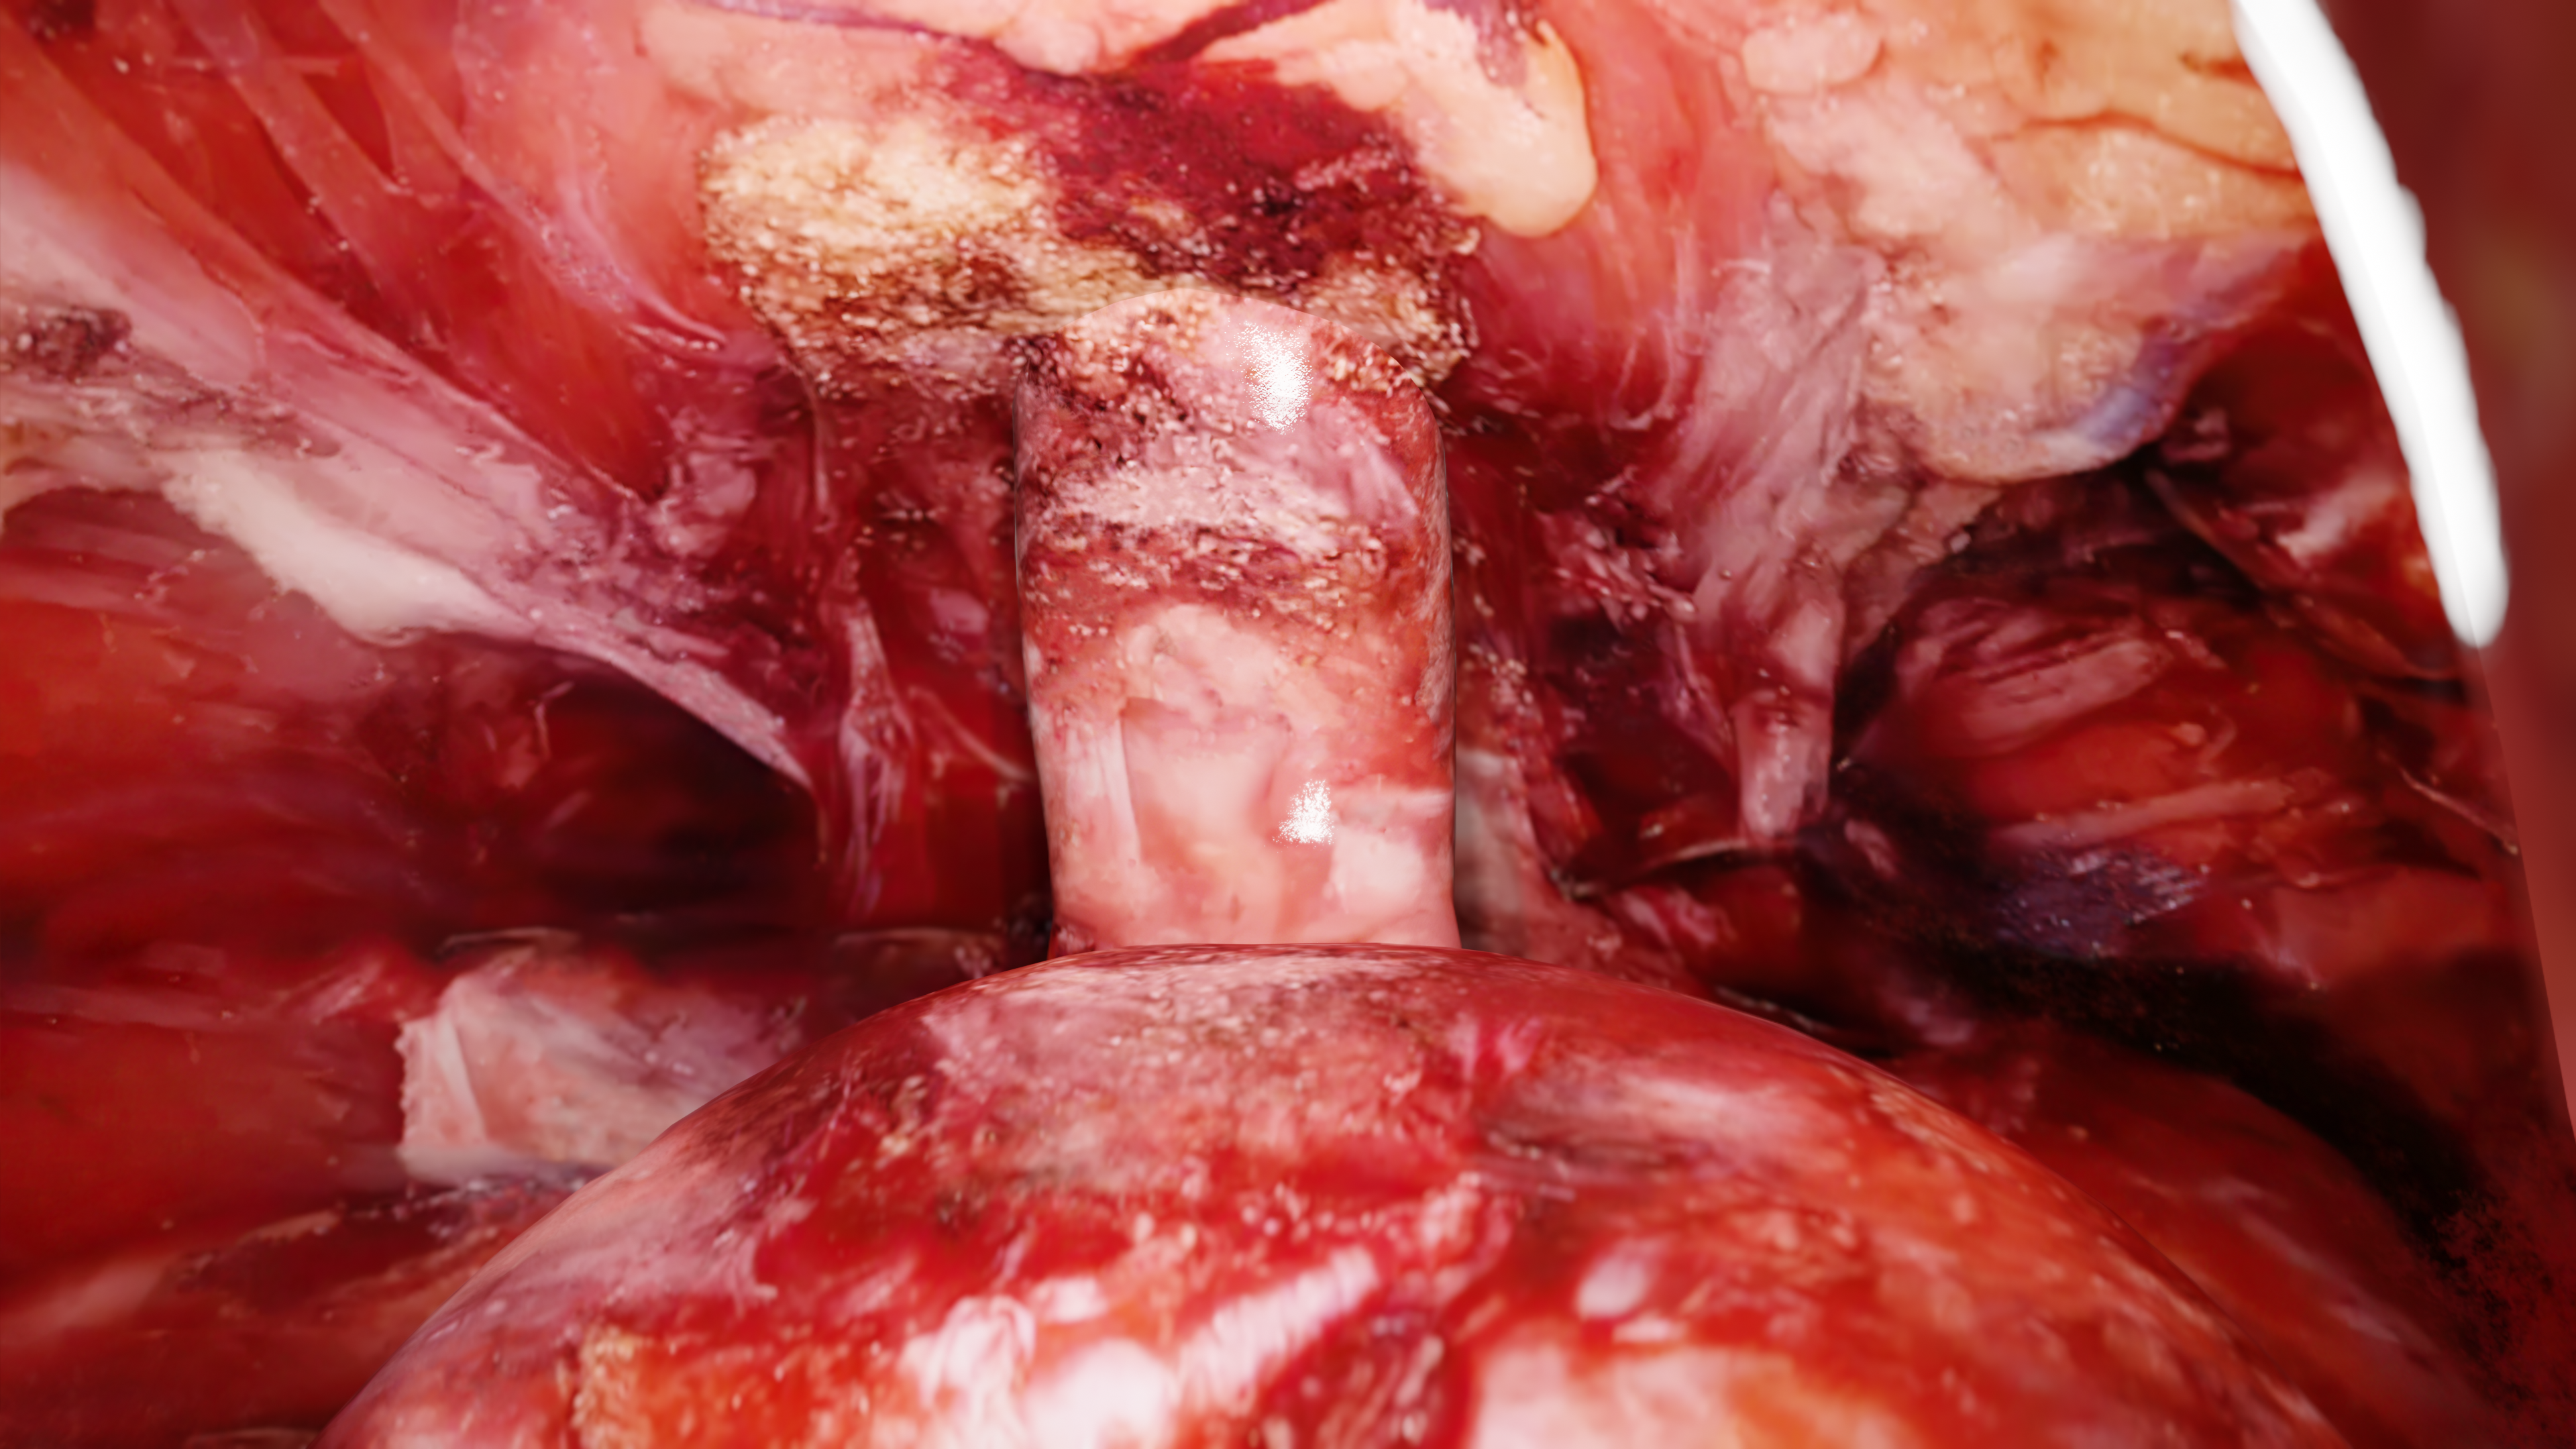
\includegraphics[width=1.0\textwidth,frame]{models/pbr_scene}
  \caption{The scene visualized using physically-based rendering}
  \label{fig:pbr_scene}
\end{figure}

\begin{figure}
  \centering
  \includegraphics[width=1.0\textwidth,frame]{models/urethra_pbr_wireframe}
  \caption{The volumetric part of the urethra with translucent surrounding meshes}
  \label{fig:urethra_pbr_wireframe}
\end{figure}

\begin{figure}
  \centering
  \includegraphics[width=1.0\textwidth,frame]{models/urethra_pbr_foley}
  \caption{A Foley catheter inserted midway through the (translucent) urethra}
  \label{fig:urethra_pbr_foley}
\end{figure}

\subsection{Texture Models}
We're currently extracting background scene and organ textures from stereoscopic recordings of robotic procedures performed at HMC. Our future plan is to extract volumetric textures as well, to render cuts more realistically.


\subsubsection{Textures from Stereoscopic Videos}\label{sssec:videos}
The textures were extracted from a stereoscopic recording of the procedure that is being simulated, and then pasted on top of the surface models that were generated in the previous step. The end result can be seen below.

\begin{figure}
  \centering%
  \setlength{\fboxsep}{0pt}%
  \setlength{\fboxrule}{0.1pt}%
  \fbox{\includegraphics[width=0.48\linewidth]{models/edges}}
  \hfill%
  \fbox{\includegraphics[width=0.48\linewidth]{models/textures}}
  \caption{---}\label{fig:texture_videos}
\end{figure}

\subsubsection{Procedural Textures}\label{sssec:procedural}
To produce seamless and realistic textures in the simulation, we opted to go for procedurally generated textures. Procedural textures are textures created from a user defined procedure instead of using predefined or existing image textures. This provides flexibility in customizing textures, not being limited by source image resolution and to generate textures for different meshes. Blender, a free and open source 3D creation suite supports creating procedural materials using visual programming. The generated textures can then be baked to static images in the required format for rendering later in OpenGL. By using procedural textures instead of textures from real images, we can reduce the time needed in preparing a model.

UV unwrapping a 3D model to a real image of the model to render the texture avoiding seams can be difficult and time consuming. Textures generated from the procedural materials account for the unwrapping, therefore less time can be spent on adjusting the UV coordinates. Moreover, procedural materials can be easily transferred onto other objects as the textures are generated based on the UV unwrapping that would be done beforehand.

\subsubsection{Real-time Rendering}
Blender comes packaged with the option to real-time render the scene which helps in previewing the generated procedural textures, speeding up the cycle of going back and forth between modifying the procedural material and seeing the result.

\begin{figure}
  \centering%
  \setlength{\fboxsep}{0pt}%
  \setlength{\fboxrule}{0.1pt}%
  \fbox{\includegraphics[width=\linewidth]{models/fat}}\\[2ex]
  \fbox{\includegraphics[width=\linewidth]{models/tissue}}
  \caption{Node editor in Blender.}\label{fig:procedural_textures}
\end{figure}

\subsubsection{Node Editor}
Node editor in blender provides a visual way to program the procedural material. The node editor comes with nodes such as different computer generated noise, image mixing, shaders, vector math nodes each with different customizability fields for achieving desired final result. Pairing this up with real-time rendered view leads to an efficient workflow for customizing and creating required materials. A snapshot is included below.

\begin{figure}
  \centering%
  \setlength{\fboxsep}{0pt}%
  \setlength{\fboxrule}{0.1pt}%
  \fbox{\includegraphics[width=\linewidth,frame]{models/blender}}
  \caption{Node editor in Blender.}\label{fig:blender}
\end{figure}

\subsubsection{Model Import}
The models used in our prototypes are volumetric models with tetrahedral structures stored using an OpenVolumeMesh data structure that can handle arbitrary polytopal meshes. Blender is used for surface meshes and is not meant for volumetric meshes. The goal was to import the volumetric mesh, then generate required textures and to export face to UV coordinates mapping for the mesh. However, converting a volumetric mesh to a surface mesh would cause loss of the faces that forms tetrahedrons except for the surface faces, and that could imply loss of vertices.

Unfortunately, it was hard to find methods to convert an OVM mesh to a surface mesh that could be read by blender. Since both VTK and OVM of a mesh had exact vertex to vertex mapping, importing either of them would be fine. We were able to device of two ways to convert a VTK structure into a surface mesh:

\begin{enumerate}[1.]
  \item Import VTK into ParaView and export as supported surface mesh formats, or
  \item Use the VTK Python library, along with VTKBlender library for importing the VTK directly into blender.
\end{enumerate}

Trying out the first method lead to loss of vertices therefore defeating the possibility of exporting UV coordinates. For the second option, the VTK library provided two ways to convert a VTK structure into a surface mesh. The first method was to use surface filter provided by the VTK library, which produced the surface mesh accurately but unused vertices were removed. The second method was to use a geometry filter provided by the same. The latter provided a surface mesh accurately as well, but with all the vertices intact. This meant we could obtain a relationship between the original VTK or OVM and the surface mesh in blender, hence allowing us to successfully map boundary faces of the volumetric mesh to UV coordinates.

\subsubsection{Texture Export}
Once UV unwrapping was done to the imported object and procedural material applied, the process of generating textures was straight forward. Blender provides a way to bake textures which gets the applied material and the UV unwrapping, and generates an image texture based on them.

The surface mesh generated by VTK and VTKBlender library retained all vertices but only kept the surface faces. Due to this, faces between the volumetric mesh and the surface mesh do not have a one to one mapping. However, we can determine the face in the surface mesh that corresponds the face in the volumetric mesh from the vertices for each face.

The surface mesh along with UV coordinates were exported in OBJ format which contains mapping of vertices for each face, and texture coordinates of each vertex for each face. The OVM structure contains face to half-edge mapping, and half-edges have information about two vertices (from- and to- vertex). We managed to create a Python script which maps OBJ faces to OVM faces and then output a file representing face id in OVM and texture coordinates for each unique vertex. The figure below shows the relationship of an OVM face to its corresponding UV coordinates.

We're currently working on generating solid textures that would allow us to render the newly introduced faces, following a cut, properly and more realistically.

\subsubsection{Solid Textures with Random Noise}
The surfaces of the volumetric meshes were textured appropriately by UV unwrapping an identical surface mesh and then mapping UV coordinates to the corresponding surface triangles in the volumetric mesh.

Two types of surface triangles are generated when a user performs a cut on the volumetric mesh. One is parallel to the cut surface and newly introducted, and the other results from subdividing previous surface triangles. In the latter case, we use barycentric coordinates to interpolate the texture coordinates for the resulting triangle from which it was subdivided.

However, for the newly introduced surface triangles that are parallel to the cut surface, we had to follow a different approach. Since the user can cut anywhere on the volumetric mesh, we would need volumetric textures to be super imposed on the newly generated triangles in 3D space.

For the visual look of the cut surface, we chose to use a 3D perlin noise function with tweaked parameters to visualize the cut. We looked into two approaches for volumetric textures. One approach was to generate an $n \times n \times n$ texture using a 3D noise function and then pass it as a 3D texture with OpenGL's \texttt{TEXTURE3D} interface. The other approach was to dynamically generate them within the shader using the 3D noise function. Generating a high resolution volumetric texture that engulfs the whole mesh is time consuming and results in a large memory footprint. Generating a cube texture of dimensions $1000 \times 1000 \times 1000$ would be equivalent of a thousand $1000 \times 1000$ 2D images with the noise computed for each pixel. The second approach seemed to be the better option as the 3D noise function is used only for the pixels within the newly generated triangles and resulted in better performance.

Regardless of the approach, to have continuous textures between cuts, the UVW coordinates (3D coordinates for 3D textures) must be continuous and consistent. By passing the actual XYZ positions of the vertices as UVW coordinates we can render continuous textures between cut surface triangles. However, during user interactions, the texture would change as the mesh deforms because the positions and UVW are the same. To prevent this from happening we use the initial (rest state) coordinates of the vertices in the mesh as UVW coordinates. This initial rest state mesh vertex positions can be considered as UVW mapping of the mesh. The remaining aspect to cover is for the newly generated vertices. These are interpolated using the nearest initial vertices.

\begin{figure}
  \centering
  \includegraphics[width=0.6\textwidth]{models/solid_textures}
  \caption{Shader-based noise texture on the left and precomputed noise texture on the right}\label{fig:solid_textures}
 \end{figure}

\subsection{Material Models}
We've created basic isotropic material models for the urethra and bladder and are iteratively calibrating their parameters using feedback from the experts that are testing out our prototype. Once they're finalized, we'll encode them into our mesh models.

Volumetric models were generated using the TetWild library, which produces meshes that are suitable for \acr{fem} simulations, by using the surface models as input. The output tetrahedral meshes are rendered below.

\begin{figure}
  \centering%
  \includegraphics[width=0.8\linewidth]{models/tets}
  \caption{---}\label{fig:tetra_meshes}
\end{figure}

We're currently at the last step of tweaking the physical parameters to match with the surgeons' expectations.

\clearpage%

% Hamad Medical Corporation
% Georges Younes

\section{Geometric Algorithms for Continuous Collision Detection}\label{sec:continuous_collision}

\subsection{Collision Detection}\label{ssec:collision_detection}
A key challenge is to develop new collision detection algorithms that can be used to check for contacts between deforming objects. One of the issues is to develop scheme that can handle topology changes that are induced by operations such as cutting and suturing. We have been working new techniques to compute the first time of contact between the models using novel continuous collision detection algorithms. Not only do they check for collisions between different objects (e.g.\ organ and the instruments), but they also perform self-collisions between each organ. We dynamically divide the models into clusters that are guaranteed to be non self-colliding. That way, the problem is reduced to checking for collisions between different clusters. The key issue in computing such clusters is to ensure to minimize the number of such clusters during each step of the simulation. We are currently finishing the first prototype implementation and hope to test its performance on the organ benchmarks. The initial testing is performed on a single core CPU, but later we would parallelize them to many-core GPUs. These collision algorithms would be integrated with the finite-element solvers as part of the robust surgical simulation system.

\begin{figure}
  \centering%
  \includegraphics[width=0.55\linewidth]{collision/workflow}
  \caption{Overview of the new dynamic collision-checking algorithm that can handle models undergoing topology changes in deformable models. }\label{fig:dynamic_collision}
\end{figure}

\hrule%

\subsection{Fast Continuous Collision Processing}\label{ssec:fast_ccd}
We have been developing new algorithms for deformable collision detection using hierarchical representations. These include recomputing a new hierarchy based on the mesh topology, traversing the hierarchy and checking for overlaps, and finally between elementary tests for continuous collision detection between the triangle primitives. The continuous collision checks are performed to compute any overlaps between two discrete instances. In order to deal with the topological changes in the mesh caused by cutting operation, we keep track of the changes in mesh connectivity and the new triangles that are added or deleted between successive frames. Our work exploits the local nature of these mesh connectivity changes and performs selective update of the mesh hierarchy that is governed by these incremental changes. In order to perform the selective updates, we use a novel dynamic clustering scheme. Our clustering scheme quickly decomposes the boundary of the objects into non self-colliding clusters based on the meshconnectivity and topology information. This dynamic clustering strategy is general, efficient and involves no precomputation and exploits the high coherence in the simulation results between successive frames of the mesh. Furthermore, we use a merging algorithm that tends to compute tighter-fitting BVH (bounding volume hierarchy). Such tighter hierarchy reduces the number of false positives during the traversal and ultimately reduces the number of elementary tests between the triangle primitives corresponding to the continuous collision checking results. The cluster hierarchy is used to dynamically compute the new BVH using a lazy approach governed by the mesh topology changes.

We assume that we are given a scene composed of one or more objects. Typically each joint organ used in the surgical simulator represents a separately object and is given as a mesh. Each object is represented as a triangle mesh and may correspond to an open or closed object. We assume that it is possible to perform a local inside/outside classification with respect to each triangle in the mesh and that each triangle normal is pointing outward. During the FEM simulation, the objects may undergo motion or deformations, which can change their topology or generate new vertices and triangles; while the connectivity information may change, we assume that the new set of objects are still represented as triangular meshes with local inside/outside classification. Given two discrete time instances in a simulation, we assume that the vertices of the objects move at a constant velocity during that time interval. If new vertices are generated due to topology changes, the CCD (continuous collision checking) problem is then posed as a problem of defining appropriate mapping between the two discreteinstances. Our goal is to check whether there is any collision, including self-collisions, during that time interval, which we represent as $t \in [0, 1]$. For two triangles, this computation reduces to performing 15 elementary tests corresponding to vertex-face (VF) and edge-edge (EE) pairs. Given a CCD query, we assume that there are no collisions among the primitives at $t = 0$. This assumption can be easily checked by using a discrete collision detection algorithm and using the simple BVH.

The simplest general algorithms for CCD between models undergoing topological changes (due to the cutting operation) are based on computing a BVH of all the objects in the scene. The leaf nodes of the BVH correspond to the triangle primitives and the intermediate nodes correspond to the bounding volumes (e.g.\ k-DOPs). Prior CCD algorithms traverse the BVH and perform the CCD queries between the overlapping primitives. Since the connectivity information in the mesh changes when the topology changes, prior techniques that used connectivity information to reduce the number of elementary tests are not directly applicable. As a result, prior algorithms would need to recompute the BVH for the entire scene using top-down or bottom-up manner, which can become expensive for complex scenes with a lot of objects. In order to speed this CCD computation, we decompose the object boundaries into dynamic clusters. Our approach usesa new dynamic clustering scheme. It generates the clusters in an incremental manner by traversing the triangles on the mesh boundary, and makes no assumptions about topology or connectivity changes. We denote these clusters as leaf clusters, which correspond to the lowest level of clusters (or leaf clusters) in the final cluster hierarchy. Moreover, we ensure that each cluster has no self-collisions among its triangle primitives. As a result, CCD reduces to querying only for inter-cluster collisions.

There are two key issues that arise in terms of computing such leaf clusters. The first issue is that, while we want to decompose the boundary into as few clusters as possible, the problem of computing that minimal number of clusters based on some standard criterion (e.g.\ convexity) tends to be NP-hard. To overcome this issue, we compute these clusters using a greedy strategy that exploits the local connectivity and mesh changes. The second issue is that the clusters must be computed efficiently during each frame, as the object’s topology may change from frame to frame. Our next step is to merge these leaf clusters to generate the intermediate clusters; each of these intermediate clusters is also guaranteed to have no self-collisions. Our algorithm merges variousneighboring leaf clusters, while the merged cluster preserve the no self-collision property. The upper level of the hierarchy are obtained by combining various intermediate clusters in a bottom-up manner. At runtime, we traverse the tree in a top down manner and check such cluster bounding volumes for collisions between them using their bounding boxes.

We have finished a preliminary implementation of this algorithm and tested its correctness on simple benchmarks. In the next six months, we propose to integrate them with the outputs of the FEM simulator that are used to implement the cutting operation.

\hrule%

\subsection{Volume Mesh}\label{ssec:volume_mesh}
We are currently considering cutting human tissue open. When the human tissue is not cut, it is a volume and we can represent it as a watertight mesh and represent the internal materials as a discrete set of elements. When the tissue is cut, what we can do is to extend the surface mesh into the cut and stills make the mesh watertight. Our CD algorithm assumes that the mesh is always watertight. This assumption can be implemented using a remeshing tool.

\subsection{KDOP}\label{ssec:kdop}
In order to make CD faster, we do not directly check collision between every pair of n elements (this is $\mathrm{O}(n^2)$).  Therefore, we first use a simple geometry, e.g.\ a box, to bound a set of fine-detailed tissues and check whether these simple geometry collides, if not we do not need costly fine-detailed CD checks. These fine-detailed geometry cannot be too simple, they should represent the fine-detailed tissues reasonably well, KDOPs does this job better than boxes.

\subsection{Front Tracking}\label{ssec:front_tracking}
Front tracking means that between timesteps, your human tissues does not change alot. So that we do not perform CD checks from scratch at each iteration. Instead, we keep track of what's in collision during last timestep and go from there. This makes things faster.

\subsection{Energy-based Collision Response}\label{ssec:energy_based_response}
This is a method where we allow some degrees of collision to remain at every timestep, i.e.\ we do not guarantee collisions are clearly up between timesteps. Instead, we provide a function that grows larger when you have more and deeper penetrations (collisions). Therefore, you can somewhat minimize collisions by minimizing our function.

\subsection{CCD vs.\ DCD}\label{ssec:ccd_vs_dcd}
These are two modes of CD checks. CCD works in continuous time and check whether the movement between two timesteps will cause collision. If so, resolve these collisions and do it until no collisions are remaining. DCD works in discrete time and check wheter the state of mesh at each time instance will cause collision. It does not guarantee collision-free state but runs much faster.

We've included a sample screenshot of a virtual tool interacting with a virtual sphere below, and a more elaborate animated video of the interaction at \url{https://www.dropbox.com/s/8r84zjortzvh5e8/video.mp4?dl=0}.

\begin{figure}
  \centering%
	\includegraphics[width=\linewidth]{collision/cd}
	\caption{---}\label{fig:cd}
\end{figure}

\hrule%

\subsection{Progress during the last six months}
During the past period, we have updated the collision detector (algorithm and routines) to support various detection queries. These queries are needed at different stages of blade and human tissue interactions, which are part of surgical simulation. When the tip of the blade is moving along a prescribed trajectory, our detector performs continuous collision detection (CCD) to check for collisions between the trajectory of the tip and the mesh faces (trajectory/face detection). At the same time, we also performs continuous collision detection between the body of the blade and the mesh edges (body/edge detection). These two detections are used to update the topology of a mesh stored using half-edge data structure.

Besides collision detection, we have also updated the detector to support dynamic boundary volume hierarchy update after the topology of mesh has changed. This involves keeping track of each addition/deletion of edge/face/vertex in the half-edge mesh. On each modification, we update the bounding volume hierarchy (BVH) to add/delete the corresponding node of the hierarchy and make sure that the hierarchy is of high quality and well-balanced so that further queries can be answered efficiently.

Finally, we have setup some standard test routines to make sure the detector works properly. This is done by using a set of standard mesh cuts and perform parity check between the BVH data structure and the half-edge mesh after each cut. A sample animation video is available at \url{https://www.dropbox.com/s/6m4t7kwle8dp1kt/demo.mp4}.

\subsection{Goals for the next six months}
We want to finish this integration of realtime CCD and FEM. As you can imagine, many non-trivial issues are coming up as we try to integrate these two technologies and still try to get realtime performance. Our next goal is to perform detailed performance analysis and demonstrate the results on complex models. There are very few (or none) systems that have performed such tight integration. However, the best way to demonstrate is to:

\begin{enumerate}[\em i\em)]
  \item Evaluate its performance on complex benchmarks, and
  \item Demonstrate the benefits on realtime surgical simulation scenario.
\end{enumerate}

Ultimately, we want to show the actual benefits to the driving application.

\textcolor{Red}{Include content from PR 4 \path{aim_3_technical.pdf}}

\hrule%

Fast collision detection and processing of the intersection of cutting tools with meshes are key operations in surgical simulation. The primary operation while cutting involves the intersection of the cutting tool trajectory with all volumetric elements of the mesh, not just the edges and faces on the boundary surfaces. As described earlier, these intersections are the starting point of the mesh subdivision operations to produce topological separation in the mesh.

The collisions involved in a cutting event must be continuous collisions where all the intersections along the path of the cutting tool movement should be reported, not just the collisions that happen at the starting and ending time instances. We first transform these continuous collisions into discrete collisions by triangulating the path of the cutting tool movement using triangle strips. After that, we detect all the edge-triangle intersections between the cutting tool path and the volumetric mesh. Note that the triangles involve both surface triangles and internal tetrahedral faces of the volumetric mesh.

Another key geometric processing operation involves the contact between the exposed boundary surface elements of the mesh and a rigid non-cutting surgical tool that can hold or push into the body but only on its exterior surface. Continuous collision detection (CCD) methods are needed to robustly detect these collisions, which of course induce deformations in the volumetric mesh that are computed by the finite element model as described in Aim 2. The collisions involved in a non-cutting event can be detected following a conventional CCD algorithm, which consists of two kinds of events: vertex-triangle intersection and edge-edge intersection.

For both cutting and non-cutting events, we use a unified bounding volume hierarchy (BVH) to perform collision culling, which is essential for the high-performance of a collision detection system. However, most previous works only considered constructing a BVH for a mesh with fixed topology in a precomputation step. Other methods use spatial hashing which can be used for changing topologies but involves more computation than BVH because the spatial hashes of every element have to be updated at every frame.

To combine the merits of these two methods, we use a dynamic BVH data structure. We construct an initial BVH for all the surface as well as internal triangular faces for the volumetric mesh using an existing method, which minimizes the SAH-cost function using a greedy algorithm. When edge or vertex intersection queries are required, we first find faces in BVH and then index into the incident edges and vertices. The choice of only constructing one BVH for faces reduces the computational cost to update the BVH after the vertices move.

\begin{figure}
  \centering%
  \includegraphics[width=0.8\textwidth]{collision/BVH}
  \put(-215,102){(\emph{a})}
  \put(-280,17){$C_1$}
  \put(-238,17){$C_2$}
  \put(-217,59){$C_3$}
  \put(-78,102){(\emph{b})}
  \put(-182,17){$C_1$}
  \put(-141,17){$C_2$}
  \put(-60,17){$C_3$}
  \put(-18,17){$C_4$}
  \vspace{-10px}
  \caption{An illustration of iterative BVH updation. We update the BVH at every timestep by first visiting every node in depth first order, so that when we visit a node for the second time, its children have correct and updated bounding volume. During the second visit of an internal node, it can either has three children (\emph{a}) or four children (\emph{b}) with the next two levels. In the case of (\emph{a}), we check whether letting $C_1,C_3$ be sibling or letting $C_2,C_3$ be sibling will improve SAH cost. If so, we apply the corresponding rotation. In the case of (\emph{b}), we check whether letting $<C_1,C_3>,<C_2,C_4>$ be sibling or letting $<C_1,C_4>,<C_2,C_3>$ be sibling will improve SAH cost. If so, we apply the corresponding rotation. In summary, there are two possible rotations to be considered in both cases.}\label{fig:BVHRotation}
  \vspace{-5pt}
\end{figure}

When a topology change happens, the change can be boiled down to two operations: adding new triangular faces and deleting existing triangular faces. When these operations happen, we update our BVH in a brute force manner without performing any tree balancing operations. Specifically, to add a new face, we first search in the BVH for the existing leaf node that is closest to the face, and then use the leaf node as the sibling of the new face node. To delete a face, we use its sibling as its parent node. However, after several topology changes, the BVH will be ill-balances and reconstructing the tree is too computationally costly for a real-time application. To meet the performance requirement, we choose to greedily and iteratively balance the tree. After every frame of the FEM simulation, mesh vertices will move and BVH must be updated accordingly. This update will visit the entire tree in a depth-first manner. When each non-leaf node is visited in this process, we check whether a left-rotation or a right-rotation in the AVL tree balancing algorithm will help reduce the SAH-cost. If so, the operation is applied to the node, as illustrated in \autoref{fig:BVHRotation}. Note that this modification to the BVH update algorithm does not increase the computational complexity, and the complexity of BVH update is still linear in the number of tree nodes. Finally GPGPU implementations are now available, and Aim 4 is continuing integration efforts into the final prototype.

\clearpage%

% Hamad Medical Corporation
% Georges Younes

% % Hamad Medical Corporation
% Georges Younes

\section{Topological Update Algorithms for Incremental Cutting of 3D Meshes}\label{sec:topological_updates}

One modeling challenge in surgical simulation is the geometric and topological representation of cuts and their effects on an underlying tetrahedral mesh. In this section we describe the data structures and algorithms to address this problem. 

Testing push from github to overleaf.

\subsection{Tetrahedral Subdivision Template}

Cutting a tetrahedral mesh should result in a new tetrahedral mesh retaining topological integrity in addition to exhibiting the cut geometrically. We are interested in the set of subdivisions with the granularity to capture general cut topologies.

To simplify the task we consider simple yet versatile subdivisions that can handle general cuts, alleviating the effort of maintaining multiple subdivisions for every cut type. This approach leads to the 1-to-17 universal subdivision \cite{bielser:gm:2004} that divides a tetrahedron into 17 ones to capture general cut patterns.  We note here that these cuts are limited to at most a single cut per edge, and no more than 2 cuts on the edges of a triangular face. These limitations will be addressed with later in this section.

The universal subdivision suffers however from several flaws (details of which are given in a later section), so other, more specialized, subdivisions are needed and have been developed in this work. We use a mixture of modified universal subdivision and the specialized subdivisions in this work. All of the subdivisions employed use the same \enquote{vertex basis} detailed now.

\textbf{Vertices}\\
There are 32 virtual vertices on the surface of a subdivided tetrahedron (these are not all distinct geometrically). Table \ref{tbl:vertices} below lists all of the these vertices split into 3 categories: vertices of the original tetrahedron, vertices at the middle of edges, vertices at the middle of faces. For the subdivision, an edge is split into 2, requiring 2 vertices in the (topological) middle of the edge. A face is split into 4 or 5 triangles and requires 4 vertices in the (topological) middle of the face.

Middle edge vertex notation: 0x.1 indicates the vertex on the edge 01 closest to 0, 0.x1 that closest to 1. Middle face vertex notation: 012x.. indicates the vertex closest to 0, 012.x. that closest to 1, 012..x that closest to 2. Finally, 012 indicates the vertex in the middle of the face 012 \enquote{independent} of the other vertices on the same face, in this write-up it is called \enquote{center mid-face vertex}, and corresponds to the corner vertex of the inside tetrahedron in the universal subdivision.


\begin{table}[]
\begin{center}
\begin{tabular}{|c|c|c|}
\hline
Main Vertex & Mid Edge Vertex & Mid Face Vertex \\ \hline
0           & 4------0x.1     & 16-----012x..   \\ \hline
1           & 5------0.x1     & 17-----012.x.   \\ \hline
2           & 6------1x.2     & 18-----012..x   \\ \hline
3           & 7------1.x2     & 19-----031x..   \\ \hline
            & 8------2x.0     & 20-----031.x.   \\ \hline
            & 9------2.x0     & 21-----031..x   \\ \hline
            & 10-----0x.3     & 22-----132x..   \\ \hline
            & 11-----0.x3     & 23-----132.x.   \\ \hline
            & 12-----1x.3     & 24-----132..x   \\ \hline
            & 13-----1.x3     & 25-----230x..   \\ \hline
            & 14-----2x.3     & 26-----230.x.   \\ \hline
            & 15-----2.x3     & 27-----230..x   \\ \hline
            &                 & 28-----012      \\ \hline
            &                 & 29-----031      \\ \hline
            &                 & 30-----132      \\ \hline
            &                 & 31-----230      \\ \hline
\end{tabular}
\caption{Vertices in the subdivision template. }
\label{tbl:vertices}
\end{center}
\end{table}




\textbf{Edges}\\
The edges of the original tetrahedron are ordered as follows:
\begin{itemize}
    \item 01
    \item 12
    \item 20
    \item 03
    \item 13
    \item 23
\end{itemize}

When the order of the vertices is respected (01 is different from 10) these are interpreted as halfedges. This order can be extracted from a tetrahedral cell of an OpenVolumeMesh mesh in a few steps, first by getting the cell's vertices in its given order, then collecting all the halfedges from each halfface, then checking each one against the halfedges above and placing them in their proper order again based on the order of the vertices of the cell as given by the mesh datastructure. This gives a certain reference to do operations or keep track of information.

When an intersection is detected on an edge, the geometry of the intersection is registered in a property of the mesh at that edge (geometricIntersections). In the subdivision process this information is used to generate vertices to \enquote{materialize} the subdivision. Since each tetrahedron is treated independently, and as an edge is possibly shared by other tetrahedra in the mesh, the generated vertices are shared via another property through the halfedge. In the table this is noted as 0x.1 to indicate the halfedge 01, and 0.x1 to indicate the halfedge 10 (x indicating the from vertex and . indicating the to vertex). The property is called halfEdgeVertices.

\begin{table}[]
\begin{tabular}{|c|c|}
\hline
Intersected Edge & Vertex Information-Held in \\ \hline
01               & 4-0x.1,                    \\ \hline
12               & 6-1x.2,                    \\ \hline
20               & 8-2x.0,                    \\ \hline
03               & 10-0x.3, 11-0.x3           \\ \hline
13               & 12-1x.3, 13-1.x3           \\ \hline
23               & 14-2x.3, 15-2.x3           \\ \hline
\end{tabular}
\caption{--}
\end{table}


Faces
The faces of the original tetrahedron are ordered as follows:

\begin{itemize}
    \item 012
    \item 031
    \item 132
    \item 230
\end{itemize}


This order is not particularly used. Later we discuss a \enquote{cut induced} order when detecting the cutting tool's \enquote{resting} angle, in which this order can be helpful.
As in the case of edges, intersection information is held in a property of the mesh at the face called insidePoints (referring to inside of the face, excluding edges). This property collect all registered intersections in order to compute an average geometry for the vertex or vertices that are added or need to be added on the face. These vertices are also shared between tetrahedra through a face property faceIntersections.

\begin{table}[]
\begin{tabular}{|c|c|}
\hline
Intersected Face & Information Held for \\ \hline
012              & 16, 17, 18, 28       \\ \hline
031              & 19, 20, 21, 29       \\ \hline
132              & 22, 23, 24, 30       \\ \hline
230              & 25, 26, 27, 31       \\ \hline
\end{tabular}
\caption{--}
\end{table}


\subsection{Types of Subdivision}
In the previous section we presented the topological material with which to build subdivisions of a tetrahedron, namely the structure of vertices that would be involved in the subdivision. We now discuss in more details the types of subdivisions used in their details.

We use two \enquote{classes} of subdivisions, the first is the modified universal subdivision and the second is the crack-free subdivision. Both classes use the virtual vertices on the surface of the tetrahedron to construct the child tetrahedra. An important property of the chosen subdivisions is the preservation of edges and faces that are uncut, that is edges and faces not involved in a cut remain undivided and whole.

The modified universal subdivision is a modified version of the 1-to-17 universal subdivision presented in the '99 paper, it conceptually starts off with full subdivision of the tetrahedron, then merges the tetrahdera that lie on a single undivided edge. This reduces the number of child tetrahedra and as importantly preserves a full connectivity with neighbors sharing uncut edges (see figure \ref{fig:Merged_universal_subdivision}). However, since the merging is applied to all uncut edges, whenever a face has all its edges uncut the face itself will be divided to 3 triangles (instead of 6), this is not desirable since it introduces a discontinuity between the 2 terahedra incident to the face. Therefore, for any cut tetrahedron that presents an uncut face, we use a crack-free subdivision that avoids the problem.

\begin{figure}
  \centering%
  \includegraphics[width=0.85\linewidth]{figures/cutting/Merged_universal.png}
  \caption{---}\label{fig:Merged_universal_subdivision}
\end{figure}

The crack-free subdivision described in the '00 paper (Interactive Simulation of Surgical Cuts) relies on tailored subdivisions for each cut topology. They preserve edges and faces that are uncut, however they introduce the possibility of interpenetrating child tetrahedra. To resolve the issue, geometric checks must be made at runtime and a proper subdivision must be chosen.

\textbf{1 Edge Cut}\\
There are 2 faces that are intact when a single edge of the tetrahedron is cut, and therefore using the modified universal subdivision would leave 2 faces subdivided (needlessly), so we use the crack-free subdivision. This subdivision does not have the issue of interpenetrating child tetrahedra.

\textbf{2 Edges Cut}\\
There are 2 types of 2-edge cut. The first (Type A) is when the cuts are on adjacent edges, that is they share a vertex. The second type (Type B) is when the cuts are not on adjacent edges, they are on edges that are on opposite sides of the tetrahedron.

\textbf{Type A}\\
In this case there is a single face that is uncut, and therefore using the modified universal subdivision is not very well suited. The crack-free subdivision for this cut does not suffer from the interpenetrating child tetrahedra and is therefore suitable for use.

\textbf{Type B}\\
The type B cut is possible to have however is (assumed to be) quite rare. This cut leaves no face uncut on the other hand the crack-free subdivision may present interpenetrating child tetrahedraa, therefore we pick the modified universal subdivision for this case.

\textbf{3 Edges Cut}\\
There are 2 types of 3-edge cut. The first, Type A, is when the 3 cuts are on adjacent edges, and therefore the cut removes the shared vertex, separating the tetrahedra into 2 distinct pieces. The second, Type B, is when the 3 cuts are not adjacent, only one of the cut edges is adjacent to the other two. This cut does not separate the tetrahedron (though may come really close to doing so).

\textbf{Type A}\\
Since all three edges are adjacent, they leave a face uncut, so the modified universal subdivision is not well suited. However, the crack-free subdivision presents the interpenetrating child teterahedra issue. Both subdivisions have issues, but since our priority is to leave untouched edges and faces untouched, we choose the crack-free subdivision, and implement geometry checks in order to pick the proper subdivision. Only a single edge-triangle intersection check is necessary to determine whether the subdivision is valid or not, the edge in question is the one that connects a corner of the tetrahedron to the mid point of its opposite face, while the triangle can be any one of a few faces that get all intersected by the given edge. These triangles are faces of child teterahedra that are independent of the vertices of the edge.

\textbf{Type B}\\
This type cuts all faces and therefore we use the modified universal subdivision since it avoids the geometry checks necessary for the crack-free subdivision.

\textbf{4 Edges Cut}\\
When 4 edges are cut, the tetrahedron is always separated, all faces are cut, and we use the modified universal subdivision to avoid the geometry checks of the crack-free subdivision.

\textbf{Summary of used subdivisions}\\
\begin{table}[]
\begin{tabular}{|l|l|}
\hline
Cut Type     & Subdivision Scheme \\ \hline
1-edge cut   & crack-free         \\ \hline
2-edge cut A & crack-free         \\ \hline
2-edge cut B & modified universal \\ \hline
3-edge cut A & crack-free         \\ \hline
3-edge cut B & modified universal \\ \hline
4-edge cut   & modified universal \\ \hline
\end{tabular}
\caption{--}
\end{table}


\subsection{Types and Composition of Cuts}
From the previous sections we have all the blueprints for subdivisions. In this section we present how the geometry of the cuts are computed based on the tables: using the 1-edge cut and 2-edges cut of type A as base cases, and how we give geometries to the necessary vertices that describe/capture the cut to the tetrahedron. The subdivision comes in to insert child tetrahedra using the new geometries, forming an approximation to the cut tetrahedron.

A tetrahedron may be cut at 0, 1, 2, 3 or 4 edges. To represent a cut configuration each edge is assigned a bit: 0 for uncut, 1 for cut. The ordered sequence of these bits representing the states of the edges is called the bitcode. The respected order of the bitcode is that of the edges given in the earlier section, for example 011001 bitcode represents the cuts at edges 12-20-23 (indicating that the vertex 2 has be split off). When an edge is cut, the virtual vertices involved must be materialized. The tables below describe the exact vertices that need to be materialized, along with some topological information (connectivity, or possible connectivity).

An important aspect of the cutting mechanism is that the information for 1-edge cut and 2-edges cut of type A (1-cut and 2A-cut for short) can be universally used to construct the other types of cuts, in this write-up we call these base cut information or splits. The sharp reader may notice that, for a given bitcode, taking the bitwise OR of the splits produces the corresponding bitcode. This is in general a necessary and sufficient condition for producing the splits of any bitcode into the 1-cut and 2A-cut (not the different between 2A-cut and 2-B cut, type B is produced from from 2 1-cuts on opposing edges, while type A is a base case with 2 edges on a single face).

In summary, the topology of the cut is captured in the bitcode, which is decoded into independent 1-cuts and 2A-cuts that materialize the splitting of the virtual vertices and the subdivision blueprint uses the materialized vertices to insert the child tetrahedron, completing the subdivision of the cut tetrahedron.


\textit{1 Edge cut}
\begin{itemize}
    \item 100000 (01): 4 5
    \item 010000 (12): 6 7
    \item 001000 (20): 8 9
    \item 000100 (03): 10 11
    \item 000010 (13): 12 13
    \item 000001 (23): 14 15
\end{itemize}

\textit{2 Edges cut}\\
\textbf{type A}: the 2 cut edges share a vertex. Two adjacent edges may be cut with or without intersection information on the face they share. In the first case the geometry of the mid face vertices is set using the available information - taking the front weighted average of existing intersections, in the second the geometry is chosen to be a linear interpolation (average) between the edge intersection geometries. In both cases the 4 mid face vertices must be split and assigned to their proper topological sides.

The table below describes the geometric and topological assignments of these vertices. When a face is cut the non-center mid face vertices, of which there are 3, must be split into 1-2. The non-center mid face vertex that is separated from the other 2 is named the loner vertex, while the rest are named group vertices. The center vertex must join either side, giving the topological split cases of '1-3' and '2-2'. Naturally, the '1-3' split is named as such because the center vertex is joined to the group, whereas the '2-2' split is named so because the center vertex joins the loner vertex.

For each bitcode the table indicates the loner vertex and the edge vertices (mid loner) from which its geometry can be derived, similarly the group vertices are listed as well as the edge vertices (mid group) from which their geometry can be derived. The 'summit' column in the table indicates the corner vertex of the tetrahedron that is on the side of the loner relative to the face in question, this helps with quick accessing of geometry checks.

The decision of the '1-3' or '2-2' split is based on the which configuration would yield a none interpenetrating tetrahedra in the subdivision, if one option is valid while the other is not then that option is chosen, if both options are valid, then the one with the best 'curvature' is chosen (the center vertex should go with the convex piece of the split face, the center vertex goes \enquote{against} the curvature of the cut), otherwise the center mid vertex is omitted along with its attached tetrahedron.

Currently this logic is only applied in the case of 4-edges cut with the modified universal subdivision, otherwise the 1-3 split is used as it does not cause any issues with the chosen subdivisions in modified universal non 4-edge cases as the 17th tetrahedron is omitted anyway.


\begin{table}[]
\begin{tabular}{|c|c|c|c|c|c|c|c|}
\hline
bitcode & loner & group  & center & mid loner & mid group & summit & comment \\ \hline
110000  & 17    & 16, 18 & 28     & 5,6       & 4,7       & 1      & 01-12   \\ \hline
101000  & 16    & 18, 17 & 28     & 9,4       & 8,5       & 0      & 01-20   \\ \hline
100100  & 19    & 21, 20 & 29     & 4,10      & 5,11      & 0      & 01-03   \\ \hline
100010  & 21    & 20, 19 & 29     & 12,5      & 13,4      & 1      & 01-13   \\ \hline
011000  & 18    & 17, 16 & 28     & 7,8       & 6,9       & 2      & 12-20   \\ \hline
010010  & 22    & 24, 23 & 30     & 6,12      & 7,13      & 1      & 12-13   \\ \hline
010001  & 24    & 23, 22 & 30     & 14,7      & 15,6      & 2      & 12-23   \\ \hline
001100  & 27    & 26, 25 & 31     & 10,9      & 11,8      & 0      & 20-03   \\ \hline
001001  & 25    & 27, 26 & 31     & 8,14      & 9,15      & 2      & 20-23   \\ \hline
000110  & 20    & 19, 21 & 29     & 11,13     & 10,12     & 3      & 03-13   \\ \hline
000101  & 26    & 25, 27 & 31     & 15,11     & 14,10     & 3      & 03-23   \\ \hline
000011  & 23    & 22, 24 & 30     & 13,15     & 12,14     & 3      & 13-23   \\ \hline
\end{tabular}
\caption{--}
\end{table}
% \caption{Groupings of vertex templates on faces.}







\textbf{type B}: the 2 edges cut do not share a vertex, equivalent to two independent 1-edge cuts, therefore all we need to know is which 1-cut information is required to produce the given bitcode. The table below defines for each bitcode of this type which edges to split open.


\begin{table}[]
\begin{tabular}{|l|l|l|l|}
\hline
bitcode & split 1      & split 2        & comment \\ \hline
100001  & 100000 (4,5) & 000001 (14,15) & 01-23   \\ \hline
010100  & 010000 (6,7) & 000100 (10,11) & 12-03   \\ \hline
001010  & 001000 (9,8) & 000010 (12,13) & 20-13   \\ \hline
\end{tabular}
\caption{--}
\end{table}




\textit{3 Edges cut}\\
\textbf{type A}: the 3 edges cut share a vertex cutting it off from the main tetrahedron. These can be solved by independently applying the single edge split on the three edges that are connected to the vertex, and then applying three 2A-cuts on each involved face, each of which is based on the newly created edge splits. The first table gives, for each bitcode, the edges that need to be split, the second table gives the faces that need to be split. The table of edges is very straightforward as every '1' in the bitcode is translated to an edge to split, the table of faces is a bit more involved since it requires all pairs (in this case) of '1' bitcode splits.

(edge)\\
\begin{table}[]
\begin{tabular}{|l|l|l|l|l|}
\hline
bitcode & split 1        & split 2        & split 3        & comment    \\ \hline
110010  & 100000 (4,5)   & 010000 (6,7)   & 000010 (12,13) & cuts off 2 \\ \hline
101100  & 100000 (4,5)   & 001000 (9,8)   & 000100 (10,11) & cuts off 0 \\ \hline
011001  & 010000 (6,7)   & 001000 (9,8)   & 000001 (14,15) & cuts off 3 \\ \hline
000111  & 000100 (10,11) & 000010 (12,13) & 000001 (14,15) & cuts off 1 \\ \hline
\end{tabular}
\caption{--}
\end{table}
% \caption{Edge table for 3 Edges type A cut showing the cut edge components.}


(face)\\
\begin{table}[]
\begin{tabular}{|l|l|l|l|l|}
\hline
bitcode & face 1 & face 2 & face 3 & comment    \\ \hline
110010  & 110000 & 010010 & 100010 & cuts off 2 \\ \hline
101100  & 101000 & 100100 & 001100 & cuts off 0 \\ \hline
011001  & 011000 & 010001 & 001001 & cuts off 3 \\ \hline
000111  & 000110 & 000101 & 000011 & cuts off 1 \\ \hline
\end{tabular}
\caption{--}
\end{table}
% \caption{Face table for 3 Edges type A cut showing the cut face components.}


\textbf{type B}: the 3 edges cut do not share a vertex, 2 adjacent faces are cut at 2 of their edges. This can be solved rather similarly to type A, by first applying the 1-cut splits, then applying only two 2A-cuts on the involved faces. The tables are constructed similarly to their type A counterpart.

(edge)\\
\begin{table}[]
\begin{tabular}{|l|l|l|l|l|}
\hline
bitcode & split 1 & split 2 & split 3 & comment \\ \hline
110100  & 100000  & 010000  & 000100  &         \\ \hline
110001  & 100000  & 010000  & 000001  &         \\ \hline
101010  & 100000  & 001000  & 000010  &         \\ \hline
101001  & 100000  & 001000  & 000001  &         \\ \hline
100101  & 100000  & 000100  & 000001  &         \\ \hline
100011  & 100000  & 000010  & 000001  &         \\ \hline
011100  & 010000  & 001000  & 000100  &         \\ \hline
011010  & 010000  & 001000  & 000010  &         \\ \hline
010110  & 010000  & 000100  & 000010  &         \\ \hline
010101  & 010000  & 000100  & 000001  &         \\ \hline
001110  & 001000  & 000100  & 000010  &         \\ \hline
001011  & 001000  & 000010  & 000001  &         \\ \hline
\end{tabular}
\caption{--}
\end{table}
% \caption{Edge table for 3 Edges type B cut showing the cut edge components.}

(face)\\
\begin{table}[]
\begin{tabular}{|l|l|l|l|}
\hline
bitcode & face 1 & face 2 & comment \\ \hline
110100  & 110000 & 100100 &         \\ \hline
110001  & 110000 & 010001 &         \\ \hline
101010  & 101000 & 100010 &         \\ \hline
101001  & 101000 & 001001 &         \\ \hline
100101  & 100100 & 000101 &         \\ \hline
100011  & 100010 & 000011 &         \\ \hline
011100  & 011000 & 001100 &         \\ \hline
011010  & 011000 & 010010 &         \\ \hline
010110  & 010010 & 000110 &         \\ \hline
010101  & 010001 & 000101 &         \\ \hline
001110  & 001100 & 000110 &         \\ \hline
001011  & 001001 & 000011 &         \\ \hline
\end{tabular}
\caption{--}
\end{table}
% \caption{Face table for 3 Edges type B cut showing the cut face components.}


Note that the middle tetrahedron is not inserted in this subdivision, for visual fidelity. This results in a 1-to-16 subdivision. The deletion of the 17th tetrahedron is not necessary, however it requires a very involved handcrafting of the conditions for each of the 12 cases.


disallowed cuts: these cuts are not allowed since they cut all three edges of a single face, which is not supposed to happen with a single cut segment. These can happen with a sequence of cut segments that are taken to be a single cut, however to get this bit code from a single such cut is rare since it involves very sharp turns, so if it happens, one could handle it by dividing the sequence into parts and applying the parts in order.


\begin{table}[]
\begin{tabular}{|l|l|}
\hline
bitcode & comment  \\ \hline
111000  & face 012 \\ \hline
100110  & face 031 \\ \hline
010011  & face 132 \\ \hline
001101  & face 230 \\ \hline
\end{tabular}
\caption{--}
\end{table}



\textit{4 Edges cut}\\
These can be solved by applying four 1-cuts then four 2A-cuts, the tables follow their counterparts of the 3-edges cut.

(edge)\\
\begin{table}[h]
\begin{tabular}{|l|l|l|l|l|l|}
\hline
bitcode & split 1 & split 2 & split 3 & split 4 & comment \\ \hline
110101  & 100000  & 010000  & 000100  & 000001  &         \\ \hline
011110  & 010000  & 001000  & 000100  & 000010  &         \\ \hline
101011  & 100000  & 001000  & 000010  & 000001  &         \\ \hline
\end{tabular}
\caption{--}
\end{table}
% \caption{Edge table for 4 Edges cut showing the cut edge components.}



(face)\\
\begin{table}[h]
\begin{tabular}{|l|l|l|l|l|l|}
\hline
bitcode & face 1 & face 2 & face 3 & face 4 & comment \\ \hline
110101  & 110000 & 100100 & 010001 & 000101 &         \\ \hline
011110  & 011000 & 010010 & 001100 & 000110 &         \\ \hline
101011  & 101000 & 100010 & 001001 & 000011 &         \\ \hline
\end{tabular}
\caption{--}
\end{table}
% \caption{Face table for 4 Edges cut showing the cut face components.}




Note that, when 4 edges are cut, the central tetrahedron has $2^4$ possible topological configurations: each of its vertices may be on one or the other of the separated pieces of the original tetrahedron (). There are of course only 2 valid configurations as the tetrahedron must be completely attached to only one of the pieces of the split tetrahedron, in addition to the possibility of just not adding it.

The correct decision requires the steps listed in the 2-edges cut type A, to check for interpenetrating tetrahedra for the different possible configurations and deciding based on the geometry of the cut.

\subsection{Cutting Algorithm}
\subsubsection{Core Cutting}

The core cutting algorithms are encapsulated in the CuttingSystem abstraction. The CuttingSystem defines a clean public interface to the cutting mechanism through primarily two cutting methods: one cut and progressive cut. One cut is used when the full cut geometry is known while progressive cut deals with a continuous cut where the cut geometry is not predefined. These methods have guards to prevent any false starts and to ensure proper termination of the procedure. Figure \ref{fig:Cutting_process_flow} shows the flow for the progressive cut.

Both methods are similar in that they invoke BVH intersection method when given cut geometry in the form of triangles approximating the cut surface and segments describing the movement of certain points of the tool. The BVH intersection computation is fast and global. Unlike Bielser’s approach of local (topological) propagation of the cut, the BVH approach allows cutting disconnected parts of a mesh. \ref{fig:BVH_flow}

The intersection information on the edges and faces is used to determine which cells were affected, and in the case of progressive cut, which cells are active, that is the cells that are pierced by the last position of the cutting tool. The active cells are treated differently as their subdivision is not yet complete in the mesh as a subsequent movement of the tool could cut the cell further and cause an internal topology change, handled by the state machine introduced by Bielser. With the intersections completed the cut can be processed. Subdivision can take place and the resulting changes are reported back to the BVH to update its internal structure, and the physics engine to let it know of new vertices and edges that need to be accounted for.

Processing of the cut distinguishes between finalized and active cells, where finalized cells are affected cells that are not active. Each is treated differently primarily because the resulting changes to the mesh need to be treated differently. BVH deals only with the part of the mesh that is possible to intersect, therefore the changes resulting from active cells should not be reported to it. On the other hand, physics should be aware of the exact state of the mesh topology, therefore everything is reported to it. To keep track of the affected, active, finalized cells as well as their children a CutTetrahedronManager object is used to provide all the management functionalities.\ref{fig:Process_cut_details_flow}

Each cell is treated independently. If there is no topology change to the cell, its geometry (its children’s geometry) is updated. Otherwise, the cell gets a first or a new subdivision once the new vertices are determined and set in the mesh. The subdivision process itself is very involved and another point where this work diverges from Bielser’s. First a modified universal subdivision is introduced that merges cells along uncut edges. This does not eliminate “crack”s in the mesh, however in the select cases where it is used, it ensures that uncut edges are not subdivided. We also use the cut-specific subdivisions. The use cases are shown in the subdivision diagram level 3. This mix of subdivision ensures the fewest the introduction of fewer cells, a major drawback of any subdivision based geometry cutting. \ref{fig:CutTetrahedron_flow} \ref{fig:Subdivision_flow}


\begin{figure}
  \centering%
  \includegraphics[width=0.85\linewidth]{figures/cutting/Process_cut.png}
  \caption{---}\label{fig:Cutting_process_flow}
\end{figure}



\begin{figure}
  \centering%
  \includegraphics[width=0.85\linewidth]{figures/cutting/BVH.png}
  \caption{---}\label{fig:BVH_flow}
\end{figure}


\begin{figure}
  \centering%
  \includegraphics[width=0.85\linewidth]{figures/cutting/Process_cut_details.png}
  \caption{---}\label{fig:Process_cut_details_flow}
\end{figure}


\begin{figure}
  \centering%
  \includegraphics[width=0.85\linewidth]{figures/cutting/cuttetrahedron.png}
  \caption{---}\label{fig:CutTetrahedron_flow}
\end{figure}


\begin{figure}
  \centering%
  \includegraphics[width=0.85\linewidth]{figures/cutting/subdivision.png}
  \caption{---}\label{fig:Subdivision_flow}
\end{figure}


\subsubsection{Enhanced Cutting Operations}

\textbf{Adaptive Cutting}\\

\textbf{Mesh Cleanup and Simplification}\\
Once the cut is processed and the mesh updates are done, a further post-process first cleans the mesh of any flat cells and reduces the number of new cells. The mesh simplification algorithm maintains a good mesh topology without cell inversions, a problem that is usually hard to solve globally, it also maintains the geometry of the cut on the mesh as well as the mesh volume for maximum visual fidelity on all levels.

The algorithm operates by iterating on edge contractions. An edge contraction operation on edge $ij$ removes vertex $j$ and reattaches to $i$ all tetrahedra that were incident to $j$. Edge contraction follows an order based on the priority of vertices. Vertices on the cutting surface are of highest priority and are not removed in order to preserve the shape of the cut. Vertices in the interior of the volume have lowest priority and are removed first to simplify the mesh. Vertices on the boundary are next in the priority and are removed as needed to simplify the model while keeping the original volume intact.

\clearpage

\section{Scalable Methods for Non-linear Real-time Finite Element Simulation}\label{sec:fem_simulation}

\subsection{Incremental Introduction of Cuts and Discontinuities in 3D meshes}\label{ssec:discontinuous_fem}
One modeling challenge in surgical simulation is the geometric and topological representation of cuts and their effects on an underlying tetrahedral mesh. Data structures and algorithms to address this problem are described next.

\subsubsection{Tetrahedral Subdivision Template}

Cutting a tetrahedral mesh should result in a new mesh retaining topological integrity in addition to exhibiting the cut geometrically. In order to capture general cut topologies, a tetrahedral subdivision scheme with the granularity to represent various types of topological cuts is needed. To this end we built a generic 32-vertex tetrahedral template, where arrangements of these vertices can generate the various discontinuities that appear during cutting.

\begin{figure}
	\includegraphics[width=0.6\textwidth]{cutting/vertextable.pdf}
	\includegraphics[width=0.4\textwidth]{cutting/face.pdf}
	\caption{Vertices in the subdivision template. The vertices on face 012 are shown on the right.}
	\label{fig:vertices}
\end{figure}

Figure \ref{fig:vertices} lists the 32 virtual vertices on the surface of the template sudivision tetrahedron. These vertices are distinct only topologically, not geometrically. The table lists these vertices in three categories: vertices of the original tetrahedron, vertices at the middle of edges, and vertices at the middle of faces. For the subdivision, an edge is split into 2, requiring 2 vertices in the (topological) middle of the edge. A face is split into 4 or 5 triangles and requires 4 vertices in the (topological) middle of the face. The notation used in the table is as follows. The mid-edge vertex $i\times .j$ denote the vertex on edge $ij$ closest to $i$. The mid-face $ijk\times ..$ denotes the vertex on face $ijk$ closest to the position denoted by the $\times$. The vertex denoted as $ijk$ is the mid-face vertex on face $ijk$.

Assuming that cuts are limited to a single cut per edge and no more than 2 cuts on the edges of a triangular face, these vertices provide the necessary topology for a tetrahedron to be properly subdivided into 17 children tetrahedra. However these subdivisions may be produce incompatible meshes where an edge or face may be subdivided differently depending on the tetrahedra it is connected to. These incompatible subdivisions produce hanging nodes that complicate the physical simulation. In order to avoid these incompatibilities in the mesh, the generic subdivision is modified to merge the children tetrahedra that lie on a single undivided edge. This reduces the number of child tetrahedra and as importantly preserves a full connectivity with neighbors sharing uncut edges. The resulting subdivision template is shown in \autoref{fig:Merged_universal_subdivision}. In addition, subdivided faces with uncut edges are also merged to avoid face cracks between neighboring tetrahedra.

\begin{figure}
  \centering%
  \includegraphics[width=0.85\linewidth]{figures/cutting/Merged_universal.png}
  \caption{Universal subdivision tetrahedral template with merged children along edges.}\label{fig:Merged_universal_subdivision}
\end{figure}


\subsubsection{Types of Subdivision}

The template above supports the five types of topologically-distinct discontinuous tetrahedral elements that occur during incision. The top portion of \autoref{fig:discontinuous_tetrahedra_fem} shows the 1-edge, 2-edge, and 3-edge cases (involving edges sharing a vertex), while the left two pictures of the bottom portion show the 3-edge and 4-edge cases (involving edges around two different vertices). These elements involve planar cuts inside individual elements. A complete cut with compatibility between neighbors is shown on the right of the bottom row.

\begin{figure}
  \centering%
  \includegraphics[width=0.85\linewidth]{simulation/cut_configurations}
  \caption{Cut configurations}\label{fig:discontinuous_tetrahedra_fem}
\end{figure}


One of the challenges of robust cutting is the case of edges that get cut twice. This occurs when tool paths with extensive curvature take place. This configuration is not directly supported by the subdivision template above, and an adaptive refinement of the mesh is needed. We developed a procedure that automatically refines the mesh when a doubly cut edge is encountered. The refinement divides the tetrahedra incident in this edge in such a way as to be able to apply the regular subdivision on the resulting mesh.  An example of this adaptive cut-aware refinement is shown in \autoref{fig:tet_cuts}.

\begin{figure}
  %\captionsetup[subfigure]{width=0.2\textwidth}
  \centering%
  \subbottom[]{\includegraphics[width=0.19\textwidth]{simulation/tet_cut1}\label{fig:tet_cut1}}
  \hfill%
  \subbottom[]{\includegraphics[width=0.19\textwidth]{simulation/tet_cut2}\label{fig:tet_cut2}}
  \hfill%
  \subbottom[]{\includegraphics[width=0.19\textwidth]{simulation/tet_cut3}\label{fig:tet_cut3}}
  \hfill%
  \subbottom[]{\includegraphics[width=0.19\textwidth]{simulation/tet_cut4}\label{fig:tet_cut4}}
  \hfill%
  \subbottom[]{\includegraphics[width=0.19\textwidth]{simulation/tet_cut5}\label{fig:tet_cut5}}
  \caption{This figure shows 2 tetrahedra (\emph{a}), top and bottom, and a cut that intersects an edge separating the 2 tetrahedra (\emph{b}) curves inside the bottom one (\emph{c}) and exits intersecting the same edge. When the second cut is detected, the mesh is refined as seen in (\emph{d}), and the cut reapplied (\emph{e}).}\label{fig:tet_cuts}
\end{figure}


Finally, the subdivision scheme could result under certain conditions in some flat tetrahedra. A post-process is used to clean the mesh from such anomalies. An example is shown in \autoref{fig:flat_tet}. This post-process, that follows the introduction of an incision, is also used to improve mesh quality by removing tetrahedra with poor shapes and aspect ratios. This mesh simplification algorithm operates by iterating on edge contractions. An edge contraction operation on edge $ij$ removes vertex $j$ and reattaches to $i$ all tetrahedra that were incident to $j$. Edge contraction follows an order based on the priority of vertices. Vertices on the cutting surface path are of highest priority and are not removed in order to preserve the shape of the cut. Vertices in the interior of the volume have lowest priority and are removed first to simplify the mesh. Vertices on the boundary are next in the priority and are removed as needed to simplify the model while keeping the original volume intact.


\begin{figure}
  \centering%
  \includegraphics[width=0.3\textwidth]{simulation/tet_flat1}\label{fig:tet_flat1}
  \hspace{10ex}
  \includegraphics[width=0.3\textwidth]{simulation/tet_flat2}\label{fig:tet_flat2}
  \caption{In this figure, the left mesh (3 tetrahedra) admits a single flat cell shaded in blue, on the right the cluster of affected cells are removed and replaced with an equivalent set (4 tetrahedra) without any flat cells.}\label{fig:flat_tet}
\end{figure}

% In the Figure, the left mesh (3 tetrahedra) admits a single flat cell shaded in blue, on the right the cluster of affected cells are removed and replaced with an equivalent set (4 tetrahedra) without any flat cells.

% This task is now complete and has been tested on a variety of configurations. The system has the ability to handle a variety of cutting scenarios that introduce different topological configurations of the cut tetrahedra. Different parameters allow the system to handle different physical parameters, involving more or less or more prestress in the material, as well as different geometric configurations. The figure below includes illustrations of discontinuities introduced in volumetric tetrahedral meshes.  When cuts are introduced, edges may be cut twice requiring additional adaptive tetrahedral refinements that are handled by the system transparently.

These subdivision methods have the ability to handle in a robust manner a variety of cutting scenarios that introduce different topological configurations of the cut tetrahedra. \autoref{fig:cuts} below includes illustrations of discontinuities introduced in volumetric tetrahedral meshes.  When cuts are introduced, edges may be cut twice requiring additional adaptive tetrahedral refinements that are handled by the system transparently.

\begin{figure}
  \centering%
  \setlength{\fboxsep}{0pt}%
  \setlength{\fboxrule}{0.1pt}%
  \fbox{\includegraphics[width=0.32\linewidth]{simulation/snip0}}
  \hfill%
  \fbox{\includegraphics[width=0.32\linewidth]{simulation/snip1}}
  \hfill%
  \fbox{\includegraphics[width=0.32\linewidth]{simulation/snip2}}
  \caption{---}\label{fig:cuts}
\end{figure}

% ----------------------------------------------------------------------

\subsection{Fast Incremental Solver}\label{ssec:incremental_solver}
% \subsubsection{Incremental Cutting Architecture}

\autoref{fig:cutting_process_flow} shows the overall flow of the progressive cutting procedure. The first step in the procedure is to compute intersections of the tool surface path with the edges and faces of the mesh. A \acr{bvh} data structure is used to allow for fast computations of global intersections allowing disconnected parts of the mesh to be cut as the cutting tool is swept. The intersection information on the edges and faces is used to determine which tetrahedral cells are affected and which are active. Affected cells are those that have been intersected by the tool path and active cells are those pierced by the last position of the cutting tool. The active cells are treated differently than others as their subdivision is not yet complete in the mesh as a subsequent movement of the tool could cut the cell further and cause an internal topology change.  When the intersections are completed, the cut can be processed. Subdivision can then take place and the resulting changes are reported back to the \acr{bvh} to update its internal structure, and to the \acr{fe} physics engine to communicate new and deleted vertices and edges.

\begin{figure}
  \centering%
  \includegraphics[width=0.75\linewidth]{figures/cutting/Process_cut.png}
  \caption{Flow of progressive cutting procedure.}\label{fig:cutting_process_flow}
\end{figure}


% Processing of the cut distinguishes between finalized and active cells, where finalized cells are affected cells that are not active. Each is treated differently primarily because the resulting changes to the mesh need to be treated differently. BVH deals only with the part of the mesh that is possible to intersect, therefore the changes resulting from active cells should not be reported to it. On the other hand, physics should be aware of the exact state of the mesh topology, therefore everything is reported to it. To keep track of the affected, active, finalized cells as well as their children a CutTetrahedronManager object is used to provide all the management functionalities.\ref{fig:Process_cut_details_flow}

% Each cell is treated independently. If there is no topology change to the cell, its geometry (its children’s geometry) is updated. Otherwise, the cell gets a first or a new subdivision once the new vertices are determined and set in the mesh. The subdivision process itself is very involved and another point where this work diverges from Bielser’s. First a modified universal subdivision is introduced that merges cells along uncut edges. This does not eliminate “crack”s in the mesh, however in the select cases where it is used, it ensures that uncut edges are not subdivided. We also use the cut-specific subdivisions. The use cases are shown in the subdivision diagram level 3. This mix of subdivision ensures the fewest the introduction of fewer cells, a major drawback of any subdivision based geometry cutting. \ref{fig:CutTetrahedron_flow} \ref{fig:Subdivision_flow}

% The continuous tool path geometry is discretized and represented as a set of triangles approximating the swept cut surface.
Besides the subdivision procedures described in the previous section, the implementation of this incremental cutting architecture requires a number of components to be tightly integrated. First, the continuous tool path geometry \eg \autoref{fig:incremental} needs to be discretized. A triangular surface that approximates the swept path of the moving tool and bounded by the start and end physical positions of the blade is generated and passed to the BVH intersection routines.

\begin{figure}
	\centering%
	\includegraphics[width=0.4\linewidth]{simulation/incremental}
	\caption{Tool path between two successive blade locations.}\label{fig:incremental}
\end{figure}

% At-every-iteration of the simulation, a geometric master model locates the surgical tools, resolves tool-tissue collisions and tissue-tissue collisions, and communicates this information to the finite element model.

Incremental updating of the \acr{bvh} geometry model and \acr{fe} physics models are essential for real-time cutting procedure simulation. The key to incremental cutting is to reuse as much state information as possible from the previous steps and express a new cut state as a minimal and low rank update of the previous one. The figure below shows an example of single tetrahedral being cut incrementally, where the added sub-tetrahedra generate the necessary updates that are passed to the \acr{bvh} and \acr{fe} models. These updates involve information about deleted edges and faces as well as newly added ones. These updates are obviously much smaller in size than the model size, and can therefore be quickly incorporated in the \acr{bvh} and \acr{fe} models, as well as the rendering and \acr{ui} modules of the system. The efficient collection and communication of these changes (also known as topology deltas) are key to the successful integration of the different modules. This was implemented within the cutting system to allow efficient fine-grained communication between the different modules. The system keeps track of all new tetrahedra along with the new and deleted edges and faces per cutting step and communicates the strict necessary information to the other modules.


% We have finished the implementation and testing of the incremental solution strategy which relies on a state machine to change elements from one cut state to another and generate the necessary updates.

\begin{figure}
  \centering%
  \includegraphics[width=0.7\linewidth]{simulation/cut_progression}
  \caption{Progressive cut of tetrahedral element.}\label{fig:discontinuous_tetrahedra_solver}
\end{figure}

Specifically, the fast incremental solver needs a fine-grained communication with a \acr{bvh}, a powerful data structure for tracking geometric objects and accelerating geometric operations such as triangle-segment intersections ubiquitous in the cutting module. An \acr{api} was designed and implemented to allow the cutting module to communicate information to the \acr{bvh}. In particular, the \acr{bvh} \acr{api} allows the cutting module to determine which edges and faces of the mesh have been cut by a particular sweep of a cutting tool, as well as the geometries of these intersections, in logarithmic complexity. The \acr{bvh} module also requires information about all changes in the mesh to be able to update and restructure the hierarchy so it is synchronized with the base mesh to continue supporting intersection queries.


The \acr{fe} model has to also update the solution, including the displacements of the model and the stresses in it, based on the new geometry (cut location) and any contact constraints between tools and tissue. Resolving the finite element system from scratch with every tool movement would preclude real-time operation. Therefore, incremental solution strategies that exploit the nature of the changes to generate the updated displacements and stresses are needed. These changes in the model and contact constraints are formulated as low rank updates of the finite element stiffness matrix and its factorization. As with \acr{bvh}, the key to fast incremental solution is the efficient two-way fine-grained communication between the finite element system and the collision detection and intersection computation system which incorporates bounding volume hierarchy of the geometric representation. The geometric computation system returns intersection information that is used to build incrementally a set of constraints and/or a set of cuts in the volumetric mesh, as well as \enquote{topology deltas} indicating which elements have been removed and which new elements were added. This incremental communication allows fast updates to the factorization of the finite element stiffness system matrix
 and the resulting solution.

Furthermore, cutting the mesh produces modifications and this information must be communicated with the other modules of the system.
For example, the \acr{ui} requires the new surface triangles that are created as the mesh opens up after the cut in order to render the new shape of the mesh.

The result is a complete system controllable through a \acr{ui} that can cut open a volumetric mesh in real time. Cuts can have sharp curvatures---sharper than those that are resolved by the geometric mesh; cuts are incremental: they can completely separate the \acr{3d} mesh or only partially open it; cuts can also intersect each other. We believe these capabilities surpass the state of the art in this area and our early presentations of the system at international conferences have been very well received, with leading groups from around the world requesting access to the system. Below is a screenshot from the running system. Sample animation videos are available at \url{https://www.dropbox.com/s/ly53lbgmy1m2aw2/animm-4cuts.avi} and \url{https://www.dropbox.com/s/rjmw8avzb0dkwpm/animm-liver.avi}.

\begin{figure}
	\centering%
	\includegraphics[width=\linewidth,frame]{simulation/endo_cut}
	\caption{Multiple cuts of a cylindrical model}
	\label{fig:endo_cut}
\end{figure}

\autoref{fig:contact} shows a typical cutting scenario that involves a deformation of the soft tissue by a tool followed by a snipping motion in the case of scissors (the transparent triangular surface shows the snipping motion of the blades of the scissors).
\autoref{fig:sphere} shows various geometrically complex cut paths of a solid sphere discretized by tetrahedral elements to demonstrate the general flexibility and reliability of the progressive cutting procedures.
\begin{figure}
  \centering%
  \setlength{\fboxsep}{0pt}%
  \setlength{\fboxrule}{0.1pt}%
  \fbox{\includegraphics[width=0.5\linewidth]{simulation/snip3}}
  \caption{Deforming and snipping a tube}\label{fig:contact}
\end{figure}

\begin{figure}
  \centering%
	\includegraphics[width=0.4\linewidth]{simulation/sphere_1}\hfill%
	\includegraphics[width=0.4\linewidth]{simulation/sphere_2}\\[1.5ex]
	\includegraphics[width=0.4\linewidth]{simulation/sphere_3}\hfill%
	\includegraphics[width=0.4\linewidth]{simulation/sphere_4}\\[1.5ex]
	\includegraphics[width=0.4\linewidth]{simulation/sphere_5}\hfill%
	\includegraphics[width=0.4\linewidth]{simulation/sphere_6}\\
	\caption{Examples of geometrically complex cuts of a spherical mesh}\label{fig:sphere}
\end{figure}


% Timings of the various steps in the process have been performed. The results of the timings identified one bottleneck that could prevent real-time interaction as the constrains set size increases. Optimizations we performed as a result to remove inactive constraints prior to entering the solution loop. This resulted in a much more responsive system with a stable interaction time for the kinds of meshes needed when cutting urethra and models of similar complexity.

% ----------------------------------------------------------------------

\subsection{Non-linear Solver}\label{ssec:nonlinear_solver}
% The nonlinear solver is necessary when large deformations take place. The solution strategy in this case involves an iterative Newton-like scheme that builds on the linear solve. The challenge for the non-linear solution is to control both the number of iterations and the cost of solving the modified linear problem at every iteration. We have started the development of a strategy that performs an approximate solution for the modified problem at every iteration, based on a hierarchical matrix representation of the stiffness matrix which produce algebraic approximations of off-diagonal matrix blocks and can substantially speed up the solution process.

In simulations of cutting procedures, large deformations generally take place necessitating a nonlinear solution strategy that handles the large kinematics of these deformations. \autoref{fig:tube} shows an example of such deformation where a tube under tension is snipped incrementally. Modifications to the underlying tetrahedral model are generated automatically as the tube is sniped around a cross section by a scissor tool (not shown), and the resulting large nonlinear tube deformations are shown.

\begin{figure}
  \centering%
	\includegraphics[width=0.22\linewidth]{simulation/tube_1}\hfill%
	\includegraphics[width=0.22\linewidth]{simulation/tube_2}\hfill%
	\includegraphics[width=0.22\linewidth]{simulation/tube_3}\hfill%
	\includegraphics[width=0.22\linewidth]{simulation/tube_4}\\

  \centering%
	\includegraphics[width=0.2\linewidth]{simulation/tube_5}\hfill%
	\includegraphics[width=0.2\linewidth]{simulation/tube_6}\hfill%
	\includegraphics[width=0.2\linewidth]{simulation/tube_7}\hfill%
	\includegraphics[width=0.2\linewidth]{simulation/tube_8}\\
	\caption{Progressive cut of a tubular shape (mesh, top; and rendered shape, bottom).}\label{fig:tube}
\end{figure}

We handle the nonlinearities using a local-global strategy, and assume the strain energy of the system comes from the edges of the mesh. The local-global strategy reformulates the potential energy of the system as a minimization problem and introduces auxiliary variables corresponding to the rest-length of the elements. This new problem is linear in the positions of the nodes, and non-linear in the newly introduced variable.

By employing block coordinate descent, we can iteratively solve for the spring directions and node positions separately, allowing us to split each iteration into a simple non-linear local problem with a solution in closed form, and a linear problem involving the global stiffness matrix. Furthermore, the linear problem is independent of the system state, allowing us to benefit from pre-factoring or pre-inverting the system matrix.

Although this method converges slower than Newton's method in terms of the number of iterations, it is more work-efficient and the low computational cost of an iteration makes up for the slow convergence.

Consider a system with $m$ nodes and $s$ elements. Let $\mathbf{K}$ be the stiffness matrix of the system, and let $\mathbf{J}$ be the matrix consisting the stiffness weighted incidence vectors of the springs in its columns. The potential energy of the system can be expressed in the following minimization problem:
\begin{equation}
  E(x) = \min_{\|\mathbf{d}_i\| = r_i} \
  \frac{1}{2}\mathbf{x}^\intercal\mathbf{Kx} -
  \mathbf{x}^\intercal\mathbf{Jd}
\end{equation}
where $\mathbf{x}$ represents the node positions, $\mathbf{d}$ the spring directions, and $r_i$ the rest length of the \textit{ith} spring. To model bending resistance for surface elements, a quadratic bending energy model presented in \cite{Bergou06} is used.

$\mathbf{K}$ can be expressed as the sum of rank-one matrices:
\begin{equation}
  \mathbf{K} = \sum_{i = 1}^s k_i\mathbf{A}_i\mathbf{A}_i^\intercal
\end{equation}
where $\mathbf{A}_i \in R^{m}$ are the spring incidence vectors and we make use of this fact to directly update the inverse of $\mathbf{K}$ (or equivalently, its Cholesky factors), allowing for fast interactive cutting.
%-----------------------------------------------------------------------

% In this section, we outline the parallel implementation of the implicit integrator,
% introduce the cutting algorithm, and present a method for augmenting the system
% to introduce physically-based external interaction.

\subsubsection{Parallel Integrator}
The solution framework is described next, and is implemented both for multicore \acr{cpu}s as well as \acr{gpu}s. Each iteration of the integrator for this framework consists of the following steps:
\begin{enumerate}
  \item Compute the element directions $\mathbf{d}$.
  \item Compute $\mathbf{Jd}$.
  \item Solve $\mathbf{Kx} = \mathbf{Jd}$.
  \begin{enumerate}
    \item Sparse Cholesky factorization
    \begin{enumerate}
      \item Permute the right-hand side $\mathbf{P^\intercal Jd}$.
      \item Solve the equation $\mathbf{(P^\intercal KP)(P^\intercal x)} = \mathbf{P^\intercal Jd}$.
      \item Unpermute the solution $\mathbf{PP^\intercal x} = \mathbf{x}$.
    \end{enumerate}
    % \item Dense matrix inverse
    % \begin{enumerate}
    %   \item Compute $\mathbf{x} = \mathbf{K^{-1}Jd}$.
    % \end{enumerate}
  \end{enumerate}

  \item Repeat from step 1.
\end{enumerate}
where $\mathbf{P}$ is the approximate minimum degree permutation of the
Cholesky factorization of $\mathbf{K}$.

Steps 1 and 2 are fairly straight forward to parallelize. In step 1, we launch a kernel where each thread computes the direction of a single spring. This involves normalizing each spring direction and multiplying by the corresponding rest-length. Step 2 is implemented as a level 3 sparse \acr{blas} operation.

Step 3 uses a pre-computed Cholesky factorization of $\mathbf{K}$ to perform a sparse triangular solve. However, due to the inherently serial nature of triangular solvers, this will have to be preceded with an analysis phase to extract as much parallelism as possible \cite{Mayer09}.

Furthermore, the permutation required at every iteration is a potential performance bottleneck, since it is highly memory bound. However, this can easily be avoided by computing all iterations in the permuted space, thus only permuting at the very first and very last iterations.

Another approach for the linear solution is to pre-compute $\mathbf{K^{-1}}$ and solve the system using dense matrix multiplication. Although this is expected to perform extremely well on \acr{gpu}s, it might not be feasible to store the inverse for very large matrices and will not scale well.

\subsubsection{Effects of cuts on the solver}
Cuts in the mesh are incorporated into the model by deleting and adding elements. Suppose we delete $n$ elements, where each element has a rank-one contribution to the system matrix. This cut corresponds to the following low-rank update:
\begin{equation}
  \mathbf{K}:=
  \mathbf{K} - \mathbf{U}\mathbf{U^\intercal}
\end{equation}
where $\mathbf{U} \in R^{m \times n}$ encapsulates the contributions
of all the deleted springs.

Thus, we can directly update the Cholesky factors or the inverse of the
system matrix. For example, using the dense solver approach we can update
$\mathbf{K^{-1}}$ using the Sherman-Morrison identity:
\begin{equation}
  \mathbf{K}^{-1} :=
  \mathbf{K}^{-1} +
  \mathbf{K}^{-1}\mathbf{U}(\mathbf{I} - \mathbf{U^\intercal K}^{-1}\mathbf{U})^{-1}
  \mathbf{U^\intercal K}^{-1}
\end{equation}
% First, we intersect the edges of the mesh with a cutting surface and accumulate
% the intersected edges in a buffer. These edges are then deleted from the mesh.
In the case of the GPU implementation, the ``topological deltas'' are accumulated in an edge buffer and transfered to the \acr{gpu} and a kernel is launched to construct the matrix $\mathbf{U}$. The Sherman-Morrison identity involves dense matrix multiplication and inversion, which have fast parallel implementations.


\subsubsection{Interaction}
A slight modification of the basic solution strategy is needed to allow for user interaction using dynamic constraints. We can constrain any point on the mesh surface using the method of Lagrange multipliers. First, the constrained point $\mathbf{p_i}$ is expressed as a linear combination of one, two or three vertices:
\begin{equation}
\label{eq:lin_comb}
\mathbf{p_i} =
\alpha_{i_1} \mathbf{x_{i_1}} +
\alpha_{i_2} \mathbf{x_{i_2}} +
\alpha_{i_3} \mathbf{x_{i_3}} =
\mathbf{C_{i,:} x},
\end{equation}
where \autoref{eq:lin_comb} can be thought of as a constraint of the original minimization problem. Next, we augment the orignal linear system with these constraints via the following reformulation:
\begin{equation}
    \begin{bmatrix}
        \mathbf{K} & \mathbf{C}^\intercal \\
        \mathbf{C} & \mathbf{0}
    \end{bmatrix}
    \begin{bmatrix}
        \mathbf{x} \\
        \boldsymbol{\lambda}
    \end{bmatrix}
    =
    \begin{bmatrix}
        \mathbf{Jd} \\
        \mathbf{p}
    \end{bmatrix}
\end{equation}
where $\boldsymbol{\lambda}$ corresponds to the Lagrange multipliers of the constrained problem, and $\mathbf{p}$ to the positions of the constrained points. To allowing for dynamic resizing of $\mathbf{C}$ without having to continuously update the linear system, we reduce the system to the following form:
\begin{equation}
  \begin{bmatrix}
    \mathbf{K} & \mathbf{C}^\intercal \\
    \mathbf{0} & -\mathbf{CK^{-1}C^\intercal}
  \end{bmatrix}
  \begin{bmatrix}
    \mathbf{x} \\
    \boldsymbol{\lambda}
  \end{bmatrix}
  =
  \begin{bmatrix}
    \mathbf{Jd} \\
    \mathbf{p} - \mathbf{CK^{-1}Jd}
  \end{bmatrix}
\end{equation}
where $\mathbf{C}$ can now be updated separately from $\mathbf{K}$, at the cost of having to solve for $\boldsymbol{\lambda}$ in a separate step.
% \begin{figure}[ht]
%   \centering
%   \includegraphics[width=0.25\textwidth]{images/shirt_push_no_back.png}
%   \caption{
%     Dynamic constraints allow for physically based interaction without
%     the cost of continuously updating the entire linear system.
%   }
%   \label{fig:shirt-push}
% \end{figure}

%-----------------------------------------------------------------------

\subsubsection{Results}
\begin{figure}
  \centering
  \includegraphics[width=1.0\textwidth]{simulation/performance_plots.png}
  \caption{Performance of different stages of a single iteration of the sparse serial and parallel implementations. From left to right: linear solve, computation of $\mathbf{d}$, computation of $\mathbf{Jd}$.}\label{fig:performance-iteration}
\end{figure}

\autoref{fig:performance-iteration} illustrates the performance of this framework. Each graph shows the execution time of the serial and parallel implementations of an iteration of the sparse integrator on an increasing number of vertices. This performance allows us to execute a large number of iterations in real-time. \autoref{table:dense} shows how the dense integrator significantly outperforms both the serial and parallel sparse implementations for a relatively small mesh. However, the polynomial complexity of the dense representation will not scale.

\begin{table}[ht]
\caption{Performance of the different solvers on small meshes.}
\centering
\begin{tabular}{lrrr}
\toprule
\multicolumn{3}{r}{Execution Time (ms)} \\
\cmidrule(r){2-4}
\textit{m} & Sparse(\acr{cpu}) & Sparse (\acr{gpu}) & Dense (\acr{gpu}) \\
\midrule
% $9$ & $0.002$& $0.320512$ & $0.007328$ \\
$2590$ & $1.575$ & $1.33437$ & $0.202816$ \\
\bottomrule
\end{tabular}
\label{table:dense}
\end{table}

% We have started the development of a refinement of our non-linear solver that has the potential to produce two key advantages:
% \begin{enumerate*}[(1)]
%   \item it allows a straightforward mechanism for trading real-time solution speed and efficiency with solution accuracy.  We have found that when complex maneuvers are performed on a deformable mesh, a reasonably sizeable subset of teteraheda, faces, and edges may be affected. Resolving all these changes to high-accuracy in real time is not possible. Therefore, an elegant solution is to maintain real-time rates of interaction and display, but allow slightly lower fidelity in the rendered deformations.  This lower-fidelity rendering is only transient however. As soon as the complex maneuver that induces large topological changes slows down, the solver \enquote{catches up} and is able to resolve the deformation to the desired higher accuracy;
%   \item it allows a pre-computed factorization of the system matrix to be reused even when a large portion of the model undergoes large rotations requiring non-linear kinematics to be recomputed for a large set of elements. The system stiffness matrix factorization is updated, very efficiently via low rank updates, only when topological changes are introduced by cutting or suturing.  The refined non-linear solution algorithm is effectively an alternating minimization procedure that alternates on updating nodal positions and element deformations/orientations. The element deformations updates are local in nature, providing a substantial algorithmic benefit. The description of this algorithm and its performance in the context of our overall cutting system will be submitted for publication later this summer.
% \end{enumerate*}
%
% We have wrapped up and tested the developments of the non-linear solver algorithm. Our algorithm is particularly designed for real-time interaction as it allows a pre-computed factorization of the system matrix to be reused even when a large portion of the model undergoes large rotations requiring non-linear kinematics to be recomputed for a large set of elements. The alternating minimization procedure used in the solver alternates on updating nodal positions and element deformations/orientations. The element deformations updates are local in nature, providing a substantial algorithmic benefit particularly on \acr{gpu}'s. A \acr{gpu} kernel to compute the local updates in parallel has been developed to be used in tandem with the stiffness matrix factorization, updated as cuts are introduced.
%
% Fine-tuning and calibrations of the parameters of the non-linear solver were also performed.  The  solver iterates on two types of nonlinearities:
% \begin{enumerate*}[(1)]
% \item the \enquote{outer} non-linearity which involves the active set of constrains; the solution algorithm must iterate until this active set is stable; and
% \item non-linearity of the deformations for a given set of active constraints; this is the inner loop of the iteration and does not need to be solved to final accuracy until a stable active constraint set has been identified.
% \end{enumerate*}


% ----------------------------------------------------------------------

\subsection{GPU Acceleration}\label{ssec:gpu_acceleration}

The solution of the underlying large system of algebraic equations is the main time-consuming portion of a finite element simulation, and it is therefore critical to accelerate this step using \acr{gpu} parallel hardware. The sparse factorization described in the previous section suffers from two difficulties on parallel \acr{gpu} hardware. Its memory footprint and the number of FLOPS it requires scale superlineary with problem size because of fill-in, and the triangular sparse solves introduce an inherent serialization in the solution which prevent efficient parallel execution on manycore processors. As a scalable alternative strategy on \acr{gpu}s, we generate the inverse stiffness matrix in a hierarchical matrix representation format requiring only linear memory footprint.  This reduces the solution problem to multiplying this matrix by a force vector, which can be parallelized very effectively.

Hierarchical matrices are space and time efficient representations of dense matrices that exploit the low rank structure of matrix blocks at different levels of granularity. The hierarchically low rank block partitioning produces representations that can be stored and operated on in near-linear complexity instead of the usual polynomial complexity of dense matrices. In the context of real-time simulation, this near-linear growth is key for the simulation of large realistic models. \autoref{fig:gpu_matrix} below show how a hierarchical matrix is partitioned: some blocks (shown in red) are stored as regular dense matrices, while others of differing sizes are stored as low rank blocks.

\begin{figure}
  \centering%
	\includegraphics[width=0.4\linewidth]{simulation/GPU_block}\vspace{2ex}
	\includegraphics[width=0.9\linewidth]{simulation/GPU_zoom}\\
	\caption{Hierarchical matrix representation: dense blocks are shown in red; the rest of the matrix consists of low rank blocks at different level of granularities.}\label{fig:gpu_matrix}
\end{figure}

The challenges in developing efficient data-parallel \acr{gpu} algorithms come primarily from the irregular tree data structures that underlie the hierarchical representations, and the key to performance is to recast the computations on flattened trees in ways that allow batched linear algebra operations to be performed. We developed new \acr{gpu} algorithms in both \acr{sp} and \acr{dp}. Streams are used to overlap various stages of the computation and hide latencies. Sample performance results are shown in \autoref{fig:gpu_performance}. Our hierarchical matrix-vector multiplication
(\acr{hmvm}) \acr{gpu}-accelerated routines involved in the finite element solution can generate solutions in less than \SI{5}{\milli\second} on a problem with 260 K degrees of freedom, and can achieve over \SI{550}{\giga\byte/\second} on the P100 Pascal \acr{gpu}. These results show that the absolute performance of these operations can very effectively leverage the power of \acr{gpu}'s and, perhaps more importantly, that the optimal linear and log-linear growth of these algorithms allow the scaling of our cutting and suturing models beyond what current state of the art systems can do.

\begin{figure}
  \centering%
	\includegraphics[width=\linewidth]{simulation/GPU_performance}
	\caption{GPU performance of hierarchical matrix-vector multiplication.}\label{fig:gpu_performance}
\end{figure}

We also developed additional \acr{gpu}-accelerated operations including low rank update operations, matrix-matrix multiplication performed by sampling the resulting product using an \acr{hara} scheme,  as well as iterative Newton-Schulz matrix inversion operations.  These state-of-the-art algorithms push the boundary of what is possible to do in real time on \acr{gpu}'s at the fundamental algorithmic level. Their integration in the simulation system allows us to scale the simulations to higher resolution and higher fidelity models.

% We have continued the development of \acr{gpu}-accelerated routines for the \acr{hmvm} operations as well as for the low-rank update operations involved in the finite element solution. Our recent publication on this subject was accepted by the prestigious journal ACM Transactions on Mathematical Software,
%
% We have finished the development of algorithms to support the acceleration of the solution computation when running in the presence of \acr{gpu}'s.

% We have also developed routines for the low-rank update operations involved in the finite element solution.
% The system can now build approximate hierarchical matrix representations of inverses of the stiffness matrices and perform low rank update operations on them in their compressed hierarchical form as the cutting operation progresses.

%
% A recent publication documenting various aspects of these developments has been accepted in the flagship SIAM Journal on Scientific Computing. These state-of-the-art algorithms are pushing the boundary of what is possible to do in real time on \acr{gpu}'s, at the fundamental algorithmic level. Their integration in the simulation system is allowing us to scale the simulations to higher resolution and higher fidelity models.

As examples of the high performance of the system, the figure below shows \acr{gpu} timings and scalability results. The left figure shows the time it takes to construct a hierarchical matrix on a representative problem of various sizes on a P100 nVIDIA \acr{gpu}, while the middle figure shows the corresponding performance achieved on these problems. Problems of size 16,000, which are already useful for high resolution surgical models, achieve a 100\,GFLOPS/s performance. Larger models achieve even higher performance, and the growth in runtime is only log-linear in problem size. The last plot shows a computation of the inverse of a stiffness matrix using an iterative Newton-Schulz method on a problem of size 4,000. Second order convergence is observed, and the whole computation is \acr{gpu}-resident.

\begin{figure}
  \centering%
  \includegraphics[trim=180 200 160 300,clip,width=0.32\linewidth]{simulation/plot0.pdf}
  \hfill%
  \includegraphics[trim=180 200 160 300,clip,width=0.32\linewidth]{simulation/plot1.pdf}
  \hfill%
  \includegraphics[trim=180 200 160 300,clip,width=0.32\linewidth]{simulation/plot2.pdf}
  \vspace{-15ex}
  \caption{Scalability of GPU-accelerated hierarchical matrix operations.}\label{fig:plots}
\end{figure}

% ==========
% In addition, a hierarchical matrix representation of the system stiffness that replaces the sparse Cholesky factors of the stiffness was also tested and timed. This representation may be used for the solution involving simple deformation constraints and updated, via low-rank matrix updates, to account for cuts introduced. Hierarchical matrix representation is the primary mechanism for getting the solution strategy to run on \acr{gpu}'s, as the sparse matrix factors cannot efficiently take advantage of the many cores of the \acr{gpu}'s.
% =========

\autoref{fig:Htests} compares the effectiveness of the hierarchical matrix representation with that of the sparse Cholesky factorization implemented on \acr{gpu}s. The time to solution of the hierarchical matrix solution, once the inverse is computed, is shown to be better than that of a forward and backward passes on precomputed Cholesky factors, and the improvement is more significant as the problem size increases. In terms of memory footprint, the hierarchical matrix inverse requires a little more memory than the sparse factors, however the rate of increase of the memory consumption of the hierarchical inverse slows down as the problem size increases and for larger-scale simulations the curves will cross.

\begin{figure}
  \centering%
  \includegraphics[width=0.4\linewidth]{simulation/sparse_vs_hgemv_time.pdf}
  \qquad\qquad%
  \includegraphics[width=0.4\linewidth]{simulation/sparse_vs_hgemv_memory.pdf}
  \caption{Comparison of hierarchical matrix and sparse factorization solutions on \acr{gpu}s.}\label{fig:Htests}
\end{figure}


\subsection{Faster Time Integration Schemes for Simulation}
\begin{figure}[ht]
  \centering
  \includegraphics[width=0.99\textwidth]{simulation/defo.pdf}
  \caption{Our novel time-integration scheme \acr{pbdd} can simulate deformable objects such as a ball or a large object with large timesteps for realtime applications.}\label{fig:pbdd}
\end{figure}

Many widely-used deformable body simulation packages are based on implicit time-stepping schemes. These methods model the deformable body's governing equation as an \acr{ode} and then integrate the \acr{ode} using high-order numerical schemes. These methods can be arbitrarily accurate but require small timestep sizes. One simple strategy to improve the runtime performance is to use a large timestep size. This strategy has proven successful in some applications, such as controlling humanoid robots, where the timestep size used in a controller can be larger than that used in the underlying simulator. A key issue in using a large timestep size is ensuring that the time integrator is still stable. For example, the stable region of a semi-implicit Euler integrator shrinks as the timestep size increases. To time integrate a deformable body under a large timestep size, a simple and widely-used method is to use an unconditionally stable fully implicit Euler integrator. However, in a conventional deformable body's governing dynamics equation, the use of a fully implicit Euler integrator involves a costly $\mathcal{O}(N^3)$ computation of high-order derivatives, where $N$ is the number of vertices in a deformable body.

The solver of linear systems in \acr{fem} is used as a sub-system in the simulator. On top of it, the simulator uses a time integration scheme to predict the next configuration. To this end, we develop a time-integration scheme that is stable under large timesteps, as illustrated in \autoref{fig:pbdd}. As a results, less timesteps are needed leading to higher efficiency.  We present \acr{pbdd}, a novel optimization-based algorithm for deformable body dynamics simulation. Unlike prior method, which represents the velocity as a time derivative and evaluates this derivative analytically, our \acr{pbdd} formulation represents this velocity using finite differences in the Euclidean space. This Euclidean space discretization allows us to represent all the physical variables as functions of positions. As a result, we can integrate the system implicitly without high-order derivatives. In addition, we show that numerical simulation under our \acr{pbdd} framework can be recast as a numerical optimization. Therefore, our time integrator is stable under an arbitrarily large timestep size because a numerical optimizer can ensure that the energy value decreases during each iteration through line-search or trust region limitation. Solving these unconstrained minimization problems requires evaluating the energy gradient and/or Hessian and solving a linear system of size $\leq N$ where $N$ is the number of vertices.

\begin{figure}[ht]
  \centering
  \includegraphics[width=0.99\textwidth]{simulation/COMP_Stability.pdf}
  \put(-320,-12){(\emph{a})}
  \put(-200,-12){(\emph{b})}
  \put(-070,-12){(\emph{c})}
  \subcaptionphantom{\label{fig:swing_sim_a}}\vspace{-2ex}
  \subcaptionphantom{\label{fig:swing_sim_b}}\vspace{-2ex}
  \subcaptionphantom{\label{fig:swing_sim_c}}\vspace{-2ex}
  \vspace{-2ex}
  \caption{(\emph{a}) We plot the total kinetic+potential energy over time during a standard simulation of a 10-link chain that swings downward. Each joint of this chain is a 2-DOF ball joint so that this chain has 20-DOF. Forward Euler integrator for the Newton-Euler equation and semi-implicit Euler integrator are not stable. Being fully implicit, our second-order \acr{pbdd} solver is stable but quickly loses energy. By increasing the order by one, both the second-order Runge-Kutta and our third-order \acr{pbdd} solver preserve energy very well. (\emph{b}) For the more challenging task of a 100-link chain (200-DOF) that swings downward, even the second-order Runge-Kutta method is not stable and we have to use the third-order Runge-Kutta method for better energy preservation. Our second-order \acr{pbdd} solver is stable but quickly loses energy. Our third-order \acr{pbdd} solver preserves energy very well. (\emph{c}) We compare the total computational time for generating a \SI{10}{\second} trajectory of a 10-link chain swinging down using a second-order collocation method for \acr{pbdd} and a semi-implicit Euler integrator for a conventional formulation. \acr{pbdd} is 1.5--2.1 times slower at a small timestep size and up to 4 times faster at a large timestep size, such as \SI{0.05}{\second}. The faster time integration is used for real-time rigid and deformable simulation.}\label{fig:swing_sim}
\end{figure}

We compare the accuracy of time integrators for our \acr{pbdd} formulation and conventional formulation. In \autoref{fig:swing_sim_a}, we plot the total kinetic+potential energy over time during a standard simulation of a 10-link chain (20-DOF) that swings downward. The timestep size is \SI{0.0025}{\second}. We can see that \acr{pbdd} is very stable and continuously loses energy (\autoref{fig:swing_sim_a} purple). In contrast, low-order explicit integrators such as forward Euler and semi-implicit Euler are not stable. For better accuracy, we can increase the order of integration by one, resulting in a much better performance in terms of energy preservation. In \autoref{fig:swing_sim_b}, we redo the experiment for a 100-link chain (200-DOF). This is more challenging and low-order explicit integrators are more unstable. The Runge-Kutta method for the Newton-Euler equation is stable at the third order. Although our second-order \acr{pbdd} solver suffers a fast energy loss, increasing the order by one can significantly improve accuracy.

\clearpage%

% Hamad Medical Corporation
% Georges Younes

\section{System Integration and Demonstration Prototype}\label{sec:system_integration}

\subsection{Console Setup}\label{ssec:console_setup}
We developed software with the following features:
\begin{enumerate}
  \item Able to load and render DICOM MR images, organ models (derived from MR images), and CAD models of surgical robotic instruments (which include stereoscopic camera, EndoWrist instruments, and trocars),
  \item The user can select and manipulate the positions of the trocars with Fulcrum effect simulated at the incision point (\autoref{fig:simulation_setup}), and
  \item Using the software, one can define the starting scenario for patient-specific simulation of a surgical procedure (\autoref{fig:stereoscopic_console}).
\end{enumerate}

\begin{figure}
  \centering%
  \includegraphics[width=1.0\linewidth]{integration/multiple_views_fusion}
  \caption{Simulation setup rendered by software from different viewpoints.}\label{fig:simulation_setup}
\end{figure}

\begin{figure}
  \centering%
  \includegraphics[width=0.6\linewidth]{integration/console_view}
  \caption{View from stereoscopic camera as seen from surgeon’s console.}\label{fig:stereoscopic_console}
\end{figure}

\hrule%

\subsection{Stereoscopic Rendering}\label{ssec:stereo_rendering}

We have implemented true off-axis stereoscopic rendering as shown below where a two tubes are rendered in Red-Cyan Anaglyph 3D.

\begin{figure}
  \centering%
	\frame{\includegraphics[width=0.5\linewidth]{integration/stereoscopic_anaglyph_red_cyan_rendering}}
	\caption{---}\label{fig:stereo}
\end{figure}

\hrule%

\subsection{Cross-Platform Integration}\label{ssec:cross}
We have created a cross-platform pipeline for continuous integration between our different collaborating teams. Our prototype compiles (using CMake) and runs on all three major platforms: Windows (10 Pro), macOS (High Sierra), and GNU/Linux (Ubuntu Bionic Beaver). We're hosting our private source control repository with \href{https://gitlab.com}{GitLab} to streamline the code access and allow us to experiment with different branches, and are currently working on automating our builds if we were to have more collaborators on board or disseminate our product in the future.

\subsection{User Interface}\label{ssec:console}

We're using robust C++11 libraries and frameworks such as GLFW, GLM, CGAL, Boost, and Eigen, and rendering using OpenGL's Core Profile. We've added support for a bimanual interface using a pair of 3Dconnexion Spaceballs, shown in \autoref{fig:spaceball}, and we're also collecting all the various metrics outlined in Aim 5. This'll allow to replay the procedures as they happened too.

\begin{figure}
  \centering%
  \includegraphics[width=0.32\linewidth]{integration/spaceball_iso_right}
  \hfill%
  \includegraphics[width=0.32\linewidth]{integration/spaceball_front}
  \hfill%
  \includegraphics[width=0.32\linewidth]{integration/spaceball_top}
  \caption{Three views of the 3Dconnexion SpaceBall}\label{fig:spaceball}
\end{figure}

\begin{figure}
  \centering%
  \includegraphics[width=\linewidth]{integration/nanogui_sample}
  \caption{NanoGUI widget library example}\label{fig:nanogui}
\end{figure}

We've added support for Head-up Displays (HUD) using NanoGUI widgets. This'll allow us to display user-friendly notifications and queues, and implement the mockups designed in Aim 5. A sample of the what the library is capable of is shown in \autoref{fig:nanogui}.

An interactive animation from our system integrating the outcomes from the various aims is available at \url{https://www.dropbox.com/s/ax9kmdhaeq91puc/scind_gui.mp4}.

\subsection{Haptic Control}\label{ssec:haptic}
We're using the OpenHaptics framework and the 3D System Touch, shown in \autoref{fig:touch}, to render the forces relayed from the finite element method kernel from Aim 2.

\begin{figure}
  \centering%
  \includegraphics[width=0.48\linewidth]{integration/touch_hero_encoders}
  \hfill%
  \includegraphics[width=0.48\linewidth]{integration/touch_hero_dofs}
  \caption{Different encoders and degrees of freedom for 3D Systems Touch}\label{fig:touch}
\end{figure}

\subsection{Stereoscopisc Rendering}\label{ssec:stereo}
\begin{figure}
  \centering%
  \includegraphics[width=0.45\linewidth]{integration/oculus_rift}
  \hfill%
  \includegraphics[width=0.54\linewidth]{integration/oculus_rift_touch}
  \caption{Oculus Rift and Oculus Touch}\label{fig:oculus}
\end{figure}

We've enhanced our stereoscopic rendering techniques to work better with stereo displays and we're working on extending our routines to support Oculus Rift and Touch shown in \autoref{fig:oculus} for a more immersive experience.

\hrule%

\begin{enumerate}
  \item Photo from spider interface PR #
  \item EndoWrist kinematics slides PR 2
\end{enumerate}

\hrule%

\section{Cross-Platform Integration}\label{sec:cross}

We have integrated more libraries into our CMake-based build process. Our whole system is now under one repository with centralized access to all collaborators.

\section{User Interface}\label{sec:console}
To simulate a realistic presentation of a medical surgery for surgeons to train on, we need to have the same graphical interface as the real surgeries. Hence we need to mimic the graphical interface of the surgical robot in our simulation, but with the addition of feedback queues to help trainees understand their actions during the surgery.

Using a C++ graphical library that can be layered on top of our simulation, easy to use and has no extra/separate code or libraries required, and that works on all three major operating systems: Windows, macOS, and GNU/Linux). To achieve this we decided to try out two of the most popular and widely used C++ graphical user interface libraries: NanoGUI and ImGUI.

\subsection{NanoGUI}\label{ssec:nanogui}
We went with NanoGUI first to assess it according to our requirements. NanoGUI is a minimalistic cross-platform widget library written in C++ for OpenGL which already meets two of the requirements. We started with testing it with our basic requirements by adding images, buttons, inputs, and drop-down menus. The widgets additions were fairly simple and looked promising for our goal, but all of the widgets were windowed, as can be seen below.

\begin{figure}
  \centering%
  \includegraphics[width=0.5\linewidth]{integration/nanogui}
  \caption{---}\label{fig:}
\end{figure}

Next we went on to see if we can make the widgets translucent, especially images. We were able to control the images translucency, but when it came to the other widgets we faced our first obstacle as it wasn’t as direct as the images. For the buttons to be translucent, we had to change the theme of NanoGUI which means it takes effect on multiple widgets that share similar components and all the buttons will be translucent, which does conflict with our needs but it was not a huge issue, and we could work around it by overlaying the transparent widget over an image that act as a non transparent background color for the widget.

Now we need to meet our last requirement, removing the window and the title menu as seen in the figure above. There were no options in NanoGUI to remove them directly, so we needed to find a way to achieve that behaviour. We started with trying to make the title menu completely transparent but with no luck, and same goes for the background of the window. After multiple attempts we managed to bring the widget to the front of both the window and title menu, then resize them to the widget dimensions to make it the only thing visible, as can be seen below with one button. This worked for buttons, text, and inputs, but not for drop-down menus and images. For drop-down menus when clicked on, the dropdown does not show because of the size of the window, while for images, when we make them translucent, the window and title menu show, which is a deal breaker as it violates two of the crucial requirements.

\begin{figure}
  \centering%
  \includegraphics[width=0.4\linewidth]{integration/cropped_button}
  \caption{---}\label{fig:}
\end{figure}

In conclusion, given the behaviour of NanoGUI and the requirements it both met and did not meet, and in addition to the complexity of overcoming some constraints, we marked NanoGUI as an unsuitable tool for this project and other future projects.

\subsection{ImGUI}\label{ssec:imgui}
After deciding on NanoGUI not being a good fit, we moved on to our second option ImGUI. ImGUI is a light-weight graphical user interface library for C++ that is fast, portable, renderer agnostic, and self-contained (no external dependencies). So just like NanoGUI, ImGUI is both written in C++ and cross-platform making it easier for us to integrate it with our simulator. We first started testing ImGUI with removing the window and the title menu, and we managed to do that with only two lines of code, which was a big improvement from NanoGUI both in simplicity and functionality, in addition to controlling the resizing and the movability of the window. After it, we added widgets which had a better structure in the form adding them to our GUI, where each widget such as buttons and labels had their own styling properties that can be applied. In addition, we were able to add images, make them translucent and overlay text on top of them as shown below. Given that, ImGUI met all our requirements, this gave us the green light to go ahead and use it for our graphical interface.

\begin{figure}
  \centering%
  \includegraphics[width=\linewidth]{integration/imgui}
  \caption{---}\label{fig:}
\end{figure}

\subsection{Graphical User Interface}\label{ssec:gui}
We started creating our GUI by looking at the GUI of the da Vinci Robot that is used in the surgeries we are working on simulating for surgeons to train on.

Given these images, we started recreating the widgets in sketch to have them in high resolution to look crisp on all sizes of monitors. In addition, we used our own fonts for the text to give an elegant and simple design to the GUI, especially in the feedback dialogs for the trainees, making it easy for them to read and gentle on their eyes.

\begin{figure}
  \centering%
  \setlength{\fboxsep}{0pt}%
  \setlength{\fboxrule}{0.1pt}%
  \fbox{\includegraphics[width=\linewidth]{integration/davinci_snapshot}}\\[1ex]
  \fbox{\includegraphics[width=\linewidth]{integration/interface_basic_scind}}
  \caption{---}\label{fig:}
\end{figure}

Following this we decided to add a popup window that allows the user to specify options and settings of the scene, in addition to adding a file dialog window, that in the future would give the user the ability to add their own scenes or models to the simulation.

\begin{figure}
\centering%
\setlength{\fboxsep}{0pt}%
\setlength{\fboxrule}{0.1pt}%
\fbox{\includegraphics[width=\linewidth]{integration/interface_basic_scind_popup}}
\end{figure}

Finally, we changed the GUI to match the newest da Vinci robot (da Vinci Xi) with the addition of feedback dialogs. The purpose of this is to replicate the feel of real surgeries, so there is a smooth transition when the trainees transition from our simulator to the da Vinci Xi, in addition to giving them feedback on their progress to reinforce learning the right techniques, by giving them a good explanation of why their actions were not ideal in that scenario and the way to correct them.

\begin{center}
  \setlength{\fboxsep}{0pt}%
  \setlength{\fboxrule}{0.1pt}%
  \fbox{\includegraphics[width=\linewidth]{integration/davinci_xi}}
\end{center}

In conclusion, NanoGUI appeared to be less flexible than ImGUI, giving ImGUI the advantage for us to use it in this project and future projects. Furthermore, we managed to recreate the da Vinci robot GUI to have a simulation that resembles the real feel of surgeries as much as possible, at least when it comes to the graphical interface.

\begin{figure}
  \centering%
  \setlength{\fboxsep}{0pt}%
  \setlength{\fboxrule}{0.1pt}%
  \fbox{\includegraphics[width=\linewidth]{integration/interface_scind}}\\[1ex]
  \fbox{\includegraphics[width=\linewidth]{integration/interface_scind_popup}}
  \caption{---}\label{fig:}
\end{figure}

%\section{Haptic Control}\label{sec:haptic}

%\section{Stereoscopic Rendering}\label{sec:stereo}

\section{SOFA}\label{sec:sofa}
We want to create a robotic surgery simulator similar to what we are making but in using the available solutions that exist to have a comparison to evaluate and measure our solution performance to them.

Using SOFA framework as a tool to develop the robotic surgery simulation. SOFA is an efficient framework dedicated to research, prototyping and development of physics-based simulations that is both open source and cross-platform, this gives the ability to use it freely and modify it on the same three platforms we work on. We wanted to use SOFA since it is extensively used in medical simulation and is mature enough for development since it is been around since 2005.

We want to do the following tasks in SOFA:
\begin{enumerate}[1.]
  \item Loading of both surface and volumetric 3D models (VTK, OBJ, STL, and other),
  \item Deformation of 3D models,
  \item Cutting of 3D models, and
  \item Using the omni phantom as a user input interface.
\end{enumerate}

\subsection{Loading 3D models}
We want to be able to load 3D models to apply the other functions we need. Loading both volumetric and surface 3D models in SOFA was fairly straightforward. Next step, was adding textures to these models, and rendering them was a built-in function.

\begin{figure}
  \centering%
  \setlength{\fboxsep}{0pt}%
  \setlength{\fboxrule}{0.1pt}%
  \fbox{\includegraphics[width=0.7\linewidth]{integration/sofa_textures}}
  \caption{---}\label{fig:sofa_textures}
\end{figure}

\subsection{Deformation}
Next step was us looking at the physics of the engine, specifically the deformation. SOFA provided multiple types for the model to take, Rigid, Vec3, Vec6. The Vec3 type give us the deformable behaviour we want, which is added to the model in the loading part by changing the template. In addition, we used the rigid body template for the scissors as they need not to deform on impact.

\begin{figure}
  \centering%
  \includegraphics[width=0.35\linewidth]{integration/sofa_endowrist}
  \caption{---}\label{fig:sofa_endowrist}
\end{figure}

\subsection{Cutting}
Now we want to implement the cutting to simulate the dissection in a robotic surgery. To achieve this we had to use a SOFA plugin called SOFA Carving Plugin, which gave us the capability to cut a 3D mesh. The cutting was not as advanced as our cutting algorithm, instead it was doing the more basic and traditional way of cutting, which was simply deleting triangles and tetrahedra. We faced issues regarding the cutting in the scene that SOFA was limiting us to be only cutting one model, instead of multiple models, at the same time. In addition, the cutting tool was also limited to one model.

\begin{figure}
  \centering%
  \includegraphics[width=0.35\linewidth]{integration/sofa_cloth}
  \caption{---}\label{fig:sofa_cloth}
\end{figure}

\subsection{Input Interface}
Finally, we worked on integrating the 3DSystems Touch with our SOFA program using another SOFA plugin. We first started with linking keyboard inputs through Python since SOFA allows the use of Python scripts to interact with its environment. Afterwards, we used a plugin provided by SOFA called Geomagic which is the same company that (used) to make the 3DSystem Touch (Omni Phantom) but it is developed by the SOFA team. The plugin gave us the capability of connecting the Touch to SOFA and moving the models using it.

\begin{figure}
  \centering%
  \includegraphics[width=0.5\linewidth]{integration/sofa_interaction}
  \caption{---}\label{fig:sofa_interaction}
\end{figure}

In conclusion, SOFA turned out to be a great choice for us to go with, given all its functionality, but it still has it is own hurdles which we need to work around.

\section{Scenarios Replay}\label{sec:replay}
Our logging module that was mainly developed for Aim 5 and 6, allows us to record the user's actions and replay them. This can be used to recored multiple scenarios and to monitor a user's progress.


\begin{figure}
  \centering%
  \setlength{\fboxsep}{0pt}%
  \setlength{\fboxrule}{0.1pt}%
  \fbox{\includegraphics[width=0.49\linewidth]{integration/snap0}}\hfill%
  \fbox{\includegraphics[width=0.49\linewidth]{integration/snap1}}\\[1.5ex]%
  \fbox{\includegraphics[width=0.49\linewidth]{integration/snap2}}\hfill%
  \fbox{\includegraphics[width=0.49\linewidth]{integration/snap3}}\\[1.5ex]%
  \fbox{\includegraphics[width=0.49\linewidth]{integration/snap4}}\hfill%
  \fbox{\includegraphics[width=0.49\linewidth]{integration/snap5}}\\[1.5ex]%
  \caption{---}\label{fig:cuts}
\end{figure}

\hrule%

\clearpage%

% Hamad Medical Corporation
% Georges Younes

\section{Clinical Validation and Assessment}
\label{sec:clinical_validation}

\begin{itemize}
  \item RARP Surgical substep PR 1 \path{Document4_RARP_Surgical_Substeps.pdf}
  \item Suturing alignment diagrams PR 2 \path{anastomosis.pdf}
  \item Extract suturing alignment diagrams from aim 6 \path{2012.hsmr.docx.pdf}
\end{itemize}

\hrule%

\subsection{Validation and Assessment}
\label{ssec:validation_assessment}

% \textbf{\textcolor{red}{Add definitions of validities and summative/predictive, \etc. }}

Validation is an iterative assessment process throughout the prototype's development cycle to evaluate it from different perspectives: how it looks, how efficient it is, \etc. We choose to conduct face, content and construct validity to evaluate the simulator's realism, appropriateness as a teaching modality and how good it is to differentiate between novice and expert surgeons, respectively.
Face validity refers to the test conducted to assess the subjective realism of the simulator by different urologists that have expertise in robot-assisted radical prostatectomy (RARP). Content validity refers to test is conducted to assess the simulator’s appropriateness as a teaching modality. Construct validity refers to the test that measures how good is the simulator to differentiate between different skills,by collecting various parameters and checking the difference between them when it comes to novice or expert surgeon, for example.
We have developed a validation protocol to be performed after one or few set of features upon the release of a new prototype version. Features shall be assessed by a set of urologists to incorporate their feedback in the next prototype version.

Before the implementation starts, meetings were held with urologists to explain the exact clinical steps, know the parameters to be evaluated by the simulator and how to quantify subjects' performance.

The following points came up during the initial discussion with the surgeons for validation and assessment of a surgical simulator:

\subsubsection{Face Validity}
\label{sssec:face_validity}
\begin{itemize}
  \item Is Face validity dependent on hardware interface irrespective of the software simulation? If yes, as we will be using Mimic frame or Mantis Duo for interface, will the face validity be same as the studies published previously?
  \item Will the result be biased if the clinician providing input during the development phase is also included in evaluation?
  \item Some suggested sample subjective questionnaire to be recorded on Likert scale:
  \begin{itemize}
    \item The interface (hand-foot controllers/visualization interface) provided on the simulator is effective for working in the simulated environment?
    \item The device is sufficient accurate representation of the real robotic system?
  \end{itemize}
\end{itemize}


\subsubsection{Content Validity}
\label{sssec:content_validity}
\begin{itemize}
  \item The subjective study will give a single value for content validity questions. Would it be sufficient?
  \item Will the result be biased if the clinician providing input during the development phase is also included in evaluation?
  \item Sample Subjective Questionnaire to be recorded on likert scale
  \begin{itemize}
    \item The 3D graphical exercises in the simulator are effective for teaching robotic skills
    \item The scoring system effectively communicates my performance on the exercise
    \item The scoring system effectively guides me to improve performance on the simulator
  \end{itemize}
\end{itemize}

\subsubsection{Construct Validity}
\label{sssec:construct_validity}
\begin{itemize}
  \item Some sample objective data metric to be measured by system's software itself:
  \begin{itemize}
    \item Overall score (points) \eg resulting composite metric (total point score or percentage). Robotic surgeons set a relative value of each measure used in the composite score and depends upon the training need. The resulting composite score places the person in threshold levels (which is again defined by robotic surgeon) to evaluate the outcome of pass/fail/warning.
    \item Number of errors (count) \eg tissue ruptures or suture breaks, number of instrument collision, number of times object is grasped and dropped.
    \item Time to complete (seconds)
    \item Economy of motion (centimeters) \eg quality of resection, location and quality of placed sutures, blood loss, instrument going out of view, tissue damage cause by excessive instrument force or unwanted touching, optimum movement of camera.
  \end{itemize}
\end{itemize}




\hrule%

\subsection{Clinical Steps}
\label{ssec:clinical}
The surgical sub-step of cutting the urethra during \acr{rarp} procedure was selected for generation of simulation scenario. The required surgical-steps during \acr{rarp} procedure includes:
\begin{enumerate*}[\em i\em)]
  \item Dropping the bladder,
  \item dividing the neck of the bladder,
  \item exposing the posterior lateral,
  \item cutting the urethra, and
  \item anastomosis.
\end{enumerate*}

Although the approach in performing the surgery might vary between surgeons, \eg whether they perform a transperitonial or an extraperitonial approach, in this project, we simulate only cutting the urethra, which is constant across different variations in terms of requirements, tools and approach.

Urethra dissection is performed by cutting the urethra close to the apex of the prostate, typically with cold scissors to avoid damaging the nearby nerves and structures. Before urethra cutting, cold cutting scissors are used to dissect around it. Occasionally, the \acr{ppl} is cauterized to block bleeding at the side, otherwise cautery is minimized as much as possible in this process as the monopolar current can spread to almost \SIrange{5}{7}{\milli\metre}, which might damage the nearby nerve bundles. The challenge in arriving at the site of the urethra cutting is in carefully dissecting around it. Around the urethra, there is a large vascular complex (called the Dorsal Venous Complex or Santorini's Plexus) and the \acr{ppl}, which the surgeon carefully approaches. As the surgeon dissects through this area, he will be able to recognize the different tissue qualities (muscles, ligaments, veins) until he reaches the urethra and identify the best approach to tackle the dissection.

In preparation before cutting the urethra, it has to be first isolated from the surrounding tissue. The first rule of isolating the urethra is to not skeletonize it: trying to create a perfectly round tube, which will de-vascularize it and remove all the supporting tissue and will potentially cause tearing during the anastomosis process. A surgeon also has to minimize cautery around the urethra as much as possible, to not damage the surrounding tissues and nerves.

Cutting the urethra is an iterative process of cutting, assessing tissue behaviour, and cutting again. The following are the detailed steps observed from prostatectomy videos and described by interviewed surgeons:
\begin{enumerate}[1.]
  \item Create the initial cut,
  \item Move the tools away,
  \item Assess the cut and the tissue behaviour,
  \item Mentally plan the next cut,
  \item Continue cutting,
  \item Repeat steps 2--5, until Foley's catheter is visible
  \item Retract Foley's catheter, and
  \item Circumferentially repeat steps 2--5, until done.
\end{enumerate}

\textbf{Observing tissue behaviour:} In this step, the surgeon is assessing how the tissue behaves as he proceeds with the cutting. This is due to the different types of layers the urethra is made of. For instance, the muscle layer retracts differently from the mucosa layer.

Through our interviews with surgeons, we also identified a list of risky approaches that some surgeons follow but are not recommended for training surgeons. Ideally, the following scenarios should not be allowed in simulations:
\begin{itemize}[$\star$]
  \item Cauterizing the urethra: the only cautery that should happen around that area is at the puboprostatic ligament, which has vessels that could bleed otherwise with cold cutting.
  \item Large cuts: taking a large step can be risky as a large cut can reach to the rectum and puncture it.
  \item Not using a catheter at the site: having a catheter provides the surgeon with a visual cue of where he reaches around the urethra. Not having a catheter might not be ideal for a novice surgeon.
  \item Stretching the urethra before cutting: this will provide a good length for the surgeon but will risk skeletonizing and traumatizing the tissues around the urethra.
  \item Placing the scissors behind the urethra for a better orientation: also, could run at a risk of reaching the rectum behind the urethra.
\end{itemize}

\subsection{Metrics for Performance Evaluation}
%clinical POV
There are two major metrics to evaluate a proper cut of the urethra during prostatectomy: the location of the cut and the shape of the cut. Before the simulation starts, we provide the user with a tutorial on the ideal cutting scenario like location, shape as shown in the sketch in \autoref{fig:ideal_cut} and in \autoref{fig:multiple_planes}.

\subsubsection{Location of the Cut}
Once the surgeon has reached to the urethra (after going through the different structures towards it), he will see on the pelvic wall the dorsal vein complex, the puboprostatic ligaments on each side, and then he will see a tubular structure and the prostate that has been disconnected from the pelvic wall to a certain degree. The surgeon needs to consider a number of factors when determining the location of the cut, including positive tissue margins, staying clear on the sphincters to maintain continence, and the appropriate length of urethra stump to ensure optimum anastomosis with least tissue tension. Other factors depend on the status, location, and aggressiveness of the cancer: the further away from the apex and the less aggressive the cancer is, the closer to the prostate the cut should be located. The staging of the cancer can be defined based on the biopsies taken before the surgery. In general, the location also depends on a surgeon's own judgment from pre-op biopsy and associated Gleason score and cannot be accurately measured or quantified in centimeters as a general rule.

\begin{figure}
  \centering%
  \includegraphics[width=0.5\textwidth]{validation/cut_1}
  \caption{A sketch of the interface showing the user the intended location of cutting}
  \label{fig:ideal_cut}
\end{figure}

\subsubsection{Shape of the Cut}
An ideal shape of the cut is evaluated by three  metrics as described in following sub-sections.

\paragraph{Cutting in One Plane}
\label{par:metric_1}
This means that the cut should be symmetrical, \ie it is only performed in one plane. The plane should be parallel to the plane of the prostate surface. The simulation software should be able to calculate the cutting plane the surgeon is performing and approximate it to one flat plane parallel to the surface of the prostate for a cut to be correctly performed.
\autoref{fig:prostate_surface_plane} shows the plane of the surface of the prostate. An ideal cut should be performed in a plane parallel to this plane, as shown in \autoref{fig:cutting_location_parallel_to_prostate}. Since the training simulation will display the location of the ideal cut, as shown in \autoref{fig:ideal_cut}, a surgeon using this simulation will have a visual cue of the angle of the plane. \autoref{fig:plane_location_orientation} shows the ideal cutting plane location and orientation with respect to the plane of the prostate surface.

\autoref{fig:cutting_in_multiple_planes} show a visual representation of performing a non-uniform asymmetrical cut and how it maps to multiple planes.

\begin{figure}
  %\captionsetup[subfigure]{width=0.3\textwidth}
  \centering%
  \subbottom[The prostate's surface plane]{\includegraphics[width=0.3\textwidth]{validation/cut_2}
  \label{fig:prostate_surface_plane}}
  \hfill%
  \subbottom[The cutting location should be above the apex of the prostate and in one plane parallel to the prostate's surface plane]{\includegraphics[width=0.3\textwidth]{validation/cut_3}
  \label{fig:cutting_location_parallel_to_prostate}}
  \hfill%
  \subbottom[Cutting the urethra should not be performed in a plane not in parallel to the prostate]{\includegraphics[width=0.3\textwidth]{validation/cut_4}
  \label{fig:cutting_location_not_parallel_to_prostate}}
  \caption{The ideal location and orientation of the cutting plane}
  \label{fig:plane_location_orientation}
\end{figure}

\begin{figure}
%\captionsetup[subfigure]{width=0.45\textwidth}
  \centering%
  \subbottom[An example of a non-uniform1 cut performed in multiple planes]{
    \includegraphics[width=0.45\textwidth]{validation/cut_5}
    \label{fig:asymmetrical_cut}
  }
  \hfill%
  \subbottom[Cutting the urethra should not be performed in multiple planes]{
    \includegraphics[width=0.45\textwidth]{validation/cut_6}
    \label{fig:multiple_planes}
  }
  \caption{Cutting in multiple planes}
  \label{fig:cutting_in_multiple_planes}
\end{figure}

\paragraph{One Initial Opening}
\label{par:metric_2}
As a good practice for a clean cut, the surgeon should should perform the task starting from only one initial cut in the urethra and should not create multiple initial cuts.

\paragraph{Cut in Small Steps}
\label{par:metric_3}
Another good practice for a clean cut is cutting only a few millimeters at a time. The minimum and maximum size of a single cutting step is to be defined empirically through test runs and evaluations with surgeons during the formative validity tests.

\hrule%

\subsection{Evaluation Metrics}
\label{ssec:evaluation_metrics}

% \begin{figure}
%   \centering%
% 	\includegraphics[width=0.13\linewidth]{validation/anastomosis_blockage_1}\hspace{2ex}
% 	\includegraphics[width=0.13\linewidth]{validation/anastomosis_blockage_2}\hspace{2ex}
% 	\includegraphics[width=0.13\linewidth]{validation/anastomosis_blockage_3}\hspace{2ex}
% 	\includegraphics[width=0.13\linewidth]{validation/anastomosis_blockage_4}\hspace{2ex}
% 	\includegraphics[width=0.13\linewidth]{validation/anastomosis_blockage_5}
%   \caption{Examples of anastomosis blockage configurations}
%   \label{fig:anastomosis_leakage}
% \end{figure}

In order to evaluate the surgeons performance while using the simulator, several parameters need to be recorded during simulation time. These parameters are based on the aforementioned performance evaluation metrics:

\begin{enumerate}[start=1,label={Para \#\arabic*, }]
	\item \textbf{Plane of the cut:} Cutting in one symmetrical plane: The simulation software shows the user the ideal cutting plane to guide novice user. An option of hiding the ideal plane is also available for more experienced users.

	\item \textbf{Size of the cut:} small snips at a time. The size of a good cut is currently calculated by the surface area that has been separated.  If the surface area is above a certain threshold that has been empirically identified, it is considered a large cut. If it is below, it is considered a good cut. Having big snips may risk in injuring different layers that should not be cut like nerves. [] shows an illustation of big and small cuts on the simulator.

	\item \textbf{Topological cut:} The surgeon should perform the task starting from only one initial cut and continue along the same plane in the urethra and should not create multiple initial cuts. By the end of the simulation, there should exist one continuous cut around the urethra that separates it into two pieces. Whether the surgeon prefers to create one or multiple small cuts initially, they should end up as one eventually. \autoref{fig:ideal_cut} shows an illustration of initial cuts.

	\item \textbf{Rectal wall collisions:} A good practice is to avoid collisions with the surrounding tissues and rectal wall. Injuries in the rectum occur more often during the dissection of the prostatic apex (if not completely mobilized off of the posterior of the prostate). When the rectum stays adherent to the apex, it is at a risk of injury in the process of urethra transecting. \autoref{fig:recWalls} below shows the rectal wall as white-shaded areas.

\begin{figure}
  \centering%
  \subbottom[Side view of rectal wall boarders planes]{
    \includegraphics[width=0.45\textwidth]{figures/validation/rec1.png}
    \label{fig:asymmetrical_cut}
  }
  \hfill%
  \subbottom[Front view of rectal wall boarders planes]{
    \includegraphics[width=0.45\textwidth]{figures/validation/rec2.png}
    \label{fig:multiple_planes}
  }
  \caption{Rectal wall boarders}
  \label{fig:recWalls}
\end{figure}

	\item \textbf{Tools out-of-scene count:} A good practice is to keep surgical tools always visible within the surgical view. Moving the tools out of the scene may result in injuring the patient in a real operation setting. The surgeon shall be able to control the motion of these surgical tools and keep them within his surgical view. \autoref{fig:fov} illustrates the good and back scenarios of this parameter.

  \begin{figure}
    \centering
    \includegraphics[width=.6\textwidth,frame]{figures/validation/fov.JPG}
    \caption{Tools should be always kept within the field of view. Tools out of the scene are dangerous in a real setting}
    \label{fig:fov}
  \end{figure}

	\item \textbf{Time elapsed for task completion:} This parameter will be used to assess the skills acquired by surgeons by using this simulator through their difference in performance parameters throughout trials. This parameter will also be used as an indication to differentiate between different surgeon expertise: a senior surgeon who is used to the console set up perform the task faster than a novice surgical surgeon.
\end{enumerate}

\hrule%

\subsection{Graphical User Interface}
A graphical user interface is needed to communicate the score of the surgeon based on his or her performance in completing the cutting task and to inform the surgeon of ways to improve the performance. In this section, we present the three main screens of this simulator:
\begin{enumerate}[1.]
  \item Pre-simulation: to inform the surgeon of the scoring mechanism
  \item Simulation: to display feedback on the surgeon's performance in real-time
  \item Post-simulation: to provide an overview of the surgeon's performance and the total score
\end{enumerate}

The simulation starts with a total score of 100. The score decreases as the surgeon performs any of the following errors:
\begin{enumerate}[1.]
  \item The surgeon cuts outside the target line and ends up with an asymmetrical cut (\textbf{-10} overall)
  \item The surgeon creates more than one initial cut (\textbf{-10} per initial cut)
  \item The surgeon cuts larger than the accepted threshold per cut (\textbf{-5} per large cut)
  \item The surgeon unnecessarily collides the tool with the tissue (\textbf{-1} per collision)
  \item The surgeon's tool leaves the surgical scene (\textbf{-2} each time)
\end{enumerate}

\subsubsection{Pre-Simulation}
Before the start of the simulation, the subject is taken through a presentation about the simulator in general: the clinical problem, proposed solution, anticipated outcomes, simulator-related instructions, \etc. Then, upon the start of the simulator,a graphical user interface, presented as a mockup in \autoref{fig:pre_training_mockup}, visually presents to the surgeon instructions to correctly perform the cutting task. The first instruction (starting from the top left) is to follow the line displayed over the urethra for the ideal cutting location. The second is related to the metric presented in \autoref{par:metric_1}. The third is related to the metric presented in \autoref{par:metric_2}. The fourth is related to the metric presented in \autoref{par:metric_3}. The fifth and sixth are recommended practices in surgery to avoid collisions with tissues and to keep the tool within the field of view.
\begin{figure}
  \centering%
  \includegraphics[width=1\textwidth]{validation/pre_training}
  \caption{A mockup of the pre-training screen}
  \label{fig:pre_training_mockup}
\end{figure}

\subsubsection{Per-Simulation}
This graphical user interface, presented in all its possible scenarios as multiple mockups in \autoref{fig:training_mockup}, shows the graphical representations of communicating an error to the surgeon. In the default case, the surgeon's simulator screen has little to no information displayed other than the surgical scene and the time elapsed since the start of the cutting task. In case of creating an asymmetrical cut (related to \autoref{par:metric_1}), the deviation is highlighted in red for the surgeon to visualize the cutting error and deviate back to the correct track. In case of creating multiple initial cuts (related to \autoref{par:metric_2}), the location of any other cut made other than the first one is highlighted in red. In all other error cases, a message will be displayed to the surgeon.
When the surgeon hits the rectal wall, the circumference of the simulator screen will turn red, prompting the surgeon to retract his surgical tools. In the case where the surgeon takes his tools out of the scene, a caution sign will appear indicating the exit of surgical tools and prompting the user to return them back within surgical view.
Note that all error visualizations and messages disappear within a few seconds to minimize distractions from the main task and to optimize the focus of the surgeon on cutting.
\begin{figure}
  %\captionsetup[subfigure]{width=0.45\textwidth}
  \centering%
  \subbottom[Default view]{\includegraphics[width=0.45\textwidth]{validation/training_1}}
  \hfill%
  \subbottom[Error: asymmetrical cut]{\includegraphics[width=0.45\textwidth]{validation/training_2}}
  \\
  \subbottom[Error: multiple initial cuts]{\includegraphics[width=0.45\textwidth]{validation/training_3}}
  \hfill%
  \subbottom[Unnecessary collusion with surrounding organs]{\includegraphics[width=0.45\textwidth]{validation/training_4}}
  \caption{A mockup of the training screen and the different possible scenarios}
  \label{fig:training_mockup}
\end{figure}

\subsubsection{Post-Simulation}
This graphical user interface, displayed upon the completion of the cutting task, displays to the surgeon the total score as well as a breakdown of the errors performed during the task. An example is presented in the mockup in \autoref{fig:post_training_mockup}. In this example, the surgeon has scored a total of 76\%, with an asymmetrical cut, two instances of large cuts, and four unnecessary collisions between the tool and the tissue. The interface also displays to the user options to repeat the task or exit the simulation.
\begin{figure}
  \centering%
  \includegraphics[width=.7\textwidth]{validation/post_training}
  \caption{A mockup of an example of results screen}
  \label{fig:post_training_mockup}
\end{figure}

\subsection{Evaluation Protocol}

The validity tests we performed during the development stage of the project are carried in a form of a formative usability study. A formative usability study is an iterative process of multiple usability testing approaches to evaluate the system being developed and assess the integration of features to ensure detecting and eliminating usability issues early before the final design is produced.

Formative evaluation focuses on qualitative results collected from a variety of evaluators, including the design and development team, experts in the field, and target users. In the case of our simulation interface, participants in formative evaluations include the research team, expert surgeons, surgery training professionals, medical doctors with a background in prostatectomy, and surgeons-in-training. These methods are tailored to focus on the face, content and construct parameters of the simulator.

The data collected from the described formative usability testing methods is primarily qualitative.  This data can be later categorized into areas of improvement and used to enhance the simulator for running the next iterations of formative evaluation tests. This qualitative data describes the state of each of the heuristics for face, content and construct validity and list usability issues to be resolved and areas of improvement.

We conducted two formative evaluation tests: heuristics evaluation and think-aloud evaluation.

Once a significant set of features are added to the prototype, a proper usability evaluation with both qualitative and quantitative data is performed. Qualitative data becomes crucial to objectively quantify the surgeon performance rather than getting subjective qualitative feedback.


Towards the end of the project, summative usability study is performed. Summative study is quantitative evaluation with representative users where they are required to perform usability studies, collect their performance measures and perform statistical analysis. This test is mainly done before the end of the project to compare it with initial requirements and test its overall usability.

\subsubsection{Heuristics Evaluation}
Heuristics evaluation is a formative evaluation method for finding the highest number of usability issues before the final design is produced. A list of heuristics is generated and tested through using the system of interest by a group of evaluators.

\paragraph{Study Participants}
For formative study, the participants (or evaluators) are not the target users, but usability experts and domain experts. A diverse group of evaluators ensures finding different types of and more usability issues. In the case of this project, this includes expert surgeons (whom this project is not targeted for, but can provide insights on the usability of the interface), the research team, and medical doctors with a background in prostatectomy.

In summative study, targeted users (end users) are asked to perform these evaluations, while focusing on quantitative analysis. Targeted users for this project are medical doctors who are training on how to use the DaVinci console.

\paragraph{Study Structure}
In heuristics evaluation, evaluators participate in two sessions: individual and group. In the individual session, the evaluator performs the cutting task and discusses a number of heuristics with the test moderator or the main usability researcher. In the group session, evaluators discuss their individual findings and propose solutions to these problems. The following is the detailed structure of each session.

\subparagraph{Individual Evaluation Session} A session for where the evaluator individually completes and discusses the cutting task with the test moderator.
\begin{enumerate}[1.]
  \item Introduction (standardized with all evaluators):
  \begin{enumerate}[\em a\em)]
  \item Provide an overview of the project and the heuristics evaluation method,
  \item Describe the current state and capabilities of the system,
  \item Describe (and demo, if necessary) the cutting task.
  \end{enumerate}
  \item Allow the evaluator to freely use and explore the interface,
  \item Guide the evaluator through the task, while discussing the heuristics,
  \item Record the usability problems encountered or reported by the evaluator.
\end{enumerate}

\subparagraph{Group Debriefing Session}
After individually testing with all the evaluators, organize a group meeting, list all the problems encountered with all evaluators, and discuss possible solutions.

\paragraph{Cutting Task Heuristics}
\begin{enumerate}[1.]
  \item Face Validity:
	\begin{enumerate}[\em a\em)]
	  \item The cutting mechanism represents a real world cutting task in a prostatectomy surgery
	  \item The device is a sufficiently accurate representation of a real robotic system
	  \item The hand controllers are effective for working in the simulated environment
	  \item The user interface is efficient and minimalistic
	\end{enumerate}

  \item Content Validity:
	\begin{enumerate}[\em a\em)]
	  \item The cutting task is effective for teaching the cutting skill for our target users
	  \item The scoring system effectively communicates the user's performance on the cutting exercise
	  \item The scoring system effectively guides the user to improve the performance on the simulator
	  \item The scoring system is effectively communicated to the user and messages are presented in plain language
	  \item Learning the system is feasible by first-time users with minimal supervision/training
	\end{enumerate}

  \item Construct Validity:
	\begin{enumerate}[\em a\em)]
	  \item The system is able to distinguish between an experienced and a novice user based on errors
	  \begin{enumerate}[\em i\em)]
	    \item Number of times the cutting tool damages the tissue with unnecessary touches/cuts
	    \item Number of times the cutting tool goes outside the defined boundary
	  \end{enumerate}
	  \item The system is able to distinguish between an experienced and a novice user based on shape of cut
	  \begin{enumerate}[\em i\em)]
		  \item An interpolated plane of the overall cut (with a threshold for error tolerance)
		  \item The number of centimeters per small cut
		  \item The number of initial cuts
	  \end{enumerate}
	  \item The system is able to distinguish between an experienced and a novice user based on general statistics
	  \begin{enumerate}[\em i\em)]
		  \item Time taken to complete the test
	  \end{enumerate}
  \end{enumerate}
\end{enumerate}

\subsubsection{Think-aloud Evaluation}
Contrary to heuristics, the think-aloud method is performed with target users. In this method, the only data collected from the user is their thinking process throughout using the simulation and while completing the cutting task. Also, contrary to heuristics, the test moderator does not interfere or discuss the interface with the participant. Similar to heuristics, task completion is performed individually. This method is performed in three simple steps:

\begin{enumerate}[1.]
  \item Recruit representative subjects (target users)
  \item Ask the subjects to complete the cutting task and describe their mental process as they complete the task
  \item Meanwhile, the test moderator records the session and takes note of the interaction
\end{enumerate}

Following the session, the subjects filled a qualitative evaluation form including Likert-scale questions relating to face and content validity and discussed the interface informally with the team.

\hrule%

Based on the heuristic evaluation protocol, we prepared a questionnaire on a Likert Scale of 1 to 5, with 1 being \enquote{Strongly Disagree} to 5 being \enquote{Strongly Agree,} to validate and assess the simulator for face and content validity. The questions on Likert Scale will assist in assessing:
\begin{enumerate}[\em i\em)]
  \item The subjective realism of the simulator, \ie the face validity, and
  \item Its appropriateness as a teaching modality, \ie the content validity.
\end{enumerate}

The questionnaire was provided to the evaluators after allowing them to freely use and interact with the cutting simulator. While using the cutting simulator, they were engaged in a discussion with the validity test moderator to assess the usability. Information about the participants (\emph{evaluators}) was collected. This enable classification of the feedback based on the experience level and specialization of the evaluator.

Secondly, we have started implementation of the clinical metric for logging user interactions to assess construct validity. We have identified the information, described in Aim 5: Training and Test Scenarios, to be logged during the interaction of the evaluator with simulator. The information will be displayed after the completion of the task, as displayed in the graphical user interface described in Aim 5: Training and Test Scenarios.

We have attached the following:
\begin{enumerate}[1.]
  \item A document used to collect information related to validation studies focusing on face and content validity (\autoref{apn:questionnaire}),
  \item A summary of the scoring based on aforementioned questionnaire and feedback collected during the study (\autoref{apn:responses}), and
  \item A report describing implementation of logging mechanism for construct validity (\autoref{apn:logging}).
\end{enumerate}

\hrule
Estimated time: 10 minutes\\[-2ex]
\hrule%
The session moderator starts by taking permission for voice or video recording for future research use exclusively and letting them know that this session would take approximately one hour.  explaining the background of the surgical simulation with respect to urethral dissection and the technology under development. Moderator would use appropriate tools like a presentation and a RARP video. Using the Think-aloud protocol, the surgeon is then asked to loudly express all their thoughts about the simulator, whether they are positive or negative. The surgeon is later asked to fill in a form with information such as name, speciality, number of experience years, \etc.

\subsection{Evaluation session}
Estimated time: 30 minutes\\[-2ex]
\hrule%
During this session, the subject will manipulate simulated model using the provided interface to get familiar with the setup at first, Then, the subject will start the snipping the tubular structure (representing urethra) and the user-interactions will be logged.
While performing the snipping, the subject is expected to speak out their thoughts, while the moderator is asking them questions to get further feedback. The moderator shall remain unbiased while asking questions.
A subject is expected to perform the same action (small snips on the urethra until it is completely detached in two pieces) five times.
A unique identifier (ID) is assigned to each subject to preserve their anonymity. Since the procedure is repeated five times, the ID is assigned as follows, for instance: \texttt{50\_1}, \texttt{50\_2}, \texttt{50\_3}, \texttt{50\_4}, \texttt{50\_5}. \autoref{fig:subject} below shows the experimental setup during one of the evaluation studies:

\begin{figure}
  \centering
  \includegraphics[width=.7\textwidth,frame]{figures/validation/subject.jpeg}
  \caption{A urologist while performing the cutting task}
  \label{fig:subject}
\end{figure}

\subsection{Post evaluation session}
Estimated time: 20 minutes\\[-2ex]
\hrule%
Once the subject finishes all five trials, the moderator asks him to fill in some questions related to face and content validity. They are also free to express any further feedback that was not addressed through the questionnaire.

\hrule%

\subsection{Validation and Assessment}

Based on the evaluation protocol, a questionnaire was prepared using Likert Scale of 1 to 5, with 1 being \enquote{Strongly Disagree} to 5 being \enquote{Strongly Agree} to assess the simulator. Before the start of the simulation, information about subjects are collected to enable the classification of feedback based on the experience level and the specialization of the subject. Another questionnaire will be provided to the evaluators after allowing them to freely use and interact with the cutting simulator. While using the cutting simulator, they will be engaging in a discussion with the validity test moderator to assess the usability of the interface. Attached is a document (\autoref{apn:evaluation_questionnaire}) with questions that were used to collect information related to validation studies of face and content.



\hrule%

% TO BE DELETED: \section{Metrics for Performance Evaluation}
\label{part:}

% This document includes the technical details for collecting metrics to evaluate the user's performance in the surgical simulator built for the project.

\subsection{List of Variables and Log Files}

The types of variables logged are classified into three categories, resulting in  total of three log files to be generated for a cutting task:

\begin{enumerate}[1.]
  \item \textbf{Per Cut}: Data recorded after a single cut is completed. In the case of scissors, a single cut is defined from when the scissors open ($t_1$) near a mesh to when the scissors close ($t_2$), resulting in mesh deformation. In the case of a single blade, a single cut is defined from when a blade collides with a mesh ($t_1$), to when it is moved away from the mesh ($t_2$), resulting in mesh deformation. %\footnote{NOTE: The ‘mesh deformation’ for current implementation only includes cutting and no FEM, \ie data is logged before ($t1$) and after ($t2$) cut is made. If FEM is implemented, then the data will be logged before cutting ($t1$), after cutting ($t2$), and after FEM computations are done($t3$). }
  \item \textbf{Per Collision}: Data recorded at each collision between the tool and the mesh of interest.
  \item \textbf{Per Time Frame}: Data recorded at all times.
\end{enumerate}

Here is a list of all the values to be collected from a running program. Later sections include detailed descriptions of each.

\subsubsection{Variables Recorded Per Cut}

\begin{itemize}[\tiny$\blacksquare$]
  \item $A^t_{predef}$: Cut Area Pre Deformation (Top)
  \item $A^b_{predef}$: Cut Area Pre Deformation (Bottom)
  \item $A^t_{postdef}$: Cut Area Post Deformation (Top)
  \item $A^b_{postdef}$: Cut Area Post Deformation (Bottom)
  \item Plane Inclination and Distance Statistics
	  \begin{enumerate}[1.]
	    \item $dMin_{predef}^t$
	    \item $dMax_{predef}^t$
	    \item $dMed_{predef}^t$
	    \item $dMin_{predef}^b$
	    \item $dMax_{predef}^b$
	    \item $dMed_{predef}^b$
	    \item $dMin_{postdef}^t$
	    \item $dMax_{postdef}^t$
	    \item $dMed_{postdef}^t$
	    \item $dMin_{postdef}^b$
	    \item $dMax_{postdef}^b$
	    \item $dMed_{postdef}^b$
	  \end{enumerate}
  \item Initial Cut Counter
  \item Swipe Area of Blades
  \begin{enumerate}[1.]
	  \item Case I: Single Blade
	  \item Case II: Scissors
  \end{enumerate}
\end{itemize}

\subsubsection{Variables Recorded Per Collision}
\begin{itemize}[\tiny$\blacksquare$]
  \item Unnecessary Collisions Counter
\end{itemize}

\subsubsection{Variables Recorded Per Time Frame}
\begin{itemize}[\tiny$\blacksquare$]
  \item Coordinates and Angles of Blades
  \item Surgical Scene Exit Counter
\end{itemize}

\subsection{Variables for Scoring}

\subsubsection{Cut Area: $A^t_{predef}$, $A^t_{postdef}$, $A^b_{predef}$, $A^b_{postdef}$}
\label{para:data_cut_area}

This variable describes the area of the surfaces formed at the site of the cut. As shown in \autoref{fig:cut_area}, when a tetrahedral $x$ is cut, a new small surface is formed at the top ($a^t_x$) and at the bottom ($a^b_x$). A surface formed with an entire cut ($A$) is a summation of a total of $N$ small surfaces created at that site. This applies to the top ($A^t$) and bottom ($A^b$) areas of a cut, where:

\[ A^t = \sum_{i=1}^{N}a^t_i \]
\[ A^b = \sum_{i=1}^{N}a^b_i \]

\begin{figure}
  \centering%
  \includegraphics[width=0.6\textwidth]{validation/cut_area.jpg}
  \caption{Cut Area Variable Description}
  \label{fig:cut_area}
\end{figure}

These variables are recorded before deformation ($predef$) and after deformation ($postdef$).

\subsubsection{Plane Inclination And Distance Statistics}
\label{para:data_plane_inclination_and_distance}

To assess the shape of the cut, it is compared in real time to an ideal (invisible) cutting plane. As shown in \autoref{fig:surface_to_plane_distance}, the distance between each vertex and the plane is calculated as $d_1$, $d_2$ and $d_3$ per triangle. The data logged per cut is the minimum ($dMin$), maximum ($dMax$), and median ($dMed$) of all the generated distances for all the vertices of the new surface. Given that each cut results in two surfaces (top $t$ and bottom $b$), the distances are calculated separately per surface, resulting in the following variables for logging after each cut. Similarly, these values are logged before and after deformation.

\hfill

$dMin_{predef}^t$, $dMax_{predef}^t$, $dMed_{predef}^t$, $dMin_{predef}^b$, $dMax_{predef}^b$, $dMed_{predef}^b$

\hfill

$dMin_{postdef}^t$, $dMax_{postdef}^t$, $dMed_{postdef}^t$, $dMin_{postdef}^b$, $dMax_{postdef}^b$, $dMed_{postdef}^b$

\begin{figure}
  \centering%
  \includegraphics[width=0.7\textwidth]{validation/plane_distance.jpg}
  \caption{Surface to Plane Distance}
  \label{fig:surface_to_plane_distance}
\end{figure}

\subsubsection{Counters}
\label{para:data_counters}

\paragraph{Initial Cut}
\label{para:data_counters_initial_cut}

For a cut to be correct, the total number of initial cuts should not exceed 1. A way to determine the number of cuts is by flagging all the tetrahedra nearby a newly-generated surface with a boolean variable. After each cut:

\begin{itemize}
\item If the tool had an initial collision with a non-flagged tetrahedral, increase the counter $InitialCutCounter$ by one.
\item If the tool had an initial collision with a flagged tetrahedral, keep the counter value $InitialCutCounter$ the same.
\end{itemize}

\begin{figure}
  \centering%
  \includegraphics[width=1\textwidth]{validation/initial_cut.jpg}
  \caption{Counting the Number of Initial Cuts}
  \label{fig:ideal_cut}
\end{figure}


\paragraph{Unnecessary Collisions}
\label{para:data_counters_unnecessary_collisions}

An unnecessary collision is any collision between the tool and the mesh of interest made without a subsequent cut. This variable, $UnnecessaryCollisionsCounter$, counts the number of times the tool collided with the target mesh without the intention of performing a subsequent cut. The counter is incremented every time the user hits the rectal wall (the mesh behind the urethra) once the surgical tool touches an invisibile square.

\paragraph{Surgical Scene Exit}
\label{para:data_surgical_scene_exit}

This variable, $SurgicalSceneExitCounter$, counts the number of times the tool exited the surgical scene.

\paragraph{Topological cuts}
\label{para:data_counters_topological_cuts}

This variable, $topoligicalCutCount$, counts the number of topological cuts are on the urethra. One of the metrics that would allow for us to confirm whether the final resulting cut(s) from all the small snips ends up as a single cut is to see the number of disconnected cuts or holes there are in the mesh after the user completes the simulation. In an ideal end scenario, the resulting mesh would only have a single topological cut (ie, the mesh is seperated into two pieces without any other cuts in the two pieces). To calculate topological cuts, once a cut is performed, we take a set intersection between the triangles of the mesh after cutting and the initial mesh. The result of this would be the new triangles resulting from all cuts. By counting the number of disjoint group of triangles, we can identify the number of topological cut.

\subsubsection{Variables for Debugging}

\paragraph{Swipe Area of Blades}
\label{para:data_swipe_area_of_blades}

\subparagraph{Case I: Single Blade}

This variable records the area swept by the blade from $t_1$ to $t_2$, where:

\begin{itemize}
  \item $t_1$: the initial collision between the tool and tube mesh
  \item $t_2$: the cut has been performed and the tool stops colliding with the mesh and starts moving away
\end{itemize}

An illustration is shown in \autoref{fig:single_blade_area}

\begin{figure}
  \centering%
  \includegraphics[width=0.7\textwidth]{validation/swipe_area_single_blade.jpg}
  \caption{Swipe Area Made by a Single Blade}
  \label{fig:single_blade_area}
\end{figure}

\subparagraph{Case II: Scissors}

This variable records the area swept by scissors upon performing a cut, as shown in \autoref{fig:scissors_area}.

\begin{figure}
  \centering%
  \includegraphics[width=0.7\textwidth]{validation/swipe_area_scissors.jpg}
  \caption{Swipe Area Made by Scissors}
  \label{fig:scissors_area}
\end{figure}

\subsubsection{Coordinates and Angle of Blades}
\label{para:data_coordinates_of_blades}

The $4\times 4$ transformation matrix of the tooltip $\mathbf{M}(t)$. This will give both location and orientation. In case of scissors, an additional variable representing the angle of open and close state would be stored.


\subsection{Recording Metrics}
\label{chp:literature}

\subsubsection{Complex metrics}
For recording metrics that have complicated structures required for the specified validations, we went for the serialization library that comes with Boost collection. The library allows for serializing C++ structs into boost format (written in ASCII). The serialized data can be de-serialized at a later stage and then converted into any format necessary for analysis and validation. A serialize function needs to be provided within structs that should be serialized. Boost serialization library provides a method to write serialization functions for data types that cannot be modified to include a serialize function such as with \texttt{glm} vectors, matrices that are required for recording metrics. The steps one should know are as follows:

\begin{enumerate}
    \item Non-intrusive serialization for library defined data types
    To serialize data types defined by libraries such as \texttt{glm} without modifying them, \texttt{boost::serialization} library provides a way to write serialization functions externally. For logging the required metrics, we use \texttt{glm} vectors, quaternions and matrices within structs created for logging. \autoref{code:custom_serialize} shows how serializing functions can be written in non-intrusively.
    \begin{lstlisting}[style=CStyle, caption={Serializing custom data types},label={code:custom_serialize}]
using glm::mat4;
using glm::quat;
using glm::vec3;
using glm::vec4;
namespace boost {
  namespace serialization {
    template < class Archive >
      void serialize(Archive & ar, vec3 & p,
        const unsigned int /* version */ ) {
        ar & p.x & p.y & p.z;
      }
    template < class Archive >
      void serialize(Archive & ar, vec4 & p,
        const unsigned int /* version */ ) {
        ar & p.x & p.y & p.z & p.w;
      }
    template < class Archive >
      void serialize(Archive & ar, mat4 & p,
        const unsigned int /* version */ ) {
        ar & p[0] & p[1] & p[2];
      }
    template < class Archive >
      void serialize(Archive & ar, quat & p,
        const unsigned int /* version */ ) {
        ar & p.w & p.x & p.y & p.z;
      }
  } // namespace serialization
} // namespace boost
    \end{lstlisting}
    \item Writing a struct for serialization (\autoref{code:serializable_struct})
    \begin{lstlisting}[style=CStyle, caption={A struct with serialize function written within it},label={code:serializable_struct}]
struct my_struct {
  vec3 position;
  quat orientation;
  region_struct(vec3 position, quat orientation):
    position(position), orientation(orientation) {}
  private:
    friend class boost::serialization::access;
  template < class Archive >
    void serialize(Archive & ar,
      const unsigned int version) {
      ar & position & orientation;
    }
};
    \end{lstlisting}
    \item Serialize an object of struct `my\_struct` to a stream (\autoref{code:write_serialized})
    \begin{lstlisting}[style=CStyle, caption={Writing struct to a stream}, label={code:write_serialized}]
boost::archive::text_oarchive oa(stream);
oa << m;
    \end{lstlisting}
    \item De-serializing (\autoref{code:read_serialized})
    \begin{lstlisting}[style=CStyle, caption={Reading/De-serializing struct from a stream},label={code:read_serialized}]
boost::archive::text_iarchive ia(s);
ls::log_cut_struct m1;
ia >> m1;
    \end{lstlisting}
\end{enumerate}

\subsubsection{Simple metrics}
As for metrics that can be represented with one to few variables, we used the spdlog library combined with Boost format library for logging it as comma separated values to files. We chose to use this combination of libraries to log simple metrics as shown in \autoref{code:simple_logging} since they were already part of the project for producing logs for debug.

\begin{lstlisting}[style=CStyle, caption={Example of simple metrics logging},label={code:simple_logging}]
void Logger::log_collision_count(float col_count) {
collision_logger->info(str(boost::format("%f,%f") % get_elapsed() % col_count));
}
\end{lstlisting}

\subsubsection{Recording complex and simple metrics}
The types of data logged are classified into three categories, resulting in total of three log files to be generated for a cutting task. For each of the required categories, we have created structs that have the required member variables.

NOTE: The constructors and serialization functions have been omitted for legibility.

\begin{enumerate}
    \item Per Cut: After data recorded after a single cut is completed, in the case of scissors, a single cut is defined from when the scissors open ($t_1$) near a mesh to when the scissors close ($t_2$), resulting in mesh deformation. In the case of a single blade, a single cut is defined from when a blade collides with a mesh ($t_1$), to when it is moved away from the mesh ($t_2$), resulting in mesh deformation. A struct that represents these information is shown in \autoref{code:cut_deformation_struct}
    \begin{lstlisting}[style=CStyle, caption={Cut deformation struct}, label={code:cut_deformation_struct}]
struct region_struct {
  vec3 position;
  quat orientation;
  vec3 shape;
}
struct log_cut_deformation_struct {
  double time_elapsed;
  region_struct predef_top;
  region_struct predef_bot;
  region_struct postdef_top;
  region_struct postdef_bot;
  region_struct blade_swipe_region;
}
    \end{lstlisting}
    The variables recorded per cut includes top and bottom regions for pre deformation and post deformation. Additionally, we also record the time elapsed since beginning of simulation. To represent a region, we have created a nested struct that holds position, orientation and the vertices of the region.
    \begin{figure}
      \centering%
      \includegraphics[width=0.7\textwidth]{validation/before_after_cut.png}
      \caption{Mesh change before and after cut}
      \label{fig:before_after_cut}
    \end{figure}

    \item Per Collision: Data recorded at each collision between the tool and the mesh of interest.\autoref{code:per_collision}
    \begin{lstlisting}[style=CStyle, caption={Log per collision}, label={code:per_collision}]
Logger::log_collision_count(float col_count) {
  collision_logger - > info(str(boost::format("%f,%f") % get_elapsed() %
    col_count));
}
    \end{lstlisting}
   Per collision, we record the time elapsed since start of simulation along with a counter that tracks unnecessary collisions. The data is stored as comma separated values, with each call to the function being written to a new line.

    \item Per Time Frame: Data recorded at all times. (\autoref{code:per_timeframe})
    \begin{lstlisting}[style=CStyle, caption={Struct for logging per time frame}, label={code:per_timeframe}]
struct log_per_time_frame_struct {
  double time_elapsed;
  mat4 blade_frame;
  int exit_counter;
}
    \end{lstlisting}
    During each time frame, we are recording the frame of the blade in represented by a 4x4 matrix, the time elapsed since start of simulation and an exit counter that counts the number of times the tool exited the surgical scene.

\end{enumerate}

% Commented part is to be deleted
% \subsection{Evaluation Protocols}
\label{sec:evaluation}

% The validity tests we are performing at this stage of research are carried in a form of a formative usability study. A formative usability study is an iterative process of multiple usability testing approaches to evaluate the system being developed and assess the integration of features to ensure detecting and eliminating usability issues early before the final design is produced.

% Formative evaluation focuses on qualitative results collected from a variety of evaluators, including the design and development team, experts in the field, and target users. In the case of our simulation interface, participants in formative evaluations include the research team, expert surgeons, surgery training professionals, medical doctors with a background in prostatectomy, and surgeons-in-training. These methods are tailored to focus on the face, content and construct parameters of the simulator.

% The data collected from the described formative usability testing methods is primarily qualitative.  This data can be later categorized into areas of improvement and used to enhance the simulator for running the next iterations of formative evaluation tests. This qualitative data describes the state of each of the heuristics for face, content and construct validity and list usability issues to be resolved and areas of improvement.

% We are conducting two formative evaluation tests: heuristics evaluation and think-aloud evaluation, as described in following sub-sections.

% \subsubsection{Heuristics Evaluation}
% Heuristics evaluation is a formative evaluation method for finding the highest number of usability issues before the final design is produced. A list of heuristics is generated and tested through using the system of interest by a group of evaluators.

% \paragraph{Study Participants}
% The participants (or evaluators) in this method are not the target users, but usability experts and domain experts. A diverse group of evaluators ensures finding different types of and more usability issues. In the case of this project, this includes expert surgeons (whom this project is not targeted for, but can provide insights on the usability of the interface), the research team, and medical doctors with a background in prostatectomy.

% \paragraph{Study Structure}
% In heuristics evaluation, evaluators participate in two sessions: individual and group. In the individual session, the evaluator performs the cutting task and discusses a number of heuristics with the test moderator or the main usability researcher. In the group session, evaluators discuss their individual findings and propose solutions to these problems. The following is the detailed structure of each session.

% \subparagraph{Individual Evaluation Session} A session for where the evaluator individually completes and discusses the cutting task with the test moderator.
% \begin{enumerate}[1.]
%   \item Introduction (standardized with all evaluators):
%   \begin{enumerate}[\em a\em)]
%   \item Provide an overview of the project and the heuristics evaluation method,
%   \item Describe the current state and capabilities of the system,
%   \item Describe (and demo, if necessary) the cutting task.
%   \end{enumerate}
%   \item Allow the evaluator to freely use and explore the interface,
%   \item Guide the evaluator through the task, while discussing the heuristics,
%   \item Record the usability problems encountered or reported by the evaluator.
% \end{enumerate}

% \subparagraph{Group Debriefing Session}
% After individually testing with all the evaluators, organize a group meeting, list all the problems encountered with all evaluators, and discuss possible solutions.

% \paragraph{Cutting Task Heuristics}
% \begin{enumerate}[1.]
%   \item Face Validity:
% 	\begin{enumerate}[\em a\em)]
% 	  \item The cutting mechanism represents a real world cutting task in a prostatectomy surgery
% 	  \item The device is a sufficiently accurate representation of a real robotic system
% 	  \item The hand controllers are effective for working in the simulated environment
% 	  \item The user interface is efficient and minimalistic
% 	\end{enumerate}

%   \item Content Validity:
% 	\begin{enumerate}[\em a\em)]
% 	  \item The cutting task is effective for teaching the cutting skill for our target users
% 	  \item The scoring system effectively communicates the user's performance on the cutting exercise
% 	  \item The scoring system effectively guides the user to improve the performance on the simulator
% 	  \item The scoring system is effectively communicated to the user and messages are presented in plain language
% 	  \item Learning the system is feasible by first-time users with minimal supervision/training
% 	\end{enumerate}

%   \item Construct Validity:
% 	\begin{enumerate}[\em a\em)]
% 	  \item The system is able to distinguish between an experienced and a novice user based on errors
% 	  \begin{enumerate}[\em i\em)]
% 	    \item Number of times the cutting tool damages the tissue with unnecessary touches/cuts
% 	    \item Number of times the cutting tool goes outside the defined boundary
% 	  \end{enumerate}
% 	  \item The system is able to distinguish between an experienced and a novice user based on shape of cut
% 	  \begin{enumerate}[\em i\em)]
% 		  \item An interpolated plane of the overall cut (with a threshold for error tolerance)
% 		  \item The number of centimeters per small cut
% 		  \item The number of initial cuts
% 	  \end{enumerate}
% 	  \item The system is able to distinguish between an experienced and a novice user based on general statistics
% 	  \begin{enumerate}[\em i\em)]
% 		  \item Time taken to complete the test
% 	  \end{enumerate}
%   \end{enumerate}
% \end{enumerate}

% \subsubsection{Think-aloud Evaluation}
% Contrary to heuristics, the think-aloud method is performed with target users. In this method, the only data collected from the user is their thinking process throughout using the simulation and while completing the cutting task. Also, contrary to heuristics, the test moderator does not interfere or discuss the interface with the participant. Similar to heuristics, task completion is performed individually. This method is performed in three simple steps:

% \begin{enumerate}[1.]
%   \item Recruit representative subjects (target users)
%   \item Ask the subjects to complete the cutting task and describe their mental process as they complete the task
%   \item Meanwhile, the test moderator records the session and takes note of the interaction
% \end{enumerate}

% Following the session, the subjects filled a qualitative evaluation form including Likert-scale questions relating to face and content validity and discussed the interface informally with the team.

% \hrule%

% Based on the heuristic evaluation protocol, we prepared a questionnaire on a Likert Scale of 1 to 5, with 1 being \enquote{Strongly Disagree} to 5 being \enquote{Strongly Agree,} to validate and assess the simulator for face and content validity. The questions on Likert Scale will assist in assessing:
% \begin{enumerate}[\em i\em)]
%   \item The subjective realism of the simulator, \ie the face validity, and
%   \item Its appropriateness as a teaching modality, \ie the content validity.
% \end{enumerate}

% The questionnaire was provided to the evaluators after allowing them to freely use and interact with the cutting simulator. While using the cutting simulator, they were engaged in a discussion with the validity test moderator to assess the usability. Information about the participants (\emph{evaluators}) was collected. This enable classification of the feedback based on the experience level and specialization of the evaluator.

% Secondly, we have started implementation of the clinical metric for logging user interactions to assess construct validity. We have identified the information, described in Aim 5: Training and Test Scenarios, to be logged during the interaction of the evaluator with simulator. The information will be displayed after the completion of the task, as displayed in the graphical user interface described in Aim 5: Training and Test Scenarios.

% We have attached the following:
% \begin{enumerate}[1.]
%   \item A document used to collect information related to validation studies focusing on face and content validity (\autoref{apn:questionnaire}),
%   \item A summary of the scoring based on aforementioned questionnaire and feedback collected during the study (\autoref{apn:responses}), and
%   \item A report describing implementation of logging mechanism for construct validity (\autoref{apn:logging}).
% \end{enumerate}

% \hrule
% % TO BE DELETED
% Validation is an iterative assessment process throughout the prototype's development cycle to evaluate it from different perspectives: how it looks, how efficient it is, \etc.  We chose to conduct face, content, and construct validity to evaluate the simulator's realism, appropriateness as a teaching modality, and how good it is to differentiate between novice and expert surgeons, respectively.
% For this, we have developed a validation protocol, which we followed to conduct the studies. The protocol details are in the section below.

% \subsubsection{Validation Study Protocol}
\label{sec:protocol}


% \paragraph{Pre-evaluation session}
% Estimated time: 10 minutes\\[-2ex]
% \hrule%
% The session moderator starts by taking permission for voice or video recording for future research use exclusively and letting them know that this session would take approximately one hour. Explaining the background of the surgical simulation with respect to urethral dissection and the technology under development. Moderator would use appropriate tools like a presentation and a RARP video. Using the think-aloud protocol, the surgeon is then asked to loudly express all their thoughts about the simulator, whether they are positive or negative. The surgeon is later asked to fill in a form with information such as name, speciality, number of experience years, and other relevant fields.

% \paragraph{Evaluation session}
% Estimated time: 30 minutes\\[-2ex]
% \hrule%
% During this session, the subject will manipulate a simulated model using the provided interface to get familiar with the setup at first. Then, the subject will start snipping the tubular structure (representing a urethra) and the user-interactions will be logged.
% While performing the snipping, the subject is expected to speak out their thoughts, while the moderator is asking them questions to get further feedback. The moderator shall remain unbiased while asking questions.
% A subject is expected to perform the same action (small snips on the urethra until it is completely detached in two pieces) five times.
% A unique identifier (ID) is assigned to each subject to preserve their anonymity. Since the procedure is repeated five times, the ID is assigned as follows, for instance: \texttt{50\_1}, \texttt{50\_2}, \texttt{50\_3}, \texttt{50\_4}, \texttt{50\_5}. \autoref{fig:subject} below shows the experimental setup during one of the evaluation studies:

% \begin{figure}
%   \centering
%   \includegraphics[width=.7\textwidth,frame]{validation/subject}
%   \caption{A urologist performing the cutting task}
%   \label{fig:subject}
% \end{figure}

% \paragraph{Post evaluation session}
% Estimated time: 20 minutes\\[-2ex]
% \hrule%
% Once the subject finishes all five trials, the moderator asks him to fill in some questions related to face and content validity. They are also free to express any further feedback that was not addressed through the questionnaire.


\clearpage%



% Hamad Medical Corporation
% Georges Younes

\chapter{Discussion of Results}\label{chp:discussion}

The primary outcome of this work is an end-to-end prototype of a surgical simulator. The force is strong?

References to our published validation work in HSMR and other conferences.

\hrule%

\section{Face Validity Results}\label{sec:face}
The face validity test was conducted to assess the subjective realism of the simulator by different urologists that have expertise in \acr{rarp}. Surgeons were invited to explore the interactive simulator and evaluate it in terms of how realistic it looks. Their feedback was collected in the form of a questionnaire, which was formulated based on a formative and summative approach. Likert scale was used to express their feedback on a scale from 1 to 5: 5-Strongly Agree, 4-Agree, 3-Undecided, 2-Disagree, 1-Strongly Disagree.
\autoref{tab:faceTable} below summarizes the feedback from six different surgeons coming from different levels of expertise. Their expertise were classified as follows: A and B as novice with less than 5 years of experience, C and D as intermediate with 5 and 10 years of experience, and finally E and F as experts with more than 10 years of experience.

\begin{table}
\small
\centering
\begin{tabular}{p{6cm}p{0.5cm}p{0.5cm}p{0.5cm}p{0.5cm}p{0.5cm}p{0.5cm}p{0.8cm}}
 \multirow{2}{4em}{Questions} & \multicolumn{6}{c}{Surgeons (Urologists)} & \multirow{2}{4em}{Mean}\\
  \cmidrule{2-7}
  & A & B & C & D & E & F &\\
  \toprule
  The cutting mechanism represents a real world surgical cutting task & 4& 2& 5& 3 & 4& 4 & 3.60\\
  \midrule
  Hardware is sufficiently accurate representation of robotic system
& 4& 2& 4 & 4 & 4 & 2 & 3.30\\
  \midrule
  Hand controllers are effective for providing input to the simulator
& 4 & 2 & 4& 2& 4 & 2 & 3.00\\
  \midrule
  The user interface is efficient and minimalist for simulation  & 4 & 2& 4 & 3 & 5& 4 & 3.60\\
  \bottomrule
\end{tabular}
\caption{Results of face validity evaluation}\label{tab:faceTable}
\end{table}

Results shown in the table above are analysed based on the mean score ($\bar{X}$) of questions. Based on the results, hand controllers (Touch haptic device from 3D Systems) does not seem adequate and does not represent an actual robotic console. Adding Twee handles, which is an accessory that mimics the input devices in a surgical console had a positive impact on the evaluation. This evaluation was conducted with another set of subjects, different than the one from previous urologists. Subjects were a mix of 4 researchers who are familiar with the general setting of robotic surgeries, 1 clinician, and 1 urologist.


\begin{table}
\small
\centering
\begin{tabular}{p{6cm}p{0.5cm}p{0.5cm}p{0.5cm}p{0.5cm}p{0.5cm}p{0.5cm}p{0.8cm}}
  \multirow{2}{4em}{Questions} & \multicolumn{6}{c}{Subjects} & \multirow{2}{4em}{Mean}\\
  \cmidrule{2-7}
  & A & B & C & D & E & F &\\
  \toprule
  The cutting mechanism represents a real world surgical cutting task & 2& 4& 4& 4 & 3& 4 & 3.50\\
  \midrule
  Hardware is sufficiently accurate representation of robotic system
  & 3& 3& 3 & 3 & 3 & 3 & 3.00\\
  \midrule
  Hand controllers are effective for providing input to the simulator
  & 4 & 4 & 4& 5& 4 & 4 & 4.20\\
  \midrule
  The user interface is efficient and minimalist for simulation  & 4 & 5& 2 & 4 & 4& 4 & 3.83\\
  \bottomrule
\end{tabular}
\caption{Results of face validity evaluation after Twee integration}\label{tab:faceTable2}
\end{table}

As seen from \autoref{tab:faceTable} and \autoref{tab:faceTable2}, we are able to see significant differences between both evaluations. The mean before Twee integration was 3.00 out of 5.00 and became 4.20 out of 5.00. This means that the subjects found the tool quite similar to the actual robotic console controller.

\section{Content Validity Results}\label{sec:content}
A content validity test is conducted to assess the simulator's appropriateness as a teaching modality. Just like a face validity test, a group of urologists was asked to validate the simulator using a questionnaire. \autoref{tab:contentTable} below summarizes the feedback from five different surgeons.

\begin{table}
\small
\centering
\begin{tabular}{p{6cm}p{0.5cm}p{0.5cm}p{0.5cm}p{0.5cm}p{0.5cm}p{0.5cm}p{0.8cm}}
  \multirow{2}{4em}{Questions} & \multicolumn{6}{c}{Surgeons (Urologists)} & \multirow{2}{4em}{Mean}\\
  \cmidrule{2-7}
  & A & B & C & D & E & F &\\
  \toprule
  The task is effective for teaching transection skill to surgeons
  & 5& 3& 5& 3 & 4& 2 & 3.80\\
  \midrule
   The scoring system effectively shows user's performance
  & 4& 3& 4 & 3 & 5 & 4 & 3.80\\
  \midrule
   The scoring system effectively guides user to improve performance
  & 4 & 4 & 4& 3& 4 & 4 & 3.80\\
  \midrule
  The scoring system is effectively rendered to the user in real-time
  & 4 & 4 & 4& 3& 4 & 4 & 3.80\\
  \midrule
  Learning is feasible by first-time users with minimal supervision & 2 & 4 & 5 & 3 & 4& 2 & 3.3\\
  \bottomrule
\end{tabular}
\caption{Results of content validity evaluation}\label{tab:contentTable}
\end{table}

Similar to face validity, surgeons from three levels of experiences assessed the simulator.

Results shown in \autoref{tab:contentTable} are analysed based on the mean score ($\bar{X}$) of questions. Based on the results related to learning feasibility for first-time users, further detailed documentation on how to use the simulator and scoring mechanism is required to assist novice users. Documentation can be delivered in the form of a tutorial or an on-screen guide-through within the simulator.

Adding documentation to the flow of the simulation, the subjects were able to understand and perform the simulation better: Background on the \acr{rarp} procedure, what to do, and what not to do during simulation, \etc. We allowed subjects to freely interact with the simulator to get used to it before recording data. Like subjects in \autoref{tab:contentTable2}, subjects were a mix of 4 researchers who are aware of the general setting of robotic surgeries, 1 clinician, and 1 urologist.

\begin{table}
\small
\centering
\begin{tabular}{p{6cm}p{0.5cm}p{0.5cm}p{0.5cm}p{0.5cm}p{0.5cm}p{0.5cm}p{0.8cm}}
  \multirow{2}{4em}{Questions} & \multicolumn{6}{c}{Subjects} & \multirow{2}{4em}{Mean} \\
  \cmidrule{2-7}
  & A & B & C & D & E & F &\\
  \toprule
  The task is effective for teaching transection skill to surgeons
  & 4& 4& 4& 4 & 4& 4 & 4.00\\
  \midrule
  The scoring system effectively shows user's performance
  & 3& 3& 4 & 3 & 3 & 4 & 3.80\\
  \midrule
  The scoring system effectively guides user to improve performance
  & 4 & 4 & 4& 4& 3 & 4 & 3.80\\
  \midrule
  The scoring system is effectively rendered to the user in real-time
  & 2 & 5 & 4& 5& 4 & 4 & 4.00\\
  \midrule
  Learning is feasible by first-time users with minimal supervision & 5 & 5 & 5 & 4 & 3& 4 & 4.1\\
  \bottomrule
\end{tabular}
\caption{Results of content validity evaluation}\label{tab:contentTable2}
\end{table}

\section{Construct Validity Results}\label{sec:construct}

The construct validity is a type of test that is widely used in research. The main goal is to measure how good is the simulator at differentiating between different skills, by collecting various parameters and checking the difference between them when it comes to novice or expert surgeon, for example.

Each surgeon will be performing the same cutting task five times. It is expected to see a difference in terms of performance across trials: Performance is expected to improve slightly with each trial. Additionally, it is expected to see a difference of overall performance between surgeons with varying expertise: Expert surgeons are expected to have a higher overall performance than novice surgeons.

% \subsubsection{Data collection}
% We recorded various parameters per trial per surgeon. We used 6 different parameters listed below. By the end of one surgeon study, we are expecting to have 30 comma-separated values (CSV) files. \autoref{tab:params} and \autoref{tab:csv} present a summary of the parameters.

% \begin{enumerate}[start=1,label={Para \#\arabic*, }]
% 	\item \textbf{Plane of the cut:} Cutting in one symmetrical plane: The cut should be performed in one plane that is parallel to the plane of the prostate. The simulation software should be able to calculate the cutting plane that the surgeon is performing and approximate with one flat plane parallel to the surface of the prostate for a cut to be correctly performed, and warn the surgeon about the cutting in a wrong plane. \autoref{fig:goodCutPlanes} below depicts a correct cutting plane. \autoref{fig:badCutPlanes} depicts bad cutting planes.

% \begin{figure}
%   \centering
%   \subbottom[]{\includegraphics[width=.4\textwidth]{validation/cutPlane1}}\qquad\qquad
%   \subbottom[]{\includegraphics[width=.4\textwidth]{validation/cutPlane2}}
%   \caption{Good urethra cutting planes}\label{fig:goodCutPlanes}
% \end{figure}

% \begin{figure}
%   \centering
%   \subbottom[]{\includegraphics[width=.4\textwidth]{validation/B-cutPlane1}}\qquad\qquad
%   \subbottom[]{\includegraphics[width=.4\textwidth]{validation/B-cutPlane3}}
%   \caption{Bad urethra cutting planes}\label{fig:badCutPlanes}
% \end{figure}

% 	\item \textbf{Size of the cut:} small snips at a time: A good practice for a clean cut is cutting only a few millimeters at a time. The size of a good cut is currently calculated by the surface area that has been separated.  If the surface area is above a certain threshold, it is considered a large cut. If it is below, it is considered a good cut. Having big snips may risk in cutting different layers that should not be cut like nerves. \autoref{fig:goodBadCuts} below show two different examples of big and small cuts.

% 	%snips
% \begin{figure}
%   \centering
%   \subbottom[]{\includegraphics[width=.4\textwidth,frame]{validation/bigCut}}\qquad\qquad
%   \subbottom[]{\includegraphics[width=.422\textwidth,frame]{validation/smallCut}}
%   \caption{(\emph{a}) shows an example of a bad cut, whereas (\emph{b}) shows an example of a good cut \ie small snip}\label{fig:goodBadCuts}
% \end{figure}

% 	\item \textbf{Topological cut:} A good practice for a clean cut, the surgeon should perform the task starting from only one initial cut and continue along the same plane in the urethra and should not create multiple initial cuts. By the end of the simulation, there should exist one continuous cut around the urethra that separates it into two pieces. Whether the surgeon prefers to create one or multiple small cuts initially, they should end up as one eventually. To calculate topological cuts, once a cut is performed, we take a set intersection between the triangles of the mesh after cutting and the initial mesh. The result of this would be the new triangles resulting from all cuts. By counting the number of disjoint group of triangles, we can identify the number of topological cut. \autoref{fig:topCut} shows different snip sizes.

%   \begin{figure}
%     \centering
%     \includegraphics[width=.7\textwidth]{validation/initial_cut.jpg}
%     \caption{Cutting plane with multiple initial cuts. It ends up with only one topological cut}\label{fig:topCut}
%   \end{figure}

% 	\item \textbf{Rectal wall collisions:} A good practice is to avoid collisions with the surrounding tissues and rectal wall. Injuries in the rectum occur more often during the dissection of the prostatic apex (if not completely mobilized off of the posterior of the prostate). When the rectum stays adherent to the apex, it is at a risk of injury in the process of urethra transecting. \autoref{fig:recWalls} below shows the rectal wall as white-shaded areas.

%   \begin{figure}
%     \centering
%     \subbottom[]{\includegraphics[width=.42\textwidth,frame]{validation/rec1}}\qquad
%     \subbottom[]{\includegraphics[width=.4\textwidth,frame]{validation/rec2}}
%     \caption{(\emph{a}) Side view of rectal wall boarders (\emph{b}) Front view of rectal wall boarders}\label{fig:recWalls}
%   \end{figure}

% 	\item \textbf{Tools out-of-scene count:} A good practice is to keep surgical tools always visible within the surgical view. Moving the tools out of the scene may result in injuring the patient in a real operation setting. The surgeon shall be able to control the motion of these surgical tools and keep them within his surgical view. \autoref{fig:fov} illustrates the good and bad scenarios of this parameter.

%   \begin{figure}
%     \centering
%     \includegraphics[width=.9\textwidth,frame]{validation/fov}
%     \caption{Tools should be always kept within the field of view. Tools out of the scene are dangerous in a real setting.}\label{fig:fov}
%   \end{figure}
% 	\item \textbf{Time elapsed for task completion:} This parameter will be used to assess the skills acquired by surgeons by using this simulator through their difference in performance parameters throughout trials. This parameter will also be used as an indication to differentiate between different surgeon expertise: a senior surgeon who is used to the console setup performs the task faster than a novice surgeon.
% \end{enumerate}

\begin{sidewaystable}
%\begin{table}
\small
\centering
\begin{tabular}{m{1.2cm}m{3.2cm}m{9cm}m{6.5cm}}
  \multicolumn{2}{c}{\text{Parameter}} & How it is computed? & Sample data\\
  \toprule
  Para \#1 & Plane of the cut & Storing the angle between ideal plane of cut and tooltip upvector & Cut-1: \SI{5}{\degree} \newline Cut-2: \SI{23}{\degree} \newline \ldots \newline Cut n: \SI{10}{\degree}\\
  \midrule
  Para \#2 & Size of the cut & Storing the summation of the area of the new surface introduced by the cut & Cut 1: \SI{5}{\metre\squared} \newline Cut 2: \SI{10}{\metre\squared} \newline \ldots \newline Cut n: \SI{3}{\metre\squared}\\
  \midrule
  Para \#3 & Topological cuts & Storing disconnect pairs of triangle soup & Cut 1: 1 topological cut \newline Cut 2: 2 topological cut \newline \ldots \newline Cut n: 1 topological cut\\
  \midrule
  Para \#4 & Rectal Wall Collision & Setting counter for tooltip to pass a plane representing rectal wall & Before Cut 1: 0 rectal wall collisions \newline Before Cut 2: 1 rectal wall collisions \newline \ldots \newline Before Cut n: 0 rectal wall collisions\\
  \midrule
  Para \#5 & Tools out-of-scene count & Using projection matrix & Before Cut 1: 0 tooltips out of surgical view \newline Before Cut 2: 1 tooltips out of surgical view \newline \ldots \newline Before Cut n: 0 tooltips out of surgical view\\
  \midrule
  Para \#6 & Total time for task completion & Storing time stamps & Till Cut 1: \SI{6}{\second} \newline Till Cut 2: \SI{24}{\second} \newline \ldots \newline Till Cut n: \SI{187}{\second}\\
  \bottomrule
\end{tabular}
\caption{Parameters collected during the construct validity}\label{tab:params}
%\end{table}
\end{sidewaystable}

\begin{table}
\small
\centering
\begin{tabular}{c}
 Log file (CSV format) generated for a user trial\\
 \toprule
 Cut-1: Para \#1, Para \#2, Para \#3, Para \#4, Para \#5, Para \#6 \\
 \midrule
 Cut-2: Para \#1, Para \#2, Para \#3, Para \#4, Para \#5, Para \#6\\
 \midrule
 \ldots\\
 \midrule
 Cut-$n$: Para \#1, Para \#2, Para \#3, Para \#4, Para \#5, Para \#6\\
 \bottomrule
\end{tabular}
\caption{Sample output format}\label{tab:csv}
\end{table}

\section{Data Analysis}
Upon performing the construct validity, we are able to quantify the subjects performance across trials and access how good is the simulator assessing their current performance and giving them feedback that would improve it in the next trial. As mentioned above, subjects were asked to perform 5 trials.

To analyse data, we have visualized the recorded parameters per trial as a first step and then aggregated all trials of all subjects to assess their overall performance. For each of the subjects, it is clear that they are reflecting from their previous mistakes from the mini on-screen report that they see by the end of each trial. For almost all trials, all subjects have successfully decreased the number of mistakes in the following trial. Therefore, the on-screen report is crucial for performance feedback and improvement purposes.

The figures below show the performance of the subjects in terms of:
\begin{enumerate}
    \item \textbf{Topological cuts:} Topological cuts by the end of the simulation would be at most 1. In some of the trials, some subjects had more than one. They were learning progressively.
    \item \textbf{Tools out of scene count:} Tools should remain with the surgical view. When the tools are out of the scene, the subject is visually notified and prompted to remain within the scene boundaries. The count is eventually displayed in the on-screen report.
    \item \textbf{Rectal wall collisions count:} Tools should not be touching the surrounding organs. When the tool touches the rectal wall, the subject is visually notified and prompted to not touch it. The number of hits is shown in the on-screen report in the end of the simulation.
\end{enumerate}

A list of plots in \autoref{fig:indivSubjs} shows all trials and for all subjects.

\begin{figure}
  \centering
  \subbottom[]{\includegraphics[width=.4\textwidth]{validation/sub1}}\qquad
  \subbottom[]{\includegraphics[width=.4\textwidth]{validation/sub2}}\qquad\\
  \subbottom[]{\includegraphics[width=.4\textwidth]{validation/sub3}}\qquad
  \subbottom[]{\includegraphics[width=.4\textwidth]{validation/sub4}}\qquad\\
  \subbottom[]{\includegraphics[width=.4\textwidth]{validation/sub5}}\qquad
  \subbottom[]{\includegraphics[width=.4\textwidth]{validation/sub6}}
  \caption{(\emph{a}) Subject 1 performance on three parameters: topological cuts, tools out of scene count, and rectal wall hits count (\emph{b}) Subject 2 performance on the aforementioned parameters. Gray and red lines are identical. Hence, the missing gray line (\emph{c}) Subject 3 performance on the aforementioned parameters (\emph{d}) Subject 4 performance on the aforementioned parameters (\emph{e}) Subject 5 performance on the aforementioned parameters (\emph{f}) Subject 6 performance on the aforementioned parameters. Gray and red lines are identical, hence the missing gray line.}\label{fig:indivSubjs}
\end{figure}

Variability of topological cuts data across trials in \autoref{fig:topcutvar} among all subjects is decreasing as subjects are performing more trials. This indicates that the on-screen mini-report they are receiving by the end of the trials is effective and communicates necessary information needed to have better performance in the next trial. This is further emphasized on \autoref{tab:contentTable2} through high mean values.

\begin{figure}
  \centering
  \includegraphics[width=.72\textwidth]{validation/topCutsVar}
  \caption{Variability of number of topological cuts across trials among subjects}
  \label{fig:topcutvar}
\end{figure}

Variability in the exit count data across trials in \autoref{fig:exitvar} shows high exit count values during early trials. This count drops significantly starting from the third trial onward. This signifies that live feedback upon scene exit and the generated on-screen mini report effectively communicates the user their performance as they are trying to reduce the count as low as possible in the next trials.

\begin{figure}
  \centering
  \includegraphics[width=.72\textwidth]{validation/exitCountVar}
  \caption{Variability of exit count across trials among subjects}
  \label{fig:exitvar}
\end{figure}

Variability in the rectal wall collision data in \autoref{fig:recwallvar} is not stable. This is mainly due to the dimensional constraint: during validation studies and when subjects are trying to reach the urethra to cut it, they often hit the rectal wall by mistake. This happens because they are not perceiving scene depth correctly. Hence, they tend to hit the rectal wall, thinking they did not reach the urethra yet. Almost all subjects come to consensus on this point. One subject suggested adding another view (top view for example) to be able to locate the tools, which is a feasible solution in a 2-dimensional display monitor without the need for extra hardware. Other solutions are using a stereoscopic display (3D or VR) or a holographic display to be able to perceive depth.

Another potential reason is the size of surgical tools: One of the dominant feedback we received is that the tools are too big in the scene and they are not as big in a real setting. As the tool is big, hitting the rectal wall shall happen often. A combined factor of big surgical tools and depth misperception significantly increased the chances of rectal wall collisions. To rectify this, the tools will be made smaller than the current size in the future versions of the simulator.

Taking by the subjects feedback, the depth issue was fixed by developing two different solutions and to check
\textbf{ADD ANOTHER SECTION FOR COMPARISON BETWEEN LKG AND VR}

Hypothesis: VR is better than LKG since it mimics a real DaVinci console.

Evaluation: pending
Analysis: using Chi-squared for significance testing.
Final summative feedback: Pass testing (yes or no)

\begin{figure}
  \centering
  \includegraphics[width=.72\textwidth]{validation/recWallVar}
  \caption{Variability of rectal wall collisions count across trials among subjects}
  \label{fig:recwallvar}
\end{figure}


% Hamad Medical Corporation
% Georges Younes

\chapter{Potential Beneficiaries}\label{chp:beneficiaries}
We plan to disseminate our results to the research community, the medical clinical community, and to the public at large. Dissemination to the research community will be primarily through technical papers submitted to scientific journals and presented at international conferences. We envision publication in journals related to finite element technology, physical modeling, geometry processing, and haptics technology; journals related to translational research (how innovations are translated into practical applications), virtual reality, and integrative medical robotics technologies; as well as clinical journals related to robotic surgery and to the validation/assessment of training simulators in urological and related procedures. We have also dedicated portions of the funds in the project to participate in international conferences where we present the work directly. Our papers, presentations, and video demonstrations will also be available on a publicly available web site for the project.% and accessible through the \acr{QSTP} portal.

Dissemination to the local, regional, and international clinical medical community will be performed through a number of mechanisms. The team of surgeons available through \acr{hmc}'s network, particularly those who will be directly involved in the planning and validation of the simulator, will be disseminating the results to a large group of local surgeons, ensuring adequate local coverage of our research activities. In addition, the \acr{pi}'s of the project will organize annual workshops in Qatar to share the results of the proposed work with the community and various government agencies and industries interested in robotic surgery training. Qatar, being the first to bring robotic surgery technology and training to the middle east, is likely to be the hub of activities related to the demonstration, evaluation, and assessment of this technology in this region, reaching almost all middle-east surgeons interested in \acr{mis}. A simulator that pushes the state of the art will also place Qatar on the international map in developing surgical training technology. To this end, we will also demonstrate our system through Mimic Technologies, Inc. Mimic regularly participates and has demonstration booths in international meetings and symposia related to \acr{mis} and attended by urologists interested in robotic-assisted procedures. A demonstration of our radical prostatectomy simulator there would be a natural vehicle for dissemination, since only software has to be sent to these demonstrations. The senior members of the project also plan to organize a mini-symposium associated with one of these meetings (\acr{mmvr} or \acr{aua}) during the final year of the project.

Dissemination to the public will be through actual demonstration of the system and a web site showcasing our results. The small footprint and relative portability of the system make it possible to load it on a truck for road shows, and we plan on doing so during the last year of the project. The safety of the virtual environment will allow high school students to experience the system first-hand. This experience will hopefully excite them about the potential of simulation technology and the promise of robotic \acr{mis} surgery, and inspire them to consider careers in science, technology, and surgery. A web site will also be launched and will feature videos and images of the system and allow communication with the broad community.

% Hamad Medical Corporation
% Georges Younes

\chapter{Recommendations}\label{chp:recommendations}

% Hamad Medical Corporation
% Georges Younes

\chapter{Conclusions}\label{chp:conclusions}

% Hamad Medical Corporation
% Georges Younes

\chapter{Bibliography}\label{chp:bibliography}
\par%

%%% tidy your bib file
%%% https://github.com/FlamingTempura/bibtex-tidy
%%% npm install -g bibtex-tidy
%%% bibtex-tidy bibliography.bib --curly --numeric --align --sort --sort-fields --escape --strip-enclosing-braces

%\nocite{*}
\printbibliography[heading=none,notkeyword=scind,resetnumbers=true]%

% Hamad Medical Corporation
% Georges Younes

\chapter{Nomenclatures}\label{chp:nomenclatures}
\par%
\printglossary[type=nomenclature,title=Nomenclatures,nonumberlist]

% Hamad Medical Corporation
% Georges Younes

\appendix%

%\chapter{Appendix}
%Test for acronyms and nomenclatures

%\gls{usb} $\gls{c}^2$

\chapter{Collision Dectection API}\label{apn:collision_detection_api}

\chapter{RARP Steps}\label{apn:rarp_steps}

\chapter{Evaluation Questionnaire}\label{apn:evaluation_questionnaire}
\includepdf[pages=-,scale=0.95,pagecommand={}]{documents/validation/questionnaire.pdf}

%\chapter{Logging of Metrics}\label{apn:logging_metrics}
%\includepdf[pages=-,scale=0.95,pagecommand={}]{documents/validation/logging.pdf}

%\chapter{Surgeon Responses}\label{apn:surgeon_responses}
%\includepdf[pages=-,scale=1.50,pagecommand={},angle=90,offset=3.5cm 0cm]{documents/validation/surgeon_responses.pdf}

%%% https://stackoverflow.com/questions/2034766/when-using-pdfpages-in-latex-how-to-avoid-page-breaks-before-the-first-page
%\includepdf[pages=1,pagecommand=\chapter{Evaluation Questionnaire}\label{apn:questionnaire}]{documents/validation/questionnaire.pdf}
%\includepdf[pages=2-,pagecommand={}]{documents/validation/questionnaire.pdf}

\chapter{Publications}\label{apn:publications}
%\section{Journal Articles}
%\printbibliography[heading=none,keyword=scind,subtype=journal]
%\section{Conference Proceedings}
%\printbibliography[heading=none,keyword=scind,subtype=conference]
%\section{Abstracts}
%\printbibliography[heading=none,keyword=scind,subtype=abstract]

\nocite{*}
\printbibliography[heading=none,keyword=scind,resetnumbers=true]

\chapter{Individual Contribution}\label{apn:individual_contribution}
% https://en.wikibooks.org/wiki/LaTeX/Fonts
\begin{description}[itemsep=1em,font=\fontshape{ui}\selectfont]
  \item [Abdulla AlAnsari \textless\texttt{aalansari1@hamad.qa}\textgreater] has led the team effort inside Qatar. He has supported and guided the overall research, especially the clinical related activities at HMC. He has been actively involved in facilitating activities between different HMC departments. He closely follows-up all project tasks. In particular, he has worked more closely on Aim 5 and 6.
  \\\hrule
  \item [Abdulla Baobeid \textless\texttt{abdulla.baobeid@gmail.com}\textgreater] ---
  \\\hrule
  \item [AbdulRahman AlFayad \textless\texttt{aalfayad@hamad.qa}\textgreater] worked closely on Aim 1, 4 and 6, mainly development for improving the prototype integration, modeling, and validation. He also worked on the Sofa testing and validations in Aim 2 and 4.
  \\\hrule
  \item [Ahammed Waseem Palliyali \textless\texttt{apalliyali1@hamad.qa}\textgreater] worked closely on Aim 1, 4, 5, and 6, mainly development for improving the prototype integration, input handling, modeling, and validation. He also worked on the implementation of evaluation metrics, Looking Glass, and integrating haptic devices. He also worked on development for texture mapping and importing OpenVolumeMesh in SOFA.
  \\\hrule
  \item [Alhusain Abdalla \textless\texttt{aahmed97@hamad.qa}\textgreater] ---
  \\\hrule
  \item [Baljit Singh \textless\texttt{baljit92@gmail.com}\textgreater] ---
  \\\hrule
  \item [Carlos Velasquez \textless\texttt{velcarl@gmail.com}\textgreater] worked on the design of a basic prototype of a wooden console that holds the interfaces for manipulation and visualization so that a surgeon can sit, rest his arms on a padded frontal support while manipulating with both of his hands two haptic devices that actuate virtual instruments within a surgical field rendered to a virtual reality headset.
  \\\hrule
  \item [Dinesh Manocha \textless\texttt{dm@cs.unc.edu}\textgreater] participated in all project meetings, and although he contributes to most project tasks, his work focuses on Aim 3. He is supervising an RA and has worked closely on Aim 1, 3, 4 and 5.
  \\\hrule
  \item [George Turkkiyyah \textless\texttt{gt02@aub.edu.lb}\textgreater] coordinated research activities between AUB and its partners in Qatar. He has led the team effort at AUB, primarily concerned with the development of discontinuous finite element formulations for tissue cutting, and overall development of the project. He is supervising an RA and has contributed in all project tasks, and more specifically on Aim 1, 2, 4, and 5.
  \\\hrule
  \item [Georges Younes \textless\texttt{gyounes@hamad.qa}\textgreater] coordinated the software development, testing, and reporting efforts. He was mainly focused on Aim 1 and 4, all while contributing to all the other aims.
  \\\hrule
  \item [Gorune Ohannessian \textless\texttt{gorune@gmail.com}\textgreater] worked on adding functionality to the geometric cutting module including, in particular, refining communication with the finite element model to send local incremental updates during cutting, and to simplify the model by contracting short edges.
  \\\hrule
  \item [Hawa Hamza \textless\texttt{v-hhamza@hamad.qa}\textgreater] assisted in conducting usability and validation studies of the prototype developed as part of the project. She conducted prior art searches and patent data analyses. She also assisted in drafting the invention disclosure submitted for intellectual property protection.
  \\\hrule
  \item [Jhasketan Phadan \textless\texttt{jpadhan@hamad.qa}\textgreater] worked closely on Aim 4 and 6, mainly preparing software architecture diagrams and integrating physics and graphics middleware libraries. He has also implemented eye and head tracking, created a Windows installer, and was involved in validation.
  \\\hrule
  \item [Julien AbiNahed \textless\texttt{jabinahed@hamad.qa}\textgreater] has been in charge of overall project coordination/management, mainly of the team in Qatar, and ensures that all HMC tasks are met. He coordinated closely with entire team in Qatar and participates in most project tasks. He has worked on all aims.
  \\\hrule
  \item [Liang He \textless\texttt{lianghe.hust@gmail.com}\textgreater] worked closely on Aim 3, mainly algorithms and implementation for continuous collision detection using bounding volume hierarchies.
  \\\hrule
  \item [Mohammed Haddane \textless\texttt{haddane@yahoo.fr}\textgreater] ---
  \\\hrule
  \item [Mohammed Warfa \textless\texttt{mwarfa@hamad.qa}\textgreater] ---
  \\\hrule
  \item [Nicolas AlHaddad \textless\texttt{nicolaselhaddad.nh@gmail.com}\textgreater] ---
  \\\hrule
  \item [Nikhil Navkar \textless\texttt{nnavkar@hamad.qa}\textgreater] co-manages and coordinates technical efforts mainly of team in Qatar and ensures that all HMC tasks are met. Although he contributes on all tasks, he is more focused on Aim 4, 5, and 6.
  \\\hrule
  \item [Samer Itani \textless\texttt{sji03@mail.aub.edu}\textgreater] worked on refining the finite element solver, including a sophisticated constraint management strategy that is more responsive in terms of activation and deactivation especially for shell-type volumetric models. Samer also worked on improving the GPU routines for solution updates.
  \\\hrule
  \item [Santu Paul \textless\texttt{santu.paul@gmail.om}\textgreater] worked on Aim 4 and 6, mainly implementing the rendering of the scene and user interaction in virtual reality. He also assisted during the user validation.
  \\\hrule
  \item [Sarra Kharbech \textless\texttt{skharbech@hamad.qa}\textgreater] led the efforts of validation and usability evaluation of the prototype. She refined the previous validation protocol to evaluate newly-added features, conducted usability studies with subjects, analyzed the results, and inferred conclusions for the team to refine the prototype.
  \\\hrule
  \item [Shaymaa Khalifa \textless\texttt{shfkhalifa@gmail.com}\textgreater] ---
  \\\hrule
  \item [Shidin Balakrishnan \textless\texttt{sbalakrishnan1@hamad.qa}\textgreater] ---
  \\\hrule
  \item [Yasmin Halwani \textless\texttt{yhalwani@qf.org.qa}\textgreater] worked closely on Aim 5 and 6, mainly devising evaluation metrics and protocols for face, content, and construct validity, and conducting interviews.
  \\\hrule
  \item [Zherong Pan \textless\texttt{zherong@cs.unc.edu}\textgreater] worked closely on Aim 3, mainly algorithms and implementation for continuous collision detection using bounding volume hierarchies.
  \\\hrule
\end{description}

\backmatter%


\newpage\null\thispagestyle{empty}\newpage%
\end{document}
